\documentclass[a4paper]{book}
\usepackage{a4wide}
\usepackage{makeidx}
\usepackage{fancyhdr}
\usepackage{graphicx}
\usepackage{multicol}
\usepackage{float}
\usepackage{textcomp}
\usepackage{alltt}
\usepackage{times}
\usepackage{ifpdf}
\ifpdf
\usepackage[pdftex,
            pagebackref=true,
            colorlinks=true,
            linkcolor=blue
           ]{hyperref}
\else
\usepackage[ps2pdf,
            pagebackref=true,
            colorlinks=true,
            linkcolor=blue
           ]{hyperref}
\usepackage{pspicture}
\fi
\usepackage{doxygen}
\makeindex
\setcounter{tocdepth}{1}
\renewcommand{\footrulewidth}{0.4pt}
\begin{document}
\begin{titlepage}
\vspace*{7cm}
\begin{center}
{\Large Paradis\-EO-PEO:Paralleland\-Distributed\-Evolving\-Objects Reference Manual\\[1ex]\large 1.0 }\\
\vspace*{1cm}
{\large Generated by Doxygen 1.4.7}\\
\vspace*{0.5cm}
{\small Fri Oct 12 15:06:22 2007}\\
\end{center}
\end{titlepage}
\clearemptydoublepage
\pagenumbering{roman}
\tableofcontents
\clearemptydoublepage
\pagenumbering{arabic}
\chapter{The Paradis\-EO-PEO Framework }
\label{index}\hypertarget{index}{}\section{intro}\label{main_intro}
MO is an extension of the ANSI-C++ compliant evolutionary computation library {\bf EO}. \par
 It contains classes for almost any kind of one solution based heuristics.\section{tutorial}\label{main_tutorial}
\section{install}\label{main_install}
The installation procedure of the package is detailed in the {\tt README} file in the top-directory of the source-tree.\section{design}\label{main_design}

\chapter{Paradis\-EO-PEO:Paralleland\-Distributed\-Evolving\-Objects Namespace Index}
\section{EO Namespace List}
Here is a list of all documented namespaces with brief descriptions:\begin{CompactList}
\item\contentsline{section}{{\bf gp\_\-parse\_\-tree} (Parse\_\-tree and subtree classes (c) copyright Maarten Keijzer 1999, 2000 )}{\pageref{namespacegp__parse__tree}}{}
\end{CompactList}

\chapter{Paradis\-EO-PEO:Paralleland\-Distributed\-Evolving\-Objects Hierarchical Index}
\section{Paradis\-EO-MO-Moving\-Objects Class Hierarchy}
This inheritance list is sorted roughly, but not completely, alphabetically:\begin{CompactList}
\item eo\-Functor\-Base{\tt  [external]}\begin{CompactList}
\item eo\-BF$<$ const EOT \&, const EOT \&, bool $>${\tt  [external]}\begin{CompactList}
\item \contentsline{section}{mo\-Comparator$<$ EOT $>$}{\pageref{classmo_comparator}}{}
\begin{CompactList}
\item \contentsline{section}{mo\-Fit\-Comparator$<$ EOT $>$}{\pageref{classmo_fit_comparator}}{}
\end{CompactList}
\end{CompactList}
\item eo\-BF$<$ const M \&, const M::EOType \&, bool $>${\tt  [external]}\begin{CompactList}
\item \contentsline{section}{mo\-Tabu\-List$<$ M $>$}{\pageref{classmo_tabu_list}}{}
\begin{CompactList}
\item \contentsline{section}{mo\-Simple\-Move\-Tabu\-List$<$ M $>$}{\pageref{classmo_simple_move_tabu_list}}{}
\item \contentsline{section}{mo\-Simple\-Solution\-Tabu\-List$<$ M $>$}{\pageref{classmo_simple_solution_tabu_list}}{}
\end{CompactList}
\end{CompactList}
\item eo\-BF$<$ const M \&, const M::EOType \&, M::EOType::Fitness $>${\tt  [external]}\begin{CompactList}
\item \contentsline{section}{mo\-Move\-Incr\-Eval$<$ M $>$}{\pageref{classmo_move_incr_eval}}{}
\end{CompactList}
\item eo\-BF$<$ const M \&, const M::EOType \&, void $>${\tt  [external]}\begin{CompactList}
\item \contentsline{section}{mo\-LSCheck\-Point$<$ M $>$}{\pageref{classmo_l_s_check_point}}{}
\end{CompactList}
\item eo\-BF$<$ const M \&, const M::EOType::Fitness \&, bool $>${\tt  [external]}\begin{CompactList}
\item \contentsline{section}{mo\-Aspir\-Crit$<$ M $>$}{\pageref{classmo_aspir_crit}}{}
\begin{CompactList}
\item \contentsline{section}{mo\-Impr\-Best\-Fit\-Aspir\-Crit$<$ M $>$}{\pageref{classmo_impr_best_fit_aspir_crit}}{}
\item \contentsline{section}{mo\-No\-Aspir\-Crit$<$ M $>$}{\pageref{classmo_no_aspir_crit}}{}
\end{CompactList}
\end{CompactList}
\item eo\-BF$<$ const M::EOType \&, M::EOType \&, void $>${\tt  [external]}\begin{CompactList}
\item \contentsline{section}{mo\-Move\-Expl$<$ M $>$}{\pageref{classmo_move_expl}}{}
\begin{CompactList}
\item \contentsline{section}{mo\-Move\-Loop\-Expl$<$ M $>$}{\pageref{classmo_move_loop_expl}}{}
\begin{CompactList}
\item \contentsline{section}{mo\-HCMove\-Loop\-Expl$<$ M $>$}{\pageref{classmo_h_c_move_loop_expl}}{}
\item \contentsline{section}{mo\-TSMove\-Loop\-Expl$<$ M $>$}{\pageref{classmo_t_s_move_loop_expl}}{}
\end{CompactList}
\end{CompactList}
\end{CompactList}
\item eo\-BF$<$ M \&, const M::EOType \&, bool $>${\tt  [external]}\begin{CompactList}
\item \contentsline{section}{mo\-Next\-Move$<$ M $>$}{\pageref{classmo_next_move}}{}
\begin{CompactList}
\item \contentsline{section}{mo\-It\-Rand\-Next\-Move$<$ M $>$}{\pageref{classmo_it_rand_next_move}}{}
\end{CompactList}
\end{CompactList}
\item eo\-BF$<$ M \&, const M::EOType \&, void $>${\tt  [external]}\begin{CompactList}
\item \contentsline{section}{mo\-Move\-Init$<$ M $>$}{\pageref{classmo_move_init}}{}
\end{CompactList}
\item eo\-BF$<$ M \&, M::EOType::Fitness \&, void $>${\tt  [external]}\begin{CompactList}
\item \contentsline{section}{mo\-Move\-Select$<$ M $>$}{\pageref{classmo_move_select}}{}
\begin{CompactList}
\item \contentsline{section}{mo\-Best\-Impr\-Select$<$ M $>$}{\pageref{classmo_best_impr_select}}{}
\item \contentsline{section}{mo\-First\-Impr\-Select$<$ M $>$}{\pageref{classmo_first_impr_select}}{}
\item \contentsline{section}{mo\-Rand\-Impr\-Select$<$ M $>$}{\pageref{classmo_rand_impr_select}}{}
\end{CompactList}
\end{CompactList}
\item eo\-UF$<$ const EOT \&, bool $>${\tt  [external]}\begin{CompactList}
\item \contentsline{section}{mo\-Sol\-Continue$<$ EOT $>$}{\pageref{classmo_sol_continue}}{}
\begin{CompactList}
\item \contentsline{section}{mo\-Fit\-Sol\-Continue$<$ EOT $>$}{\pageref{classmo_fit_sol_continue}}{}
\item \contentsline{section}{mo\-Gen\-Sol\-Continue$<$ EOT $>$}{\pageref{classmo_gen_sol_continue}}{}
\item \contentsline{section}{mo\-No\-Fit\-Impr\-Sol\-Continue$<$ EOT $>$}{\pageref{classmo_no_fit_impr_sol_continue}}{}
\item \contentsline{section}{mo\-Steady\-Fit\-Sol\-Continue$<$ EOT $>$}{\pageref{classmo_steady_fit_sol_continue}}{}
\end{CompactList}
\end{CompactList}
\item eo\-UF$<$ double \&, bool $>${\tt  [external]}\begin{CompactList}
\item \contentsline{section}{mo\-Cooling\-Schedule}{\pageref{classmo_cooling_schedule}}{}
\begin{CompactList}
\item \contentsline{section}{mo\-Exponential\-Cooling\-Schedule}{\pageref{classmo_exponential_cooling_schedule}}{}
\item \contentsline{section}{mo\-Linear\-Cooling\-Schedule}{\pageref{classmo_linear_cooling_schedule}}{}
\end{CompactList}
\end{CompactList}
\item eo\-UF$<$ EOT \&, bool $>${\tt  [external]}\begin{CompactList}
\item eo\-Mon\-Op$<$ EOT $>${\tt  [external]}\begin{CompactList}
\item \contentsline{section}{mo\-Algo$<$ EOT $>$}{\pageref{classmo_algo}}{}
\end{CompactList}
\end{CompactList}
\item eo\-UF$<$ EOT \&, void $>${\tt  [external]}\begin{CompactList}
\item \contentsline{section}{mo\-Move$<$ EOT $>$}{\pageref{classmo_move}}{}
\end{CompactList}
\item eo\-UF$<$ EOType \&, bool $>${\tt  [external]}\item eo\-UF$<$ M \&, void $>${\tt  [external]}\begin{CompactList}
\item \contentsline{section}{mo\-Rand\-Move$<$ M $>$}{\pageref{classmo_rand_move}}{}
\end{CompactList}
\item eo\-UF$<$ M::EOType \&, bool $>${\tt  [external]}\begin{CompactList}
\item eo\-Mon\-Op$<$ M::EOType $>${\tt  [external]}\begin{CompactList}
\item \contentsline{section}{mo\-Algo$<$ M::EOType $>$}{\pageref{classmo_algo}}{}
\begin{CompactList}
\item \contentsline{section}{mo\-HC$<$ M $>$}{\pageref{classmo_h_c}}{}
\item \contentsline{section}{mo\-ILS$<$ M $>$}{\pageref{classmo_i_l_s}}{}
\item \contentsline{section}{mo\-SA$<$ M $>$}{\pageref{classmo_s_a}}{}
\item \contentsline{section}{mo\-TS$<$ M $>$}{\pageref{classmo_t_s}}{}
\end{CompactList}
\end{CompactList}
\end{CompactList}
\end{CompactList}
\item eo\-Op$<$ EOType $>${\tt  [external]}\begin{CompactList}
\item eo\-Mon\-Op$<$ EOT $>${\tt  [external]}\item eo\-Mon\-Op$<$ M::EOType $>${\tt  [external]}\end{CompactList}
\end{CompactList}

\chapter{Paradis\-EO-PEO:Paralleland\-Distributed\-Evolving\-Objects Class Index}
\section{ParadisEO-MOMovingObjects Class List}
Here are the classes, structs, unions and interfaces with brief descriptions:\begin{CompactList}
\item\contentsline{section}{{\bf EmptySelection} (Special class that describes the case of no selection )}{\pageref{class_empty_selection}}{}
\item\contentsline{section}{{\bf moAlgo$<$ EOT $>$} (Description of an algorithm of the paradiseo-mo library )}{\pageref{classmo_algo}}{}
\item\contentsline{section}{{\bf moAspirCrit$<$ M $>$} (Description of the conditions in which a tabu move could be accepted )}{\pageref{classmo_aspir_crit}}{}
\item\contentsline{section}{{\bf moBestImprSelect$<$ M $>$} (One of the possible \doxyref{moMoveSelect}{p.}{classmo_move_select} )}{\pageref{classmo_best_impr_select}}{}
\item\contentsline{section}{{\bf moComparator$<$ EOT $>$} (Template for classes which need to compare two EOT and indicate if the first is \char`\"{}better\char`\"{} than the second )}{\pageref{classmo_comparator}}{}
\item\contentsline{section}{{\bf moCoolingSchedule} (This class gives the description of a cooling schedule )}{\pageref{classmo_cooling_schedule}}{}
\item\contentsline{section}{{\bf moExponentialCoolingSchedule} (One of the possible \doxyref{moCoolingSchedule}{p.}{classmo_cooling_schedule} )}{\pageref{classmo_exponential_cooling_schedule}}{}
\item\contentsline{section}{{\bf moFirstImprSelect$<$ M $>$} (One possible \doxyref{moMoveSelect}{p.}{classmo_move_select} )}{\pageref{classmo_first_impr_select}}{}
\item\contentsline{section}{{\bf moFitComparator$<$ EOT $>$} (Comparison according to the fitness )}{\pageref{classmo_fit_comparator}}{}
\item\contentsline{section}{{\bf moFitSolContinue$<$ EOT $>$} (One possible stop criterion for a solution-based heuristic )}{\pageref{classmo_fit_sol_continue}}{}
\item\contentsline{section}{{\bf moGenSolContinue$<$ EOT $>$} (One possible stop criterion for a solution-based heuristic )}{\pageref{classmo_gen_sol_continue}}{}
\item\contentsline{section}{{\bf moHC$<$ M $>$} (Hill Climbing (HC) )}{\pageref{classmo_h_c}}{}
\item\contentsline{section}{{\bf moHCMoveLoopExpl$<$ M $>$} (Iterative explorer used by a \doxyref{moHC}{p.}{classmo_h_c} )}{\pageref{classmo_h_c_move_loop_expl}}{}
\item\contentsline{section}{{\bf moILS$<$ M $>$} (Iterated Local Search (ILS) )}{\pageref{classmo_i_l_s}}{}
\item\contentsline{section}{{\bf moImprBestFitAspirCrit$<$ M $>$} (One of the possible \doxyref{moAspirCrit}{p.}{classmo_aspir_crit} )}{\pageref{classmo_impr_best_fit_aspir_crit}}{}
\item\contentsline{section}{{\bf moItRandNextMove$<$ M $>$} (One of the possible \doxyref{moNextMove}{p.}{classmo_next_move} )}{\pageref{classmo_it_rand_next_move}}{}
\item\contentsline{section}{{\bf moLinearCoolingSchedule} (One of the possible \doxyref{moCoolingSchedule}{p.}{classmo_cooling_schedule} )}{\pageref{classmo_linear_cooling_schedule}}{}
\item\contentsline{section}{{\bf moLSCheckPoint$<$ M $>$} (Class which allows a checkpointing system )}{\pageref{classmo_l_s_check_point}}{}
\item\contentsline{section}{{\bf moMove$<$ EOT $>$} (Definition of a move )}{\pageref{classmo_move}}{}
\item\contentsline{section}{{\bf moMoveExpl$<$ M $>$} (Description of a move (\doxyref{moMove}{p.}{classmo_move}) explorer )}{\pageref{classmo_move_expl}}{}
\item\contentsline{section}{{\bf moMoveIncrEval$<$ M $>$} ((generally) Efficient evaluation function based a move and a solution )}{\pageref{classmo_move_incr_eval}}{}
\item\contentsline{section}{{\bf moMoveInit$<$ M $>$} (Move (\doxyref{moMove}{p.}{classmo_move}) initializer )}{\pageref{classmo_move_init}}{}
\item\contentsline{section}{{\bf moMoveLoopExpl$<$ M $>$} (Class which describes an iterative explorer )}{\pageref{classmo_move_loop_expl}}{}
\item\contentsline{section}{{\bf moMoveSelect$<$ M $>$} (Class that describes a move selector (\doxyref{moMove}{p.}{classmo_move}) )}{\pageref{classmo_move_select}}{}
\item\contentsline{section}{{\bf moNextMove$<$ M $>$} (Class which allows to generate a new move (\doxyref{moMove}{p.}{classmo_move}) )}{\pageref{classmo_next_move}}{}
\item\contentsline{section}{{\bf moNoAspirCrit$<$ M $>$} (One of the possible aspiration criterion (\doxyref{moAspirCrit}{p.}{classmo_aspir_crit}) )}{\pageref{classmo_no_aspir_crit}}{}
\item\contentsline{section}{{\bf moNoFitImprSolContinue$<$ EOT $>$} (One possible stop criterion for a solution-based heuristic )}{\pageref{classmo_no_fit_impr_sol_continue}}{}
\item\contentsline{section}{{\bf moRandImprSelect$<$ M $>$} (One of the possible \doxyref{moMove}{p.}{classmo_move} selector (\doxyref{moMoveSelect}{p.}{classmo_move_select}) )}{\pageref{classmo_rand_impr_select}}{}
\item\contentsline{section}{{\bf moRandMove$<$ M $>$} (Random move generator )}{\pageref{classmo_rand_move}}{}
\item\contentsline{section}{{\bf moSA$<$ M $>$} (Simulated Annealing (SA) )}{\pageref{classmo_s_a}}{}
\item\contentsline{section}{{\bf moSimpleMoveTabuList$<$ M $>$} (Class describing a move tabu list with a limited memory )}{\pageref{classmo_simple_move_tabu_list}}{}
\item\contentsline{section}{{\bf moSimpleSolutionTabuList$<$ M $>$} (Class describing a solution tabu list with limited length )}{\pageref{classmo_simple_solution_tabu_list}}{}
\item\contentsline{section}{{\bf moSolContinue$<$ EOT $>$} (Class that describes a stop criterion for a solution-based heuristic )}{\pageref{classmo_sol_continue}}{}
\item\contentsline{section}{{\bf moSteadyFitSolContinue$<$ EOT $>$} (One possible stopping criterion for a solution-based heuristic )}{\pageref{classmo_steady_fit_sol_continue}}{}
\item\contentsline{section}{{\bf moTabuList$<$ M $>$} (Class describing a tabu list that a \doxyref{moTS}{p.}{classmo_t_s} uses )}{\pageref{classmo_tabu_list}}{}
\item\contentsline{section}{{\bf moTS$<$ M $>$} (Tabu Search (TS) )}{\pageref{classmo_t_s}}{}
\item\contentsline{section}{{\bf moTSMoveLoopExpl$<$ M $>$} (Explorer for a Tabu Search algorithm )}{\pageref{classmo_t_s_move_loop_expl}}{}
\end{CompactList}

\chapter{Paradis\-EO-PEO:Paralleland\-Distributed\-Evolving\-Objects Namespace Documentation}
\hypertarget{namespacepeo}{
\section{peo Namespace Reference}
\label{namespacepeo}\index{peo@{peo}}
}


\subsection*{Functions}
\begin{CompactItemize}
\item 
\hypertarget{namespacepeo_f90478489cc92d1e6abb222179163a30}{
void \hyperlink{namespacepeo_f90478489cc92d1e6abb222179163a30}{finalize} ()}
\label{namespacepeo_f90478489cc92d1e6abb222179163a30}

\item 
\hypertarget{namespacepeo_8184c3b1f7eecc68f69bb8e8b872a7d3}{
void \hyperlink{namespacepeo_8184c3b1f7eecc68f69bb8e8b872a7d3}{init} (int \&\_\-\_\-argc, char $\ast$$\ast$\&\_\-\_\-argv)}
\label{namespacepeo_8184c3b1f7eecc68f69bb8e8b872a7d3}

\item 
\hypertarget{namespacepeo_2b496ee9b81d9ae322ae6edb9a93dc71}{
void \hyperlink{namespacepeo_2b496ee9b81d9ae322ae6edb9a93dc71}{load\-Parameters} (int \&\_\-\_\-argc, char $\ast$$\ast$\&\_\-\_\-argv)}
\label{namespacepeo_2b496ee9b81d9ae322ae6edb9a93dc71}

\item 
\hypertarget{namespacepeo_10819b2d60b37477c6a89b60c595c67c}{
void \hyperlink{namespacepeo_10819b2d60b37477c6a89b60c595c67c}{run} ()}
\label{namespacepeo_10819b2d60b37477c6a89b60c595c67c}

\end{CompactItemize}
\subsection*{Variables}
\begin{CompactItemize}
\item 
\hypertarget{namespacepeo_18a3998ce8b39c4e1143914fdd07b3d2}{
int $\ast$ \hyperlink{namespacepeo_18a3998ce8b39c4e1143914fdd07b3d2}{argc}}
\label{namespacepeo_18a3998ce8b39c4e1143914fdd07b3d2}

\item 
\hypertarget{namespacepeo_d07043237d4d923125e38860ba9bbe20}{
char $\ast$$\ast$$\ast$ \hyperlink{namespacepeo_d07043237d4d923125e38860ba9bbe20}{argv}}
\label{namespacepeo_d07043237d4d923125e38860ba9bbe20}

\item 
\hypertarget{namespacepeo_18a3998ce8b39c4e1143914fdd07b3d2}{
int $\ast$ \hyperlink{namespacepeo_18a3998ce8b39c4e1143914fdd07b3d2}{argc}}
\label{namespacepeo_18a3998ce8b39c4e1143914fdd07b3d2}

\item 
\hypertarget{namespacepeo_d07043237d4d923125e38860ba9bbe20}{
char $\ast$$\ast$$\ast$ \hyperlink{namespacepeo_d07043237d4d923125e38860ba9bbe20}{argv}}
\label{namespacepeo_d07043237d4d923125e38860ba9bbe20}

\end{CompactItemize}

\chapter{Paradis\-EO-PEO:Paralleland\-Distributed\-Evolving\-Objects Class Documentation}
\hypertarget{classCommunicable}{
\section{Communicable Class Reference}
\label{classCommunicable}\index{Communicable@{Communicable}}
}
Inheritance diagram for Communicable::\begin{figure}[H]
\begin{center}
\leavevmode
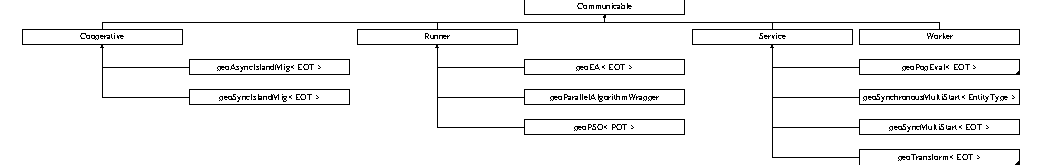
\includegraphics[height=2.22222cm]{classCommunicable}
\end{center}
\end{figure}
\subsection*{Public Member Functions}
\begin{CompactItemize}
\item 
\hypertarget{classCommunicable_8ae1827ecf7569b3db1ed386c7d8ad78}{
\hyperlink{classCommunicable_8ae1827ecf7569b3db1ed386c7d8ad78}{Communicable} ()}
\label{classCommunicable_8ae1827ecf7569b3db1ed386c7d8ad78}

\item 
\hypertarget{classCommunicable_2280b0dfa0d3a515fccf62c2a9fd5f41}{
virtual \hyperlink{classCommunicable_2280b0dfa0d3a515fccf62c2a9fd5f41}{$\sim$Communicable} ()}
\label{classCommunicable_2280b0dfa0d3a515fccf62c2a9fd5f41}

\item 
\hypertarget{classCommunicable_db4307b69b9ccacff55fdbf84b8f50e4}{
COMM\_\-ID \hyperlink{classCommunicable_db4307b69b9ccacff55fdbf84b8f50e4}{get\-Key} ()}
\label{classCommunicable_db4307b69b9ccacff55fdbf84b8f50e4}

\item 
\hypertarget{classCommunicable_e1f8bd1ee810fd73d44315c95998d19d}{
void \hyperlink{classCommunicable_e1f8bd1ee810fd73d44315c95998d19d}{lock} ()}
\label{classCommunicable_e1f8bd1ee810fd73d44315c95998d19d}

\item 
\hypertarget{classCommunicable_caa814847192e71f434fbf9479ede862}{
void \hyperlink{classCommunicable_caa814847192e71f434fbf9479ede862}{unlock} ()}
\label{classCommunicable_caa814847192e71f434fbf9479ede862}

\item 
\hypertarget{classCommunicable_cb53e6534b947bc889aa181d9dbbd13b}{
void \hyperlink{classCommunicable_cb53e6534b947bc889aa181d9dbbd13b}{stop} ()}
\label{classCommunicable_cb53e6534b947bc889aa181d9dbbd13b}

\item 
\hypertarget{classCommunicable_3306a9adb11a0ab5af342c0db9f7bb2a}{
void \hyperlink{classCommunicable_3306a9adb11a0ab5af342c0db9f7bb2a}{resume} ()}
\label{classCommunicable_3306a9adb11a0ab5af342c0db9f7bb2a}

\end{CompactItemize}
\subsection*{Protected Attributes}
\begin{CompactItemize}
\item 
\hypertarget{classCommunicable_605b0efeffe81326f216c9903f5bbf4c}{
COMM\_\-ID \hyperlink{classCommunicable_605b0efeffe81326f216c9903f5bbf4c}{key}}
\label{classCommunicable_605b0efeffe81326f216c9903f5bbf4c}

\item 
\hypertarget{classCommunicable_cf9639312f71a2f348bc1e7789ccbd9d}{
sem\_\-t \hyperlink{classCommunicable_cf9639312f71a2f348bc1e7789ccbd9d}{sem\_\-lock}}
\label{classCommunicable_cf9639312f71a2f348bc1e7789ccbd9d}

\item 
\hypertarget{classCommunicable_29c53b9191348e0505e3bcba6d8b82b1}{
sem\_\-t \hyperlink{classCommunicable_29c53b9191348e0505e3bcba6d8b82b1}{sem\_\-stop}}
\label{classCommunicable_29c53b9191348e0505e3bcba6d8b82b1}

\end{CompactItemize}
\subsection*{Static Protected Attributes}
\begin{CompactItemize}
\item 
\hypertarget{classCommunicable_7a6acfdc781a67c9c0ec4f17893f86c3}{
static unsigned \hyperlink{classCommunicable_7a6acfdc781a67c9c0ec4f17893f86c3}{num\_\-comm} = 0}
\label{classCommunicable_7a6acfdc781a67c9c0ec4f17893f86c3}

\end{CompactItemize}


\subsection{Detailed Description}




Definition at line 44 of file communicable.h.

The documentation for this class was generated from the following files:\begin{CompactItemize}
\item 
communicable.h\item 
communicable.cpp\end{CompactItemize}

\hypertarget{classCommunicator}{
\section{Communicator Class Reference}
\label{classCommunicator}\index{Communicator@{Communicator}}
}
Inheritance diagram for Communicator::\begin{figure}[H]
\begin{center}
\leavevmode
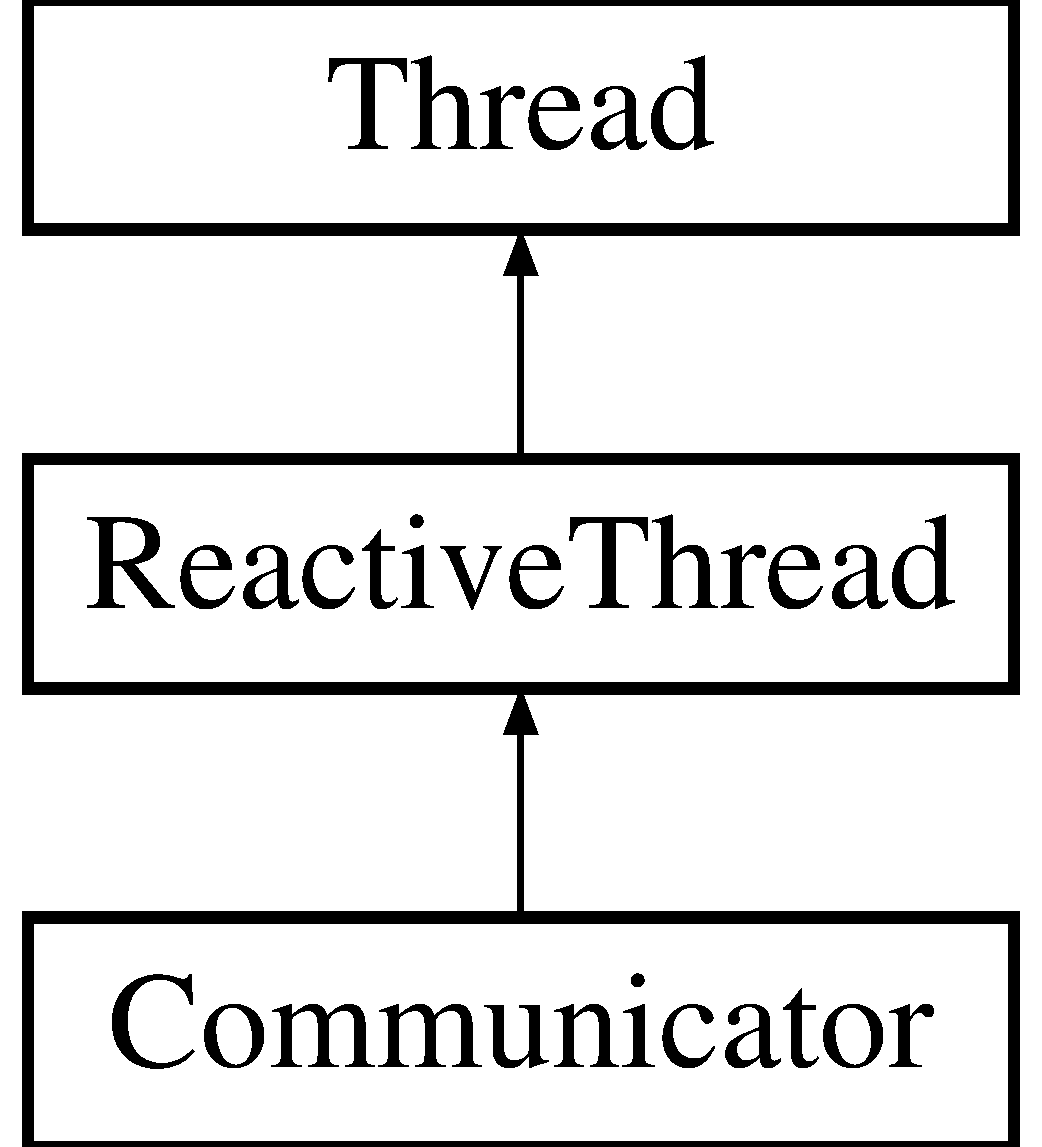
\includegraphics[height=3cm]{classCommunicator}
\end{center}
\end{figure}
\subsection*{Public Member Functions}
\begin{CompactItemize}
\item 
\hypertarget{classCommunicator_7c9dce4ea92bd04d01d53f80c0ef08ee}{
\hyperlink{classCommunicator_7c9dce4ea92bd04d01d53f80c0ef08ee}{Communicator} (int $\ast$\_\-\_\-argc, char $\ast$$\ast$$\ast$\_\-\_\-argv)}
\label{classCommunicator_7c9dce4ea92bd04d01d53f80c0ef08ee}

\item 
\hypertarget{classCommunicator_142fae13b16b166519315f248a513c62}{
void \hyperlink{classCommunicator_142fae13b16b166519315f248a513c62}{start} ()}
\label{classCommunicator_142fae13b16b166519315f248a513c62}

\end{CompactItemize}


\subsection{Detailed Description}




Definition at line 30 of file comm.h.

The documentation for this class was generated from the following files:\begin{CompactItemize}
\item 
comm.h\item 
comm.cpp\end{CompactItemize}

\hypertarget{classCooperative}{
\section{Cooperative Class Reference}
\label{classCooperative}\index{Cooperative@{Cooperative}}
}
Inheritance diagram for Cooperative::\begin{figure}[H]
\begin{center}
\leavevmode
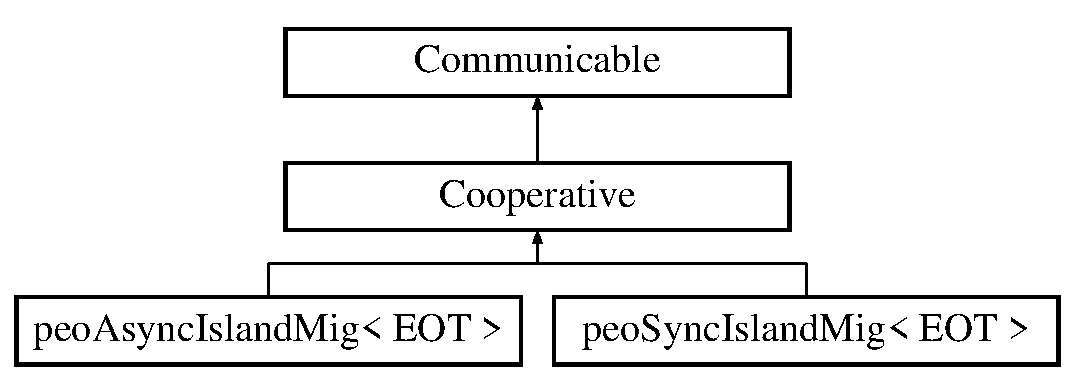
\includegraphics[height=2.53012cm]{classCooperative}
\end{center}
\end{figure}
\subsection*{Public Member Functions}
\begin{CompactItemize}
\item 
\hypertarget{classCooperative_4012b4e8329e87d26ee266491e1a883e}{
\hyperlink{classRunner}{Runner} $\ast$ \hyperlink{classCooperative_4012b4e8329e87d26ee266491e1a883e}{get\-Owner} ()}
\label{classCooperative_4012b4e8329e87d26ee266491e1a883e}

\item 
\hypertarget{classCooperative_fe7b022567174c8305bc78d8c5749b12}{
void \hyperlink{classCooperative_fe7b022567174c8305bc78d8c5749b12}{set\-Owner} (\hyperlink{classRunner}{Runner} \&\_\-\_\-runner)}
\label{classCooperative_fe7b022567174c8305bc78d8c5749b12}

\item 
\hypertarget{classCooperative_c609f2a1200da7d1ac96005602515fc6}{
void \hyperlink{classCooperative_c609f2a1200da7d1ac96005602515fc6}{send} (\hyperlink{classCooperative}{Cooperative} $\ast$\_\-\_\-coop)}
\label{classCooperative_c609f2a1200da7d1ac96005602515fc6}

\item 
\hypertarget{classCooperative_a08615f1fb5a71bb6eb8ea53ef7d1c69}{
void \hyperlink{classCooperative_a08615f1fb5a71bb6eb8ea53ef7d1c69}{synchronize\-Coop\-Ex} ()}
\label{classCooperative_a08615f1fb5a71bb6eb8ea53ef7d1c69}

\item 
\hypertarget{classCooperative_4439ddeaa1246a2e44c003bfb781739b}{
virtual void \hyperlink{classCooperative_4439ddeaa1246a2e44c003bfb781739b}{notify\-Sending} ()}
\label{classCooperative_4439ddeaa1246a2e44c003bfb781739b}

\item 
\hypertarget{classCooperative_b75a33c5735799076e01b125e47e3bbc}{
virtual void \hyperlink{classCooperative_b75a33c5735799076e01b125e47e3bbc}{notify\-Receiving} ()}
\label{classCooperative_b75a33c5735799076e01b125e47e3bbc}

\item 
\hypertarget{classCooperative_38f28f9155deac5e48edcaf935a2263b}{
virtual void \hyperlink{classCooperative_38f28f9155deac5e48edcaf935a2263b}{notify\-Sending\-Sync\-Req} ()}
\label{classCooperative_38f28f9155deac5e48edcaf935a2263b}

\item 
\hypertarget{classCooperative_6cc64e571944783b8f697f7c2299cc8d}{
virtual void \hyperlink{classCooperative_6cc64e571944783b8f697f7c2299cc8d}{notify\-Synchronized} ()}
\label{classCooperative_6cc64e571944783b8f697f7c2299cc8d}

\end{CompactItemize}
\subsection*{Private Attributes}
\begin{CompactItemize}
\item 
\hypertarget{classCooperative_7604f094479d08154ede4996a45bf79e}{
\hyperlink{classRunner}{Runner} $\ast$ \hyperlink{classCooperative_7604f094479d08154ede4996a45bf79e}{owner}}
\label{classCooperative_7604f094479d08154ede4996a45bf79e}

\end{CompactItemize}


\subsection{Detailed Description}




Definition at line 46 of file cooperative.h.

The documentation for this class was generated from the following files:\begin{CompactItemize}
\item 
cooperative.h\item 
cooperative.cpp\end{CompactItemize}

\hypertarget{classpeoAggEvalFunc}{
\section{peo\-Agg\-Eval\-Func$<$ EOT $>$ Class Template Reference}
\label{classpeoAggEvalFunc}\index{peoAggEvalFunc@{peoAggEvalFunc}}
}
The \hyperlink{classpeoAggEvalFunc}{peo\-Agg\-Eval\-Func} class offers only the interface for creating aggregate evaluation functions - there are no direct internal functions provided.  


{\tt \#include $<$peo\-Agg\-Eval\-Func.h$>$}

Inheritance diagram for peo\-Agg\-Eval\-Func$<$ EOT $>$::\begin{figure}[H]
\begin{center}
\leavevmode
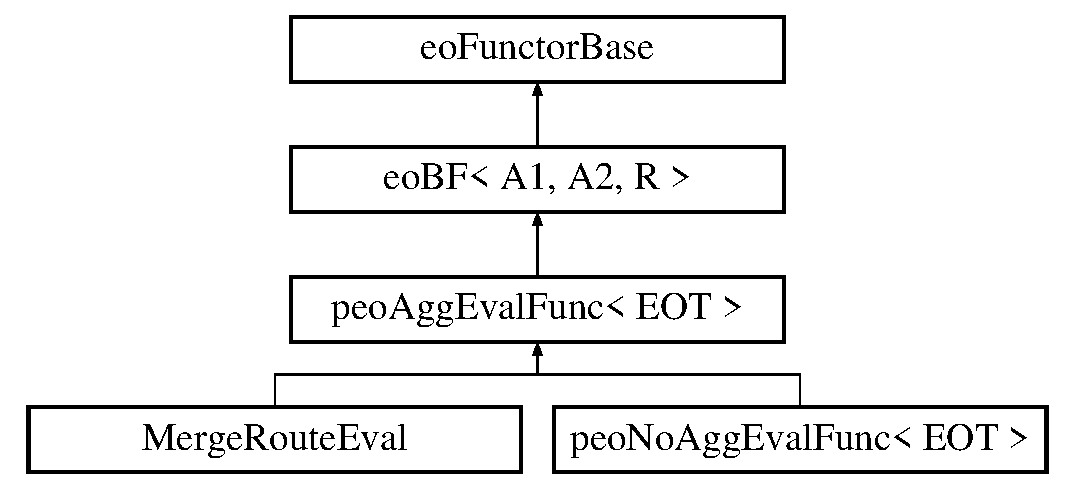
\includegraphics[height=2cm]{classpeoAggEvalFunc}
\end{center}
\end{figure}


\subsection{Detailed Description}
\subsubsection*{template$<$class EOT$>$ class peo\-Agg\-Eval\-Func$<$ EOT $>$}

The \hyperlink{classpeoAggEvalFunc}{peo\-Agg\-Eval\-Func} class offers only the interface for creating aggregate evaluation functions - there are no direct internal functions provided. 

The class inherits {\bf public eo\-BF$<$ EOT\&, const typename EOT :: Fitness\&, void $>$} thus requiring, for the derived classes, the creation of a function having the following signature:

\begin{TabularC}{2}
\hline
void operator()( EOT\& \_\-\_\-eot, const typename EOT :: Fitness\& \_\-\_\-partial\_\-fittness ); ~ &~  \\\hline
\end{TabularC}


The aggregation object is called in an iterative manner for each of the results obtained by applying partial evaluation functions. 



Definition at line 25 of file peo\-Agg\-Eval\-Func.h.

The documentation for this class was generated from the following file:\begin{CompactItemize}
\item 
peo\-Agg\-Eval\-Func.h\end{CompactItemize}

\hypertarget{classpeoAsyncIslandMig}{
\section{peo\-Async\-Island\-Mig$<$ EOT $>$ Class Template Reference}
\label{classpeoAsyncIslandMig}\index{peoAsyncIslandMig@{peoAsyncIslandMig}}
}
The \hyperlink{classpeoAsyncIslandMig}{peo\-Async\-Island\-Mig} class offers the elementary basis for implementating an asynchronous island migration model - requires the specification of several basic parameters, i.e.  


{\tt \#include $<$peo\-Async\-Island\-Mig.h$>$}

Inheritance diagram for peo\-Async\-Island\-Mig$<$ EOT $>$::\begin{figure}[H]
\begin{center}
\leavevmode
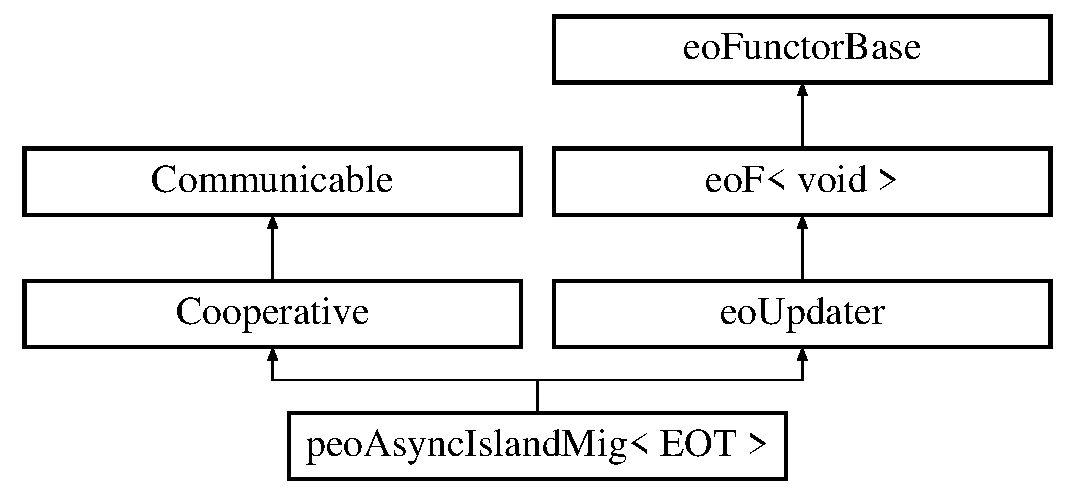
\includegraphics[height=3cm]{classpeoAsyncIslandMig}
\end{center}
\end{figure}
\subsection*{Public Member Functions}
\begin{CompactItemize}
\item 
\hyperlink{classpeoAsyncIslandMig_e0f706cbf4148d3ca327227a5c7a9fdf}{peo\-Async\-Island\-Mig} (eo\-Continue$<$ EOT $>$ \&\_\-\_\-cont, eo\-Select$<$ EOT $>$ \&\_\-\_\-select, eo\-Replacement$<$ EOT $>$ \&\_\-\_\-replace, \hyperlink{classTopology}{Topology} \&\_\-\_\-topology, eo\-Pop$<$ EOT $>$ \&\_\-\_\-source, eo\-Pop$<$ EOT $>$ \&\_\-\_\-destination)
\begin{CompactList}\small\item\em Constructor for the \hyperlink{classpeoAsyncIslandMig}{peo\-Async\-Island\-Mig} class; the characteristics of the migration model are defined through the specified parameters - out of the box objects provided in EO, etc., or custom, derived objects may be passed as parameters. \item\end{CompactList}\item 
void \hyperlink{classpeoAsyncIslandMig_13581e54425727a7f785ca8a6df527b5}{operator()} ()
\begin{CompactList}\small\item\em Function operator to be called as checkpoint for performing the migration step. \item\end{CompactList}\item 
\hypertarget{classpeoAsyncIslandMig_6d790a5d0b6ac510cac4f61a1c0d8f16}{
void \hyperlink{classpeoAsyncIslandMig_6d790a5d0b6ac510cac4f61a1c0d8f16}{pack} ()}
\label{classpeoAsyncIslandMig_6d790a5d0b6ac510cac4f61a1c0d8f16}

\begin{CompactList}\small\item\em Auxiliary function dealing with sending the emigrant individuals. There is no need to explicitly call the function. \item\end{CompactList}\item 
\hypertarget{classpeoAsyncIslandMig_455501aee5db2bbfbae15779c8429369}{
void \hyperlink{classpeoAsyncIslandMig_455501aee5db2bbfbae15779c8429369}{unpack} ()}
\label{classpeoAsyncIslandMig_455501aee5db2bbfbae15779c8429369}

\begin{CompactList}\small\item\em Auxiliary function dealing with receiving immigrant individuals. There is no need to explicitly call the function. \item\end{CompactList}\end{CompactItemize}
\subsection*{Private Member Functions}
\begin{CompactItemize}
\item 
\hypertarget{classpeoAsyncIslandMig_87a4ef7d4bd30d349a801bf0f9e87c82}{
void \hyperlink{classpeoAsyncIslandMig_87a4ef7d4bd30d349a801bf0f9e87c82}{emigrate} ()}
\label{classpeoAsyncIslandMig_87a4ef7d4bd30d349a801bf0f9e87c82}

\item 
\hypertarget{classpeoAsyncIslandMig_5a9a64ba51a696e45f91b362c39c9a64}{
void \hyperlink{classpeoAsyncIslandMig_5a9a64ba51a696e45f91b362c39c9a64}{immigrate} ()}
\label{classpeoAsyncIslandMig_5a9a64ba51a696e45f91b362c39c9a64}

\end{CompactItemize}
\subsection*{Private Attributes}
\begin{CompactItemize}
\item 
\hypertarget{classpeoAsyncIslandMig_2fc077d02ef9ea4595cfe883af0d4f83}{
eo\-Continue$<$ EOT $>$ \& \hyperlink{classpeoAsyncIslandMig_2fc077d02ef9ea4595cfe883af0d4f83}{cont}}
\label{classpeoAsyncIslandMig_2fc077d02ef9ea4595cfe883af0d4f83}

\item 
\hypertarget{classpeoAsyncIslandMig_b1fa045094c8a411323e75b5820c80c2}{
eo\-Select$<$ EOT $>$ \& \hyperlink{classpeoAsyncIslandMig_b1fa045094c8a411323e75b5820c80c2}{select}}
\label{classpeoAsyncIslandMig_b1fa045094c8a411323e75b5820c80c2}

\item 
\hypertarget{classpeoAsyncIslandMig_b761dbd880ee32e170741ecd78da6f48}{
eo\-Replacement$<$ EOT $>$ \& \hyperlink{classpeoAsyncIslandMig_b761dbd880ee32e170741ecd78da6f48}{replace}}
\label{classpeoAsyncIslandMig_b761dbd880ee32e170741ecd78da6f48}

\item 
\hypertarget{classpeoAsyncIslandMig_e45e5a808a96f0853ab6ba42339fe679}{
\hyperlink{classTopology}{Topology} \& \hyperlink{classpeoAsyncIslandMig_e45e5a808a96f0853ab6ba42339fe679}{topology}}
\label{classpeoAsyncIslandMig_e45e5a808a96f0853ab6ba42339fe679}

\item 
\hypertarget{classpeoAsyncIslandMig_8a502d82c773033e274dca932fc2d4ee}{
eo\-Pop$<$ EOT $>$ \& \hyperlink{classpeoAsyncIslandMig_8a502d82c773033e274dca932fc2d4ee}{source}}
\label{classpeoAsyncIslandMig_8a502d82c773033e274dca932fc2d4ee}

\item 
\hypertarget{classpeoAsyncIslandMig_e407f411d08ae7d96992603c145a7e43}{
eo\-Pop$<$ EOT $>$ \& \hyperlink{classpeoAsyncIslandMig_e407f411d08ae7d96992603c145a7e43}{destination}}
\label{classpeoAsyncIslandMig_e407f411d08ae7d96992603c145a7e43}

\item 
\hypertarget{classpeoAsyncIslandMig_b8c76d98d9ae99dd930a77c12860519a}{
std::queue$<$ eo\-Pop$<$ EOT $>$ $>$ \hyperlink{classpeoAsyncIslandMig_b8c76d98d9ae99dd930a77c12860519a}{imm}}
\label{classpeoAsyncIslandMig_b8c76d98d9ae99dd930a77c12860519a}

\item 
\hypertarget{classpeoAsyncIslandMig_a9cc0e2d61cac6e11647b141962adc89}{
std::queue$<$ eo\-Pop$<$ EOT $>$ $>$ \hyperlink{classpeoAsyncIslandMig_a9cc0e2d61cac6e11647b141962adc89}{em}}
\label{classpeoAsyncIslandMig_a9cc0e2d61cac6e11647b141962adc89}

\item 
\hypertarget{classpeoAsyncIslandMig_1a2c0004d23bc303420af137a8c8bd27}{
std::queue$<$ \hyperlink{classCooperative}{Cooperative} $\ast$ $>$ \hyperlink{classpeoAsyncIslandMig_1a2c0004d23bc303420af137a8c8bd27}{coop\_\-em}}
\label{classpeoAsyncIslandMig_1a2c0004d23bc303420af137a8c8bd27}

\end{CompactItemize}


\subsection{Detailed Description}
\subsubsection*{template$<$class EOT$>$ class peo\-Async\-Island\-Mig$<$ EOT $>$}

The \hyperlink{classpeoAsyncIslandMig}{peo\-Async\-Island\-Mig} class offers the elementary basis for implementating an asynchronous island migration model - requires the specification of several basic parameters, i.e. 

continuation criterion, selection and replacement strategies, a topological model and the source and destination population for the migrating individuals. As opposed to the synchronous migration model, in the asynchronous migration approach, there is no synchronization step between islands after performing the emigration phase.

The migration operator is called at the end of each generation of an evolutionary algorithms as a checkpoint object - the following code exposes the structure of a classic evolutionary algorithm:

\begin{TabularC}{2}
\hline
{\bf do} \{ ~ &~  \\\hline
~~~~~~~~ select( population, offsprings ); ~ &// select the offsprings from the current population \\\hline
~~~~~~~~ transform( offsprings ); ~ &// crossover and mutation operators are applied on the selected offsprings \\\hline
~~~~~~~~ evaluate( offsprings ); ~ &// evaluation step of the resulting offsprings \\\hline
~~~~~~~~ replace( population, offsprings ); ~ &// replace the individuals in the current population whith individuals from the offspring population, according to a specified replacement strategy \\\hline
\} {\bf while} ( ea\-Checkpoint\-Continue( population ) ); ~ &// checkpoint operators are applied on the current population, including the migration operator, if any specified  \\\hline
\end{TabularC}


Constructing an asynchronous island migration model requires having defined (1) a topological migration model, (2) the control parameters of the migration process, (3) a checkpoint object associated with an evolutionary algorithm, and (4) an owner object must be set. The owner object must be derived from the {\bf \hyperlink{classRunner}{Runner}} class (for example a \hyperlink{classpeoEA}{peo\-EA} object represents a possible owner). A simple example is offered bellow:

\begin{enumerate}
\item topological model to be followed when performing migrations: \par
 \par
 \begin{TabularC}{2}
\hline
\hyperlink{classRingTopology}{Ring\-Topology} mig\-Topology; ~ &// a simple ring topological model - each island communicates with two other islands \\\hline
\end{TabularC}


\item the continuation criterion, selection and replacement strategy etc. are defined: \par
 \par
 \begin{TabularC}{2}
\hline
eo\-Pop$<$ EOT $>$ population( POP\_\-SIZE, pop\-Initializer ); ~ &// population of individuals to be used for the evolutionary algorithm \\\hline
~  &~  \\\hline
eo\-Periodic\-Continue$<$ EOT $>$ mig\-Cont( MIG\_\-FREQ ); ~ &// migrations occur periodically at MIG\_\-FREQ iterations \\\hline
eo\-Random\-Select$<$ EOT $>$ mig\-Select\-Strategy; ~ &// selection strategy - in this case a random selection is applied \\\hline
eo\-Select\-Number$<$ EOT $>$ mig\-Select( mig\-Select\-Strategy, MIG\_\-SIZE ); ~ &// number of individuals to be selected using the specified strategy \\\hline
eo\-Plus\-Replacement$<$ EOT $>$ mig\-Replace; ~ &// immigration strategy - the worse individuals in the destination population are replaced by the immigrant individuals \\\hline
~  &~  \\\hline
peo\-Async\-Island\-Mig$<$ EOT $>$ async\-Migration( \par
 ~~~~~~~~ mig\-Cont, mig\-Select, mig\-Replace, mig\-Topology, \par
 ~~~~~~~~ population, population \par
 ); ~  &// asynchronous migration object - the emigrant individuals are selected from the same from population in which the immigrant individuals are being integrated  \\\hline
\end{TabularC}


\item creation of a checkpoint object as part of the definition of an evolutionary algoritm (details of th EA not given as being out of scope): \par
 \par
 \begin{TabularC}{2}
\hline
... ~ &~  \\\hline
eo\-Gen\-Continue$<$ EOT $>$ ea\-Cont( NUM\_\-GEN ); ~ &// the evolutionary algorithm will stop after NUM\_\-GEN generations \\\hline
eo\-Check\-Point$<$ EOT $>$ ea\-Checkpoint\-Continue( ea\-Cont ); ~ &// number of individuals to be selected using the specified strategy \\\hline
... ~ &~  \\\hline
ea\-Checkpoint\-Continue.add( async\-Migration ); ~ &// adding the migration operator as checkpoint element \\\hline
... ~ &~  \\\hline
\end{TabularC}


\item definition of an owner evolutionary algorithm (an object inheriting the {\bf \hyperlink{classRunner}{Runner}} class): \par
 \par
 \begin{TabularC}{2}
\hline
peo\-EA$<$ EOT $>$ ea\-Alg( ea\-Checkpoint\-Continue, ea\-Pop\-Eval, ea\-Select, ea\-Transform, ea\-Replace); ~ &// evolutionary algorithm having as checkpoint the ea\-Checkpoint\-Continue object defined above  \\\hline
async\-Migration.set\-Owner( ea\-Alg ); ~ &// setting the evolutionary algorithm as owner of the migration object  \\\hline
ea\-Alg( population ); ~ &// applying the evolutionary algorithm on a given population  \\\hline
\end{TabularC}
\end{enumerate}


The source and the destination population for the migration object were specified as being the same, in step no. 2, as we are usually interested in selecting the emigrants and integrating the immigrant individuals from and in, respectively, one unique population, iteratively evolved by an evolutionary algorithm. There is no restriction in having two distinct populations as source and destination for the emigrant and immigrant individuals respectively.

The above steps only create an asynchronous migration object associated to an evolutionary algorithm. The creation of several islands requires the reiteration of the steps 2 through 4 for creating distinct algorithms, with distinct populations and the associated distinctly parametrized migration objects. The interconnecting element is the underlying topology, defined at step 1 (the same C++ mig\-Topology object has to be passed as parameter for all the migration objects, in order to interconnect them). 



Definition at line 112 of file peo\-Async\-Island\-Mig.h.

\subsection{Constructor \& Destructor Documentation}
\hypertarget{classpeoAsyncIslandMig_e0f706cbf4148d3ca327227a5c7a9fdf}{
\index{peoAsyncIslandMig@{peo\-Async\-Island\-Mig}!peoAsyncIslandMig@{peoAsyncIslandMig}}
\index{peoAsyncIslandMig@{peoAsyncIslandMig}!peoAsyncIslandMig@{peo\-Async\-Island\-Mig}}
\subsubsection[peoAsyncIslandMig]{\setlength{\rightskip}{0pt plus 5cm}template$<$class EOT$>$ \hyperlink{classpeoAsyncIslandMig}{peo\-Async\-Island\-Mig}$<$ EOT $>$::\hyperlink{classpeoAsyncIslandMig}{peo\-Async\-Island\-Mig} (eo\-Continue$<$ EOT $>$ \& {\em \_\-\_\-cont}, eo\-Select$<$ EOT $>$ \& {\em \_\-\_\-select}, eo\-Replacement$<$ EOT $>$ \& {\em \_\-\_\-replace}, \hyperlink{classTopology}{Topology} \& {\em \_\-\_\-topology}, eo\-Pop$<$ EOT $>$ \& {\em \_\-\_\-source}, eo\-Pop$<$ EOT $>$ \& {\em \_\-\_\-destination})}}
\label{classpeoAsyncIslandMig_e0f706cbf4148d3ca327227a5c7a9fdf}


Constructor for the \hyperlink{classpeoAsyncIslandMig}{peo\-Async\-Island\-Mig} class; the characteristics of the migration model are defined through the specified parameters - out of the box objects provided in EO, etc., or custom, derived objects may be passed as parameters. 

\begin{Desc}
\item[Parameters:]
\begin{description}
\item[{\em eo\-Continue$<$}]EOT $>$\& \_\-\_\-cont - continuation criterion specifying whether the migration is performed or not; \item[{\em eo\-Select$<$}]EOT $>$\& \_\-\_\-select - selection strategy to be applied for constructing a list of emigrant individuals out of the source population; \item[{\em eo\-Replacement$<$}]EOT $>$\& \_\-\_\-replace - replacement strategy used for integrating the immigrant individuals in the destination population; \item[{\em Topology\&}]\_\-\_\-topology - topological model to be followed when performing migrations; \item[{\em eo\-Pop$<$}]EOT $>$\& \_\-\_\-source - source population from which the emigrant individuals are selected; \item[{\em eo\-Pop$<$}]EOT $>$\& \_\-\_\-destination - destination population in which the immigrant population are integrated. \end{description}
\end{Desc}


Definition at line 171 of file peo\-Async\-Island\-Mig.h.

References Topology::add().

\subsection{Member Function Documentation}
\hypertarget{classpeoAsyncIslandMig_13581e54425727a7f785ca8a6df527b5}{
\index{peoAsyncIslandMig@{peo\-Async\-Island\-Mig}!operator()@{operator()}}
\index{operator()@{operator()}!peoAsyncIslandMig@{peo\-Async\-Island\-Mig}}
\subsubsection[operator()]{\setlength{\rightskip}{0pt plus 5cm}template$<$class EOT$>$ void \hyperlink{classpeoAsyncIslandMig}{peo\-Async\-Island\-Mig}$<$ EOT $>$::operator() ()}}
\label{classpeoAsyncIslandMig_13581e54425727a7f785ca8a6df527b5}


Function operator to be called as checkpoint for performing the migration step. 

The emigrant individuals are selected from the source population and sent to the next island (defined by the topology object) while the immigrant individuals are integrated in the destination population. There is no need to explicitly call the function - the wrapper checkpoint object (please refer to the above example) will perform the call when required. 

Definition at line 248 of file peo\-Async\-Island\-Mig.h.

References peo\-Async\-Island\-Mig$<$ EOT $>$::cont, peo\-Async\-Island\-Mig$<$ EOT $>$::emigrate(), peo\-Async\-Island\-Mig$<$ EOT $>$::immigrate(), and peo\-Async\-Island\-Mig$<$ EOT $>$::source.

The documentation for this class was generated from the following file:\begin{CompactItemize}
\item 
peo\-Async\-Island\-Mig.h\end{CompactItemize}

\hypertarget{classpeoEA}{
\section{peo\-EA$<$ EOT $>$ Class Template Reference}
\label{classpeoEA}\index{peoEA@{peoEA}}
}
The \hyperlink{classpeoEA}{peo\-EA} class offers an elementary evolutionary algorithm implementation.  


{\tt \#include $<$peo\-EA.h$>$}

Inheritance diagram for peo\-EA$<$ EOT $>$::\begin{figure}[H]
\begin{center}
\leavevmode
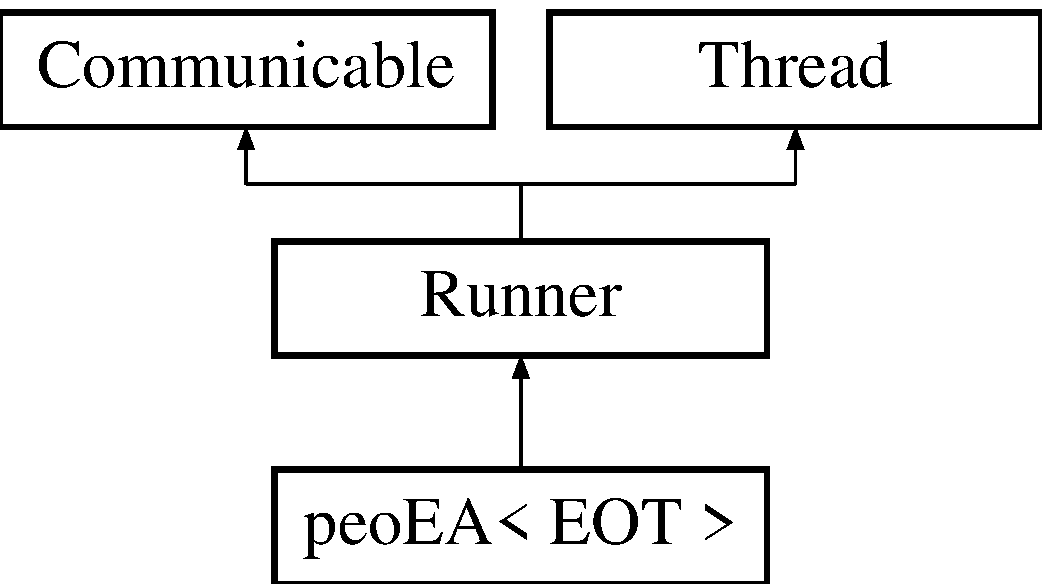
\includegraphics[height=3cm]{classpeoEA}
\end{center}
\end{figure}
\subsection*{Public Member Functions}
\begin{CompactItemize}
\item 
\hyperlink{classpeoEA_dbfc4f8907bef234602149229f132371}{peo\-EA} (\bf{eo\-Continue}$<$ EOT $>$ \&\_\-\_\-cont, \hyperlink{classpeoPopEval}{peo\-Pop\-Eval}$<$ EOT $>$ \&\_\-\_\-pop\_\-eval, \bf{eo\-Select}$<$ EOT $>$ \&\_\-\_\-select, \hyperlink{classpeoTransform}{peo\-Transform}$<$ EOT $>$ \&\_\-\_\-trans, \bf{eo\-Replacement}$<$ EOT $>$ \&\_\-\_\-replace)
\begin{CompactList}\small\item\em Constructor for the evolutionary algorithm object - several basic parameters have to be specified, allowing for different levels of parallelism. \item\end{CompactList}\item 
\hypertarget{classpeoEA_6ab8c321d29350634143a2a01cf2ad24}{
void \hyperlink{classpeoEA_6ab8c321d29350634143a2a01cf2ad24}{run} ()}
\label{classpeoEA_6ab8c321d29350634143a2a01cf2ad24}

\begin{CompactList}\small\item\em Evolutionary algorithm function - a side effect of the fact that the class is derived from the {\bf \hyperlink{classRunner}{Runner}} class, thus requiring the existence of a {\em run\/} function, the algorithm being executed on a distinct thread. \item\end{CompactList}\item 
void \hyperlink{classpeoEA_3c709e3b2491147d26fee36138644613}{operator()} (\bf{eo\-Pop}$<$ EOT $>$ \&\_\-\_\-pop)
\begin{CompactList}\small\item\em \doxyref{Function} operator for specifying the population to be associated with the algorithm. \item\end{CompactList}\end{CompactItemize}
\subsection*{Private Attributes}
\begin{CompactItemize}
\item 
\hypertarget{classpeoEA_5f015eebf42f176b9fe322488c446c2a}{
\bf{eo\-Continue}$<$ EOT $>$ \& \hyperlink{classpeoEA_5f015eebf42f176b9fe322488c446c2a}{cont}}
\label{classpeoEA_5f015eebf42f176b9fe322488c446c2a}

\item 
\hypertarget{classpeoEA_9140259f50c9186edcb062b023624c96}{
\hyperlink{classpeoPopEval}{peo\-Pop\-Eval}$<$ EOT $>$ \& \hyperlink{classpeoEA_9140259f50c9186edcb062b023624c96}{pop\_\-eval}}
\label{classpeoEA_9140259f50c9186edcb062b023624c96}

\item 
\hypertarget{classpeoEA_2d8428d69fdd6aefefbaf543fdd46d19}{
\bf{eo\-Select}$<$ EOT $>$ \& \hyperlink{classpeoEA_2d8428d69fdd6aefefbaf543fdd46d19}{select}}
\label{classpeoEA_2d8428d69fdd6aefefbaf543fdd46d19}

\item 
\hypertarget{classpeoEA_713c77935eb8aafebfb9488cfaa4a363}{
\hyperlink{classpeoTransform}{peo\-Transform}$<$ EOT $>$ \& \hyperlink{classpeoEA_713c77935eb8aafebfb9488cfaa4a363}{trans}}
\label{classpeoEA_713c77935eb8aafebfb9488cfaa4a363}

\item 
\hypertarget{classpeoEA_9bd2d4356cf7e69e3141dc269213aa8a}{
\bf{eo\-Replacement}$<$ EOT $>$ \& \hyperlink{classpeoEA_9bd2d4356cf7e69e3141dc269213aa8a}{replace}}
\label{classpeoEA_9bd2d4356cf7e69e3141dc269213aa8a}

\item 
\hypertarget{classpeoEA_c0b110e410bc16283e8339f24b733772}{
\bf{eo\-Pop}$<$ EOT $>$ $\ast$ \hyperlink{classpeoEA_c0b110e410bc16283e8339f24b733772}{pop}}
\label{classpeoEA_c0b110e410bc16283e8339f24b733772}

\end{CompactItemize}


\subsection{Detailed Description}
\subsubsection*{template$<$class EOT$>$ class peo\-EA$<$ EOT $>$}

The \hyperlink{classpeoEA}{peo\-EA} class offers an elementary evolutionary algorithm implementation. 

In addition, as compared with the algorithms provided by the \doxyref{EO} framework, the \hyperlink{classpeoEA}{peo\-EA} class has the underlying necessary structure for including, for example, parallel evaluation and parallel transformation operators, migration operators etc. Although there is no restriction on using the algorithms provided by the \doxyref{EO} framework, the drawback resides in the fact that the \doxyref{EO} implementation is exclusively sequential and, in consequence, no parallelism is provided. A simple example for constructing a \hyperlink{classpeoEA}{peo\-EA} object:

\begin{TabularC}{2}
\hline
... ~ &~  \\\hline
eo\-Pop$<$ EOT $>$ population( POP\_\-SIZE, pop\-Initializer ); ~ &// creation of a population with POP\_\-SIZE individuals - the pop\-Initializer is a functor to be called for each individual \\\hline
~  &~  \\\hline
eo\-Gen\-Continue$<$ EOT $>$ ea\-Cont( NUM\_\-GEN ); ~ &// number of generations for the evolutionary algorithm \\\hline
eo\-Check\-Point$<$ EOT $>$ ea\-Checkpoint\-Continue( ea\-Cont ); ~ &// checkpoint incorporating the continuation criterion - startpoint for adding other checkpoint objects \\\hline
~  &~  \\\hline
peo\-Seq\-Pop\-Eval$<$ EOT $>$ ea\-Pop\-Eval( eval\-Function ); ~ &// sequential evaluation functor wrapper - eval\-Function represents the actual evaluation functor  \\\hline
~  &~  \\\hline
eo\-Ranking\-Select$<$ EOT $>$ selection\-Strategy; ~ &// selection strategy for creating the offspring population - a simple ranking selection in this case  \\\hline
eo\-Select\-Number$<$ EOT $>$ ea\-Select( selection\-Strategy, POP\_\-SIZE ); ~ &// the number of individuals to be selected for creating the offspring population  \\\hline
eo\-Ranking\-Select$<$ EOT $>$ selection\-Strategy; ~ &// selection strategy for creating the offspring population - a simple ranking selection in this case  \\\hline
~  &~  \\\hline
eo\-SGATransform$<$ EOT $>$ transform( crossover, CROSS\_\-RATE, mutation, MUT\_\-RATE ); ~ &// transformation operator - crossover and mutation operators with their associated probabilities  \\\hline
peo\-Seq\-Transform$<$ EOT $>$ ea\-Transform( transform ); ~ &// Paradis\-EO specific sequential operator - a parallel version may be specified in the same manner  \\\hline
~  &~  \\\hline
eo\-Plus\-Replacement$<$ EOT $>$ ea\-Replace; ~ &// replacement strategy - for integrating the offspring resulting individuals in the initial population  \\\hline
~  &~  \\\hline
peo\-EA$<$ EOT $>$ ea\-Alg( ea\-Checkpoint\-Continue, ea\-Pop\-Eval, ea\-Select, ea\-Transform, ea\-Replace ); ~ &// Paradis\-EO evolutionary algorithm integrating the above defined objects  \\\hline
ea\-Alg( population ); ~ &// specifying the initial population for the algorithm  \\\hline
... ~ &~  \\\hline
\end{TabularC}




Definition at line 54 of file peo\-EA.h.

\subsection{Constructor \& Destructor Documentation}
\hypertarget{classpeoEA_dbfc4f8907bef234602149229f132371}{
\index{peoEA@{peo\-EA}!peoEA@{peoEA}}
\index{peoEA@{peoEA}!peoEA@{peo\-EA}}
\subsubsection[peoEA]{\setlength{\rightskip}{0pt plus 5cm}template$<$class EOT$>$ \hyperlink{classpeoEA}{peo\-EA}$<$ EOT $>$::\hyperlink{classpeoEA}{peo\-EA} (\bf{eo\-Continue}$<$ EOT $>$ \& {\em \_\-\_\-cont}, \hyperlink{classpeoPopEval}{peo\-Pop\-Eval}$<$ EOT $>$ \& {\em \_\-\_\-pop\_\-eval}, \bf{eo\-Select}$<$ EOT $>$ \& {\em \_\-\_\-select}, \hyperlink{classpeoTransform}{peo\-Transform}$<$ EOT $>$ \& {\em \_\-\_\-trans}, \bf{eo\-Replacement}$<$ EOT $>$ \& {\em \_\-\_\-replace})}}
\label{classpeoEA_dbfc4f8907bef234602149229f132371}


Constructor for the evolutionary algorithm object - several basic parameters have to be specified, allowing for different levels of parallelism. 

Depending on the requirements, a sequential or a parallel evaluation operator may be specified or, in the same manner, a sequential or a parallel transformation operator may be given as parameter. Out of the box objects may be provided, from the \doxyref{EO} package, for example, or custom defined ones may be specified, provided that they are derived from the correct base classes.

\begin{Desc}
\item[Parameters:]
\begin{description}
\item[{\em eo\-Continue$<$}]EOT $>$\& \_\-\_\-cont - continuation criterion specifying whether the algorithm should continue or not; \item[{\em peo\-Pop\-Eval$<$}]EOT $>$\& \_\-\_\-pop\_\-eval - evaluation operator; it allows the specification of parallel evaluation operators, aggregate evaluation functions, etc.; \item[{\em eo\-Select$<$}]EOT $>$\& \_\-\_\-select - selection strategy to be applied for constructing a list of offspring individuals; \item[{\em peo\-Transform$<$}]EOT $>$\& \_\-\_\-trans - transformation operator, i.e. crossover and mutation; allows for sequential or parallel transform; \item[{\em eo\-Replacement$<$}]EOT $>$\& \_\-\_\-replace - replacement strategy for integrating the offspring individuals in the initial population; \end{description}
\end{Desc}


Definition at line 98 of file peo\-EA.h.

References peo\-EA$<$ EOT $>$::pop\_\-eval, and peo\-EA$<$ EOT $>$::trans.

\subsection{Member Function Documentation}
\hypertarget{classpeoEA_3c709e3b2491147d26fee36138644613}{
\index{peoEA@{peo\-EA}!operator()@{operator()}}
\index{operator()@{operator()}!peoEA@{peo\-EA}}
\subsubsection[operator()]{\setlength{\rightskip}{0pt plus 5cm}template$<$class EOT$>$ void \hyperlink{classpeoEA}{peo\-EA}$<$ EOT $>$::operator() (\bf{eo\-Pop}$<$ EOT $>$ \& {\em \_\-\_\-pop})}}
\label{classpeoEA_3c709e3b2491147d26fee36138644613}


\doxyref{Function} operator for specifying the population to be associated with the algorithm. 

\begin{Desc}
\item[Parameters:]
\begin{description}
\item[{\em eo\-Pop$<$}]EOT $>$\& \_\-\_\-pop - initial population of the algorithm, to be iteratively evolved; \end{description}
\end{Desc}


Definition at line 114 of file peo\-EA.h.

References peo\-EA$<$ EOT $>$::pop.

The documentation for this class was generated from the following file:\begin{CompactItemize}
\item 
peo\-EA.h\end{CompactItemize}

\hypertarget{classpeoNoAggEvalFunc}{
\section{peo\-No\-Agg\-Eval\-Func$<$ EOT $>$ Class Template Reference}
\label{classpeoNoAggEvalFunc}\index{peoNoAggEvalFunc@{peoNoAggEvalFunc}}
}
The \hyperlink{classpeoNoAggEvalFunc}{peo\-No\-Agg\-Eval\-Func} class does nothing more than an association between a fitness value and a specified individual.  


{\tt \#include $<$peo\-No\-Agg\-Eval\-Func.h$>$}

Inheritance diagram for peo\-No\-Agg\-Eval\-Func$<$ EOT $>$::\begin{figure}[H]
\begin{center}
\leavevmode
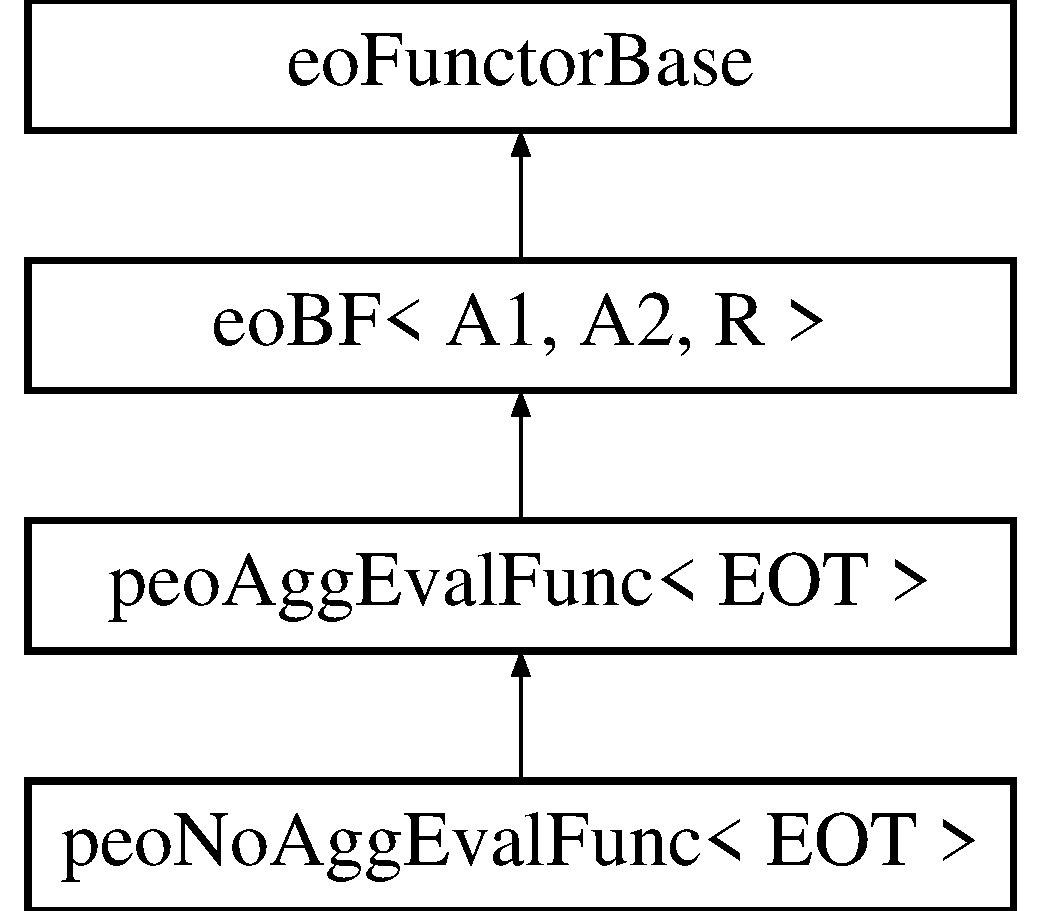
\includegraphics[height=4cm]{classpeoNoAggEvalFunc}
\end{center}
\end{figure}
\subsection*{Public Member Functions}
\begin{CompactItemize}
\item 
\hypertarget{classpeoNoAggEvalFunc_1a69ee1af8745ac75c864bf884436de5}{
void \hyperlink{classpeoNoAggEvalFunc_1a69ee1af8745ac75c864bf884436de5}{operator()} (EOT \&\_\-\_\-sol, const typename EOT::Fitness \&\_\-\_\-fit)}
\label{classpeoNoAggEvalFunc_1a69ee1af8745ac75c864bf884436de5}

\begin{CompactList}\small\item\em Operator which sets as fitness the {\bf \_\-\_\-fit} value for the {\bf \_\-\_\-sol} individual. \item\end{CompactList}\end{CompactItemize}


\subsection{Detailed Description}
\subsubsection*{template$<$class EOT$>$ class peo\-No\-Agg\-Eval\-Func$<$ EOT $>$}

The \hyperlink{classpeoNoAggEvalFunc}{peo\-No\-Agg\-Eval\-Func} class does nothing more than an association between a fitness value and a specified individual. 

The class is provided as a mean of declaring that no aggregation is required for the evaluation function - the fitness value is explicitly specified. 



Definition at line 47 of file peo\-No\-Agg\-Eval\-Func.h.

The documentation for this class was generated from the following file:\begin{CompactItemize}
\item 
peo\-No\-Agg\-Eval\-Func.h\end{CompactItemize}

\hypertarget{classpeoParaPopEval}{
\section{peo\-Para\-Pop\-Eval$<$ EOT $>$ Class Template Reference}
\label{classpeoParaPopEval}\index{peoParaPopEval@{peoParaPopEval}}
}
The \hyperlink{classpeoParaPopEval}{peo\-Para\-Pop\-Eval} represents a wrapper for creating a functor capable of applying in parallel an EO-derived evaluation functor.  


{\tt \#include $<$peo\-Para\-Pop\-Eval.h$>$}

Inheritance diagram for peo\-Para\-Pop\-Eval$<$ EOT $>$::\begin{figure}[H]
\begin{center}
\leavevmode
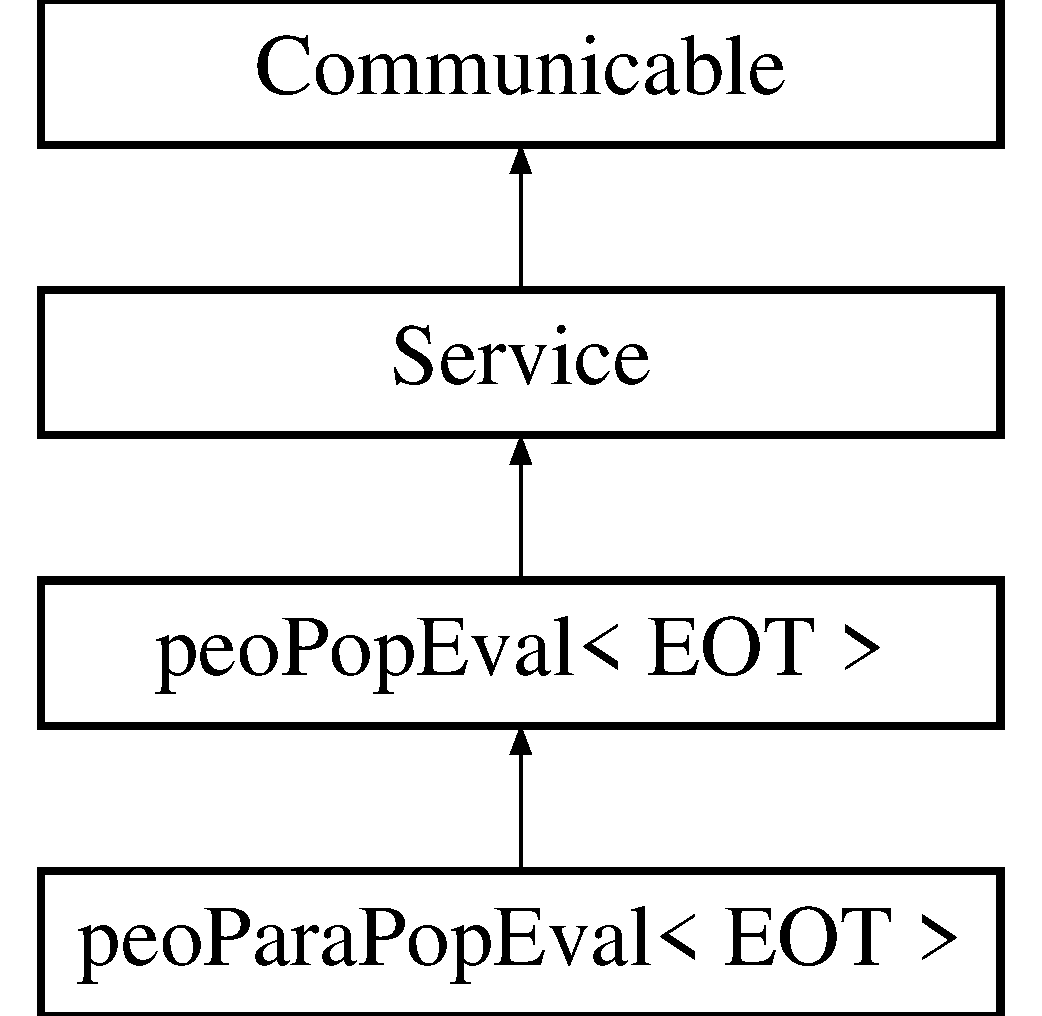
\includegraphics[height=4cm]{classpeoParaPopEval}
\end{center}
\end{figure}
\subsection*{Public Member Functions}
\begin{CompactItemize}
\item 
\hyperlink{classpeoParaPopEval_bcb540510a7038520bec41a7af332daf}{peo\-Para\-Pop\-Eval} (eo\-Eval\-Func$<$ EOT $>$ \&\_\-\_\-eval\_\-func)
\begin{CompactList}\small\item\em Constructor function - an EO-derived evaluation functor has to be specified; an internal reference is set towards the specified evaluation functor. \item\end{CompactList}\item 
\hyperlink{classpeoParaPopEval_1cc13a1ec366f95d219d682eccb455bc}{peo\-Para\-Pop\-Eval} (const std::vector$<$ eo\-Eval\-Func$<$ EOT $>$ $\ast$ $>$ \&\_\-\_\-funcs, \hyperlink{classpeoAggEvalFunc}{peo\-Agg\-Eval\-Func}$<$ EOT $>$ \&\_\-\_\-merge\_\-eval)
\begin{CompactList}\small\item\em Constructor function - a vector of EO-derived evaluation functors has to be specified as well as an aggregation function. \item\end{CompactList}\item 
void \hyperlink{classpeoParaPopEval_aeaa4fca4f8650e453e308838b4a2cb5}{operator()} (eo\-Pop$<$ EOT $>$ \&\_\-\_\-pop)
\begin{CompactList}\small\item\em Operator for applying the evaluation functor (direct or aggregate) for each individual of the specified population. \item\end{CompactList}\item 
void \hyperlink{classpeoParaPopEval_fea632bd645ab11182782fd3c038d6d8}{pack\-Data} ()
\begin{CompactList}\small\item\em Auxiliary function for transferring data between the process requesting an evaluation operation and the process that performs the actual evaluation phase. \item\end{CompactList}\item 
void \hyperlink{classpeoParaPopEval_410bf4c173e2f36df82251cb16ce1b05}{unpack\-Data} ()
\begin{CompactList}\small\item\em Auxiliary function for transferring data between the process requesting an evaluation operation and the process that performs the actual evaluation phase. \item\end{CompactList}\item 
\hypertarget{classpeoParaPopEval_3af76378611eac5a36da9a0a00aeeb6c}{
void \hyperlink{classpeoParaPopEval_3af76378611eac5a36da9a0a00aeeb6c}{execute} ()}
\label{classpeoParaPopEval_3af76378611eac5a36da9a0a00aeeb6c}

\begin{CompactList}\small\item\em Auxiliary function - it calls the specified evaluation functor(s). There is no need to explicitly call the function. \item\end{CompactList}\item 
void \hyperlink{classpeoParaPopEval_24bb4ae84b0b9f64e7170e3d2b0e1223}{pack\-Result} ()
\begin{CompactList}\small\item\em Auxiliary function for transferring data between the process requesting an evaluation operation and the process that performs the actual evaluation phase. \item\end{CompactList}\item 
void \hyperlink{classpeoParaPopEval_fd7f0afe9cba30be39269d16097e190e}{unpack\-Result} ()
\begin{CompactList}\small\item\em Auxiliary function for transferring data between the process requesting an evaluation operation and the process that performs the actual evaluation phase. \item\end{CompactList}\item 
void \hyperlink{classpeoParaPopEval_1f78c3cec2940af08a059cc1aa96a9c8}{notify\-Sending\-Data} ()
\begin{CompactList}\small\item\em Auxiliary function for notifications between the process requesting an evaluation operation and the processes that performs the actual evaluation phase. \item\end{CompactList}\item 
void \hyperlink{classpeoParaPopEval_b77031fc4807921ffaf7cf6b669a7665}{notify\-Sending\-All\-Resource\-Requests} ()
\begin{CompactList}\small\item\em Auxiliary function for notifications between the process requesting an evaluation operation and the processes that performs the actual evaluation phase. \item\end{CompactList}\end{CompactItemize}
\subsection*{Private Attributes}
\begin{CompactItemize}
\item 
\hypertarget{classpeoParaPopEval_6d69b8f73c0b5d72baf75d6e53f025b7}{
const std::vector$<$ eo\-Eval\-Func$<$ EOT $>$ $\ast$ $>$ \& \hyperlink{classpeoParaPopEval_6d69b8f73c0b5d72baf75d6e53f025b7}{funcs}}
\label{classpeoParaPopEval_6d69b8f73c0b5d72baf75d6e53f025b7}

\item 
\hypertarget{classpeoParaPopEval_f0e8af3ee442d2b6baf0bd122226be3c}{
std::vector$<$ eo\-Eval\-Func$<$ EOT $>$ $\ast$ $>$ \hyperlink{classpeoParaPopEval_f0e8af3ee442d2b6baf0bd122226be3c}{one\_\-func}}
\label{classpeoParaPopEval_f0e8af3ee442d2b6baf0bd122226be3c}

\item 
\hypertarget{classpeoParaPopEval_b48bcd4e9f92f364118304535c089456}{
\hyperlink{classpeoAggEvalFunc}{peo\-Agg\-Eval\-Func}$<$ EOT $>$ \& \hyperlink{classpeoParaPopEval_b48bcd4e9f92f364118304535c089456}{merge\_\-eval}}
\label{classpeoParaPopEval_b48bcd4e9f92f364118304535c089456}

\item 
\hypertarget{classpeoParaPopEval_bf255dd5861e27108c2abae7309d7690}{
\hyperlink{classpeoNoAggEvalFunc}{peo\-No\-Agg\-Eval\-Func}$<$ EOT $>$ \hyperlink{classpeoParaPopEval_bf255dd5861e27108c2abae7309d7690}{no\_\-merge\_\-eval}}
\label{classpeoParaPopEval_bf255dd5861e27108c2abae7309d7690}

\item 
\hypertarget{classpeoParaPopEval_af76cd18368a0f6185878f37f0b5f272}{
std::queue$<$ EOT $\ast$ $>$ \hyperlink{classpeoParaPopEval_af76cd18368a0f6185878f37f0b5f272}{tasks}}
\label{classpeoParaPopEval_af76cd18368a0f6185878f37f0b5f272}

\item 
\hypertarget{classpeoParaPopEval_80e7e34bb1bb2d12f1f2eed3feac6ecf}{
std::map$<$ EOT $\ast$, std::pair$<$ unsigned, unsigned $>$ $>$ \hyperlink{classpeoParaPopEval_80e7e34bb1bb2d12f1f2eed3feac6ecf}{progression}}
\label{classpeoParaPopEval_80e7e34bb1bb2d12f1f2eed3feac6ecf}

\item 
\hypertarget{classpeoParaPopEval_87abb090c0de39f0ccc36af1f07cca0c}{
unsigned \hyperlink{classpeoParaPopEval_87abb090c0de39f0ccc36af1f07cca0c}{num\_\-func}}
\label{classpeoParaPopEval_87abb090c0de39f0ccc36af1f07cca0c}

\item 
\hypertarget{classpeoParaPopEval_fb6941e0455515a908eb82342b995163}{
EOT \hyperlink{classpeoParaPopEval_fb6941e0455515a908eb82342b995163}{sol}}
\label{classpeoParaPopEval_fb6941e0455515a908eb82342b995163}

\item 
\hypertarget{classpeoParaPopEval_60cafeab376262af675fdff43434c8d8}{
EOT $\ast$ \hyperlink{classpeoParaPopEval_60cafeab376262af675fdff43434c8d8}{ad\_\-sol}}
\label{classpeoParaPopEval_60cafeab376262af675fdff43434c8d8}

\item 
\hypertarget{classpeoParaPopEval_b528ad9dd9006c3dd57f149a3843e57d}{
unsigned \hyperlink{classpeoParaPopEval_b528ad9dd9006c3dd57f149a3843e57d}{total}}
\label{classpeoParaPopEval_b528ad9dd9006c3dd57f149a3843e57d}

\end{CompactItemize}


\subsection{Detailed Description}
\subsubsection*{template$<$class EOT$>$ class peo\-Para\-Pop\-Eval$<$ EOT $>$}

The \hyperlink{classpeoParaPopEval}{peo\-Para\-Pop\-Eval} represents a wrapper for creating a functor capable of applying in parallel an EO-derived evaluation functor. 

The class offers the possibility of chosing between a single-function evaluation and an aggregate evaluation function, including several sub-evalution functions. 



Definition at line 41 of file peo\-Para\-Pop\-Eval.h.

\subsection{Constructor \& Destructor Documentation}
\hypertarget{classpeoParaPopEval_bcb540510a7038520bec41a7af332daf}{
\index{peoParaPopEval@{peo\-Para\-Pop\-Eval}!peoParaPopEval@{peoParaPopEval}}
\index{peoParaPopEval@{peoParaPopEval}!peoParaPopEval@{peo\-Para\-Pop\-Eval}}
\subsubsection[peoParaPopEval]{\setlength{\rightskip}{0pt plus 5cm}template$<$class EOT$>$ \hyperlink{classpeoParaPopEval}{peo\-Para\-Pop\-Eval}$<$ EOT $>$::\hyperlink{classpeoParaPopEval}{peo\-Para\-Pop\-Eval} (eo\-Eval\-Func$<$ EOT $>$ \& {\em \_\-\_\-eval\_\-func})}}
\label{classpeoParaPopEval_bcb540510a7038520bec41a7af332daf}


Constructor function - an EO-derived evaluation functor has to be specified; an internal reference is set towards the specified evaluation functor. 

\begin{Desc}
\item[Parameters:]
\begin{description}
\item[{\em eo\-Eval\-Func$<$}]EOT $>$\& \_\-\_\-eval\_\-func - EO-derived evaluation functor to be applied in parallel on each individual of a specified population \end{description}
\end{Desc}


Definition at line 117 of file peo\-Para\-Pop\-Eval.h.

References peo\-Para\-Pop\-Eval$<$ EOT $>$::one\_\-func.\hypertarget{classpeoParaPopEval_1cc13a1ec366f95d219d682eccb455bc}{
\index{peoParaPopEval@{peo\-Para\-Pop\-Eval}!peoParaPopEval@{peoParaPopEval}}
\index{peoParaPopEval@{peoParaPopEval}!peoParaPopEval@{peo\-Para\-Pop\-Eval}}
\subsubsection[peoParaPopEval]{\setlength{\rightskip}{0pt plus 5cm}template$<$class EOT$>$ \hyperlink{classpeoParaPopEval}{peo\-Para\-Pop\-Eval}$<$ EOT $>$::\hyperlink{classpeoParaPopEval}{peo\-Para\-Pop\-Eval} (const std::vector$<$ eo\-Eval\-Func$<$ EOT $>$ $\ast$ $>$ \& {\em \_\-\_\-funcs}, \hyperlink{classpeoAggEvalFunc}{peo\-Agg\-Eval\-Func}$<$ EOT $>$ \& {\em \_\-\_\-merge\_\-eval})}}
\label{classpeoParaPopEval_1cc13a1ec366f95d219d682eccb455bc}


Constructor function - a vector of EO-derived evaluation functors has to be specified as well as an aggregation function. 

\begin{Desc}
\item[Parameters:]
\begin{description}
\item[{\em const}]std :: vector$<$ eo\-Eval\-Func $<$ EOT $>$$\ast$ $>$\& \_\-\_\-funcs - vector of EO-derived partial evaluation functors; \item[{\em peo\-Agg\-Eval\-Func$<$}]EOT $>$\& \_\-\_\-merge\_\-eval - aggregation functor for creating a fitness value out of the partial fitness values. \end{description}
\end{Desc}


Definition at line 126 of file peo\-Para\-Pop\-Eval.h.

\subsection{Member Function Documentation}
\hypertarget{classpeoParaPopEval_aeaa4fca4f8650e453e308838b4a2cb5}{
\index{peoParaPopEval@{peo\-Para\-Pop\-Eval}!operator()@{operator()}}
\index{operator()@{operator()}!peoParaPopEval@{peo\-Para\-Pop\-Eval}}
\subsubsection[operator()]{\setlength{\rightskip}{0pt plus 5cm}template$<$class EOT$>$ void \hyperlink{classpeoParaPopEval}{peo\-Para\-Pop\-Eval}$<$ EOT $>$::operator() (eo\-Pop$<$ EOT $>$ \& {\em \_\-\_\-pop})\hspace{0.3cm}{\tt  \mbox{[}virtual\mbox{]}}}}
\label{classpeoParaPopEval_aeaa4fca4f8650e453e308838b4a2cb5}


Operator for applying the evaluation functor (direct or aggregate) for each individual of the specified population. 

\begin{Desc}
\item[Parameters:]
\begin{description}
\item[{\em eo\-Pop$<$}]EOT $>$\& \_\-\_\-pop - population to be evaluated by applying the evaluation functor specified in the constructor. \end{description}
\end{Desc}


Implements \hyperlink{classpeoPopEval_2f208067a5e39c3b26c1234050a41e8f}{peo\-Pop\-Eval$<$ EOT $>$}.

Definition at line 137 of file peo\-Para\-Pop\-Eval.h.

References peo\-Para\-Pop\-Eval$<$ EOT $>$::funcs, peo\-Para\-Pop\-Eval$<$ EOT $>$::progression, Service::request\-Resource\-Request(), Communicable::stop(), peo\-Para\-Pop\-Eval$<$ EOT $>$::tasks, and peo\-Para\-Pop\-Eval$<$ EOT $>$::total.\hypertarget{classpeoParaPopEval_fea632bd645ab11182782fd3c038d6d8}{
\index{peoParaPopEval@{peo\-Para\-Pop\-Eval}!packData@{packData}}
\index{packData@{packData}!peoParaPopEval@{peo\-Para\-Pop\-Eval}}
\subsubsection[packData]{\setlength{\rightskip}{0pt plus 5cm}template$<$class EOT$>$ void \hyperlink{classpeoParaPopEval}{peo\-Para\-Pop\-Eval}$<$ EOT $>$::pack\-Data ()\hspace{0.3cm}{\tt  \mbox{[}virtual\mbox{]}}}}
\label{classpeoParaPopEval_fea632bd645ab11182782fd3c038d6d8}


Auxiliary function for transferring data between the process requesting an evaluation operation and the process that performs the actual evaluation phase. 

There is no need to explicitly call the function. 

Reimplemented from \hyperlink{classService_aea4b8f7f8fb88e83862ee4bfd9ab207}{Service}.

Definition at line 158 of file peo\-Para\-Pop\-Eval.h.

References peo\-Para\-Pop\-Eval$<$ EOT $>$::progression, and peo\-Para\-Pop\-Eval$<$ EOT $>$::tasks.\hypertarget{classpeoParaPopEval_410bf4c173e2f36df82251cb16ce1b05}{
\index{peoParaPopEval@{peo\-Para\-Pop\-Eval}!unpackData@{unpackData}}
\index{unpackData@{unpackData}!peoParaPopEval@{peo\-Para\-Pop\-Eval}}
\subsubsection[unpackData]{\setlength{\rightskip}{0pt plus 5cm}template$<$class EOT$>$ void \hyperlink{classpeoParaPopEval}{peo\-Para\-Pop\-Eval}$<$ EOT $>$::unpack\-Data ()\hspace{0.3cm}{\tt  \mbox{[}virtual\mbox{]}}}}
\label{classpeoParaPopEval_410bf4c173e2f36df82251cb16ce1b05}


Auxiliary function for transferring data between the process requesting an evaluation operation and the process that performs the actual evaluation phase. 

There is no need to explicitly call the function. 

Reimplemented from \hyperlink{classService_3bd87b444710813d30fd754d4d0b4df3}{Service}.

Definition at line 172 of file peo\-Para\-Pop\-Eval.h.

References peo\-Para\-Pop\-Eval$<$ EOT $>$::ad\_\-sol, peo\-Para\-Pop\-Eval$<$ EOT $>$::num\_\-func, and peo\-Para\-Pop\-Eval$<$ EOT $>$::sol.\hypertarget{classpeoParaPopEval_24bb4ae84b0b9f64e7170e3d2b0e1223}{
\index{peoParaPopEval@{peo\-Para\-Pop\-Eval}!packResult@{packResult}}
\index{packResult@{packResult}!peoParaPopEval@{peo\-Para\-Pop\-Eval}}
\subsubsection[packResult]{\setlength{\rightskip}{0pt plus 5cm}template$<$class EOT$>$ void \hyperlink{classpeoParaPopEval}{peo\-Para\-Pop\-Eval}$<$ EOT $>$::pack\-Result ()\hspace{0.3cm}{\tt  \mbox{[}virtual\mbox{]}}}}
\label{classpeoParaPopEval_24bb4ae84b0b9f64e7170e3d2b0e1223}


Auxiliary function for transferring data between the process requesting an evaluation operation and the process that performs the actual evaluation phase. 

There is no need to explicitly call the function. 

Reimplemented from \hyperlink{classService_e5e4f90b2315e15c2a2913bd370f4cf5}{Service}.

Definition at line 189 of file peo\-Para\-Pop\-Eval.h.

References peo\-Para\-Pop\-Eval$<$ EOT $>$::ad\_\-sol, and peo\-Para\-Pop\-Eval$<$ EOT $>$::sol.\hypertarget{classpeoParaPopEval_fd7f0afe9cba30be39269d16097e190e}{
\index{peoParaPopEval@{peo\-Para\-Pop\-Eval}!unpackResult@{unpackResult}}
\index{unpackResult@{unpackResult}!peoParaPopEval@{peo\-Para\-Pop\-Eval}}
\subsubsection[unpackResult]{\setlength{\rightskip}{0pt plus 5cm}template$<$class EOT$>$ void \hyperlink{classpeoParaPopEval}{peo\-Para\-Pop\-Eval}$<$ EOT $>$::unpack\-Result ()\hspace{0.3cm}{\tt  \mbox{[}virtual\mbox{]}}}}
\label{classpeoParaPopEval_fd7f0afe9cba30be39269d16097e190e}


Auxiliary function for transferring data between the process requesting an evaluation operation and the process that performs the actual evaluation phase. 

There is no need to explicitly call the function. 

Reimplemented from \hyperlink{classService_45c06344edbfa482b91f68e2035a6099}{Service}.

Definition at line 198 of file peo\-Para\-Pop\-Eval.h.

References peo\-Para\-Pop\-Eval$<$ EOT $>$::ad\_\-sol, Service::get\-Owner(), peo\-Para\-Pop\-Eval$<$ EOT $>$::merge\_\-eval, peo\-Para\-Pop\-Eval$<$ EOT $>$::progression, Communicable::resume(), Thread::set\-Active(), and peo\-Para\-Pop\-Eval$<$ EOT $>$::total.\hypertarget{classpeoParaPopEval_1f78c3cec2940af08a059cc1aa96a9c8}{
\index{peoParaPopEval@{peo\-Para\-Pop\-Eval}!notifySendingData@{notifySendingData}}
\index{notifySendingData@{notifySendingData}!peoParaPopEval@{peo\-Para\-Pop\-Eval}}
\subsubsection[notifySendingData]{\setlength{\rightskip}{0pt plus 5cm}template$<$class EOT$>$ void \hyperlink{classpeoParaPopEval}{peo\-Para\-Pop\-Eval}$<$ EOT $>$::notify\-Sending\-Data ()\hspace{0.3cm}{\tt  \mbox{[}virtual\mbox{]}}}}
\label{classpeoParaPopEval_1f78c3cec2940af08a059cc1aa96a9c8}


Auxiliary function for notifications between the process requesting an evaluation operation and the processes that performs the actual evaluation phase. 

There is no need to explicitly call the function. 

Reimplemented from \hyperlink{classService_81ad4d6ebb50045b8977e2ab74826f30}{Service}.

Definition at line 229 of file peo\-Para\-Pop\-Eval.h.\hypertarget{classpeoParaPopEval_b77031fc4807921ffaf7cf6b669a7665}{
\index{peoParaPopEval@{peo\-Para\-Pop\-Eval}!notifySendingAllResourceRequests@{notifySendingAllResourceRequests}}
\index{notifySendingAllResourceRequests@{notifySendingAllResourceRequests}!peoParaPopEval@{peo\-Para\-Pop\-Eval}}
\subsubsection[notifySendingAllResourceRequests]{\setlength{\rightskip}{0pt plus 5cm}template$<$class EOT$>$ void \hyperlink{classpeoParaPopEval}{peo\-Para\-Pop\-Eval}$<$ EOT $>$::notify\-Sending\-All\-Resource\-Requests ()\hspace{0.3cm}{\tt  \mbox{[}virtual\mbox{]}}}}
\label{classpeoParaPopEval_b77031fc4807921ffaf7cf6b669a7665}


Auxiliary function for notifications between the process requesting an evaluation operation and the processes that performs the actual evaluation phase. 

There is no need to explicitly call the function. 

Reimplemented from \hyperlink{classService_f94cc8a5c2665d4574041737e61e9ffc}{Service}.

Definition at line 234 of file peo\-Para\-Pop\-Eval.h.

References Service::get\-Owner(), and Thread::set\-Passive().

The documentation for this class was generated from the following file:\begin{CompactItemize}
\item 
peo\-Para\-Pop\-Eval.h\end{CompactItemize}

\hypertarget{classpeoParaSGATransform}{
\section{peo\-Para\-SGATransform$<$ EOT $>$ Class Template Reference}
\label{classpeoParaSGATransform}\index{peoParaSGATransform@{peoParaSGATransform}}
}
Inheritance diagram for peo\-Para\-SGATransform$<$ EOT $>$::\begin{figure}[H]
\begin{center}
\leavevmode
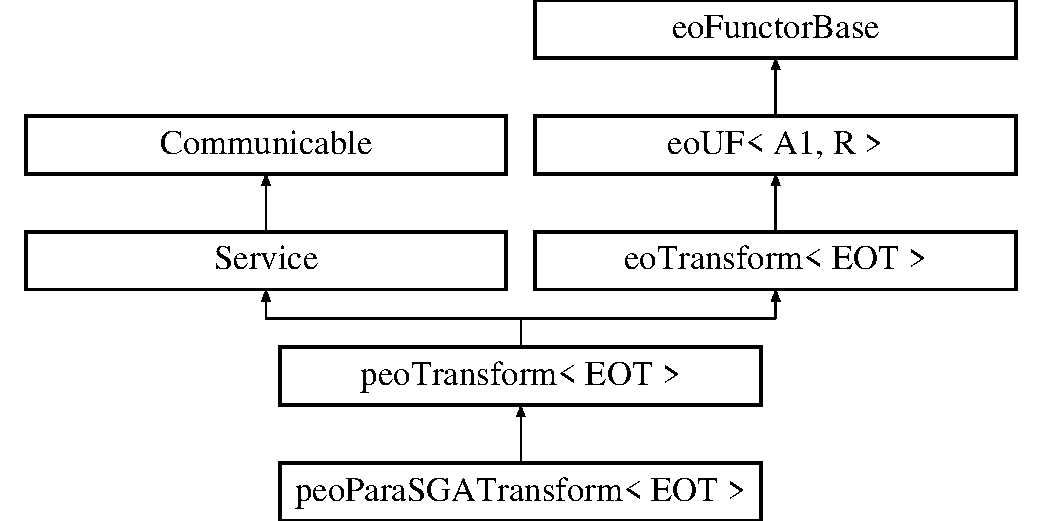
\includegraphics[height=4cm]{classpeoParaSGATransform}
\end{center}
\end{figure}
\subsection*{Public Member Functions}
\begin{CompactItemize}
\item 
\hypertarget{classpeoParaSGATransform_2052bca82fbbfe5455bf6f69246d4dbf}{
\hyperlink{classpeoParaSGATransform_2052bca82fbbfe5455bf6f69246d4dbf}{peo\-Para\-SGATransform} (eo\-Quad\-Op$<$ EOT $>$ \&\_\-\_\-cross, double \_\-\_\-cross\_\-rate, eo\-Mon\-Op$<$ EOT $>$ \&\_\-\_\-mut, double \_\-\_\-mut\_\-rate)}
\label{classpeoParaSGATransform_2052bca82fbbfe5455bf6f69246d4dbf}

\item 
\hypertarget{classpeoParaSGATransform_669de7f7c6316fa745a15b909efb6527}{
void \hyperlink{classpeoParaSGATransform_669de7f7c6316fa745a15b909efb6527}{operator()} (eo\-Pop$<$ EOT $>$ \&\_\-\_\-pop)}
\label{classpeoParaSGATransform_669de7f7c6316fa745a15b909efb6527}

\item 
\hypertarget{classpeoParaSGATransform_fd278bcde58d29c9a343d5cbead81a1e}{
void \hyperlink{classpeoParaSGATransform_fd278bcde58d29c9a343d5cbead81a1e}{pack\-Data} ()}
\label{classpeoParaSGATransform_fd278bcde58d29c9a343d5cbead81a1e}

\item 
\hypertarget{classpeoParaSGATransform_a43a487a6e81791c8bbf6ce30f4336ab}{
void \hyperlink{classpeoParaSGATransform_a43a487a6e81791c8bbf6ce30f4336ab}{unpack\-Data} ()}
\label{classpeoParaSGATransform_a43a487a6e81791c8bbf6ce30f4336ab}

\item 
\hypertarget{classpeoParaSGATransform_c9de2100fb897177a401c634002f6dd9}{
void \hyperlink{classpeoParaSGATransform_c9de2100fb897177a401c634002f6dd9}{execute} ()}
\label{classpeoParaSGATransform_c9de2100fb897177a401c634002f6dd9}

\item 
\hypertarget{classpeoParaSGATransform_ba08e224ceaa4149e8e1a88694a2ccf2}{
void \hyperlink{classpeoParaSGATransform_ba08e224ceaa4149e8e1a88694a2ccf2}{pack\-Result} ()}
\label{classpeoParaSGATransform_ba08e224ceaa4149e8e1a88694a2ccf2}

\item 
\hypertarget{classpeoParaSGATransform_257663dcdc6cc95b6183d472ffba1b2f}{
void \hyperlink{classpeoParaSGATransform_257663dcdc6cc95b6183d472ffba1b2f}{unpack\-Result} ()}
\label{classpeoParaSGATransform_257663dcdc6cc95b6183d472ffba1b2f}

\item 
\hypertarget{classpeoParaSGATransform_4e19dfc22b6f69fa8b93537226551866}{
void \hyperlink{classpeoParaSGATransform_4e19dfc22b6f69fa8b93537226551866}{notify\-Sending\-Data} ()}
\label{classpeoParaSGATransform_4e19dfc22b6f69fa8b93537226551866}

\item 
\hypertarget{classpeoParaSGATransform_8a0316e33897c395a81787f59ea7a1c8}{
void \hyperlink{classpeoParaSGATransform_8a0316e33897c395a81787f59ea7a1c8}{notify\-Sending\-All\-Resource\-Requests} ()}
\label{classpeoParaSGATransform_8a0316e33897c395a81787f59ea7a1c8}

\end{CompactItemize}
\subsection*{Private Attributes}
\begin{CompactItemize}
\item 
\hypertarget{classpeoParaSGATransform_c6f97deabe7502c84f5b6c479013f6dc}{
eo\-Quad\-Op$<$ EOT $>$ \& \hyperlink{classpeoParaSGATransform_c6f97deabe7502c84f5b6c479013f6dc}{cross}}
\label{classpeoParaSGATransform_c6f97deabe7502c84f5b6c479013f6dc}

\item 
\hypertarget{classpeoParaSGATransform_dfcf216e2df05016db4d57a5ffb0b0e2}{
double \hyperlink{classpeoParaSGATransform_dfcf216e2df05016db4d57a5ffb0b0e2}{cross\_\-rate}}
\label{classpeoParaSGATransform_dfcf216e2df05016db4d57a5ffb0b0e2}

\item 
\hypertarget{classpeoParaSGATransform_34ff5f9d285ca4879cf8865fb425a311}{
eo\-Mon\-Op$<$ EOT $>$ \& \hyperlink{classpeoParaSGATransform_34ff5f9d285ca4879cf8865fb425a311}{mut}}
\label{classpeoParaSGATransform_34ff5f9d285ca4879cf8865fb425a311}

\item 
\hypertarget{classpeoParaSGATransform_b9d3a2094737d0bbd034aac942cc53e3}{
double \hyperlink{classpeoParaSGATransform_b9d3a2094737d0bbd034aac942cc53e3}{mut\_\-rate}}
\label{classpeoParaSGATransform_b9d3a2094737d0bbd034aac942cc53e3}

\item 
\hypertarget{classpeoParaSGATransform_03972feadc86626e58fe60bd4061b57e}{
unsigned \hyperlink{classpeoParaSGATransform_03972feadc86626e58fe60bd4061b57e}{idx}}
\label{classpeoParaSGATransform_03972feadc86626e58fe60bd4061b57e}

\item 
\hypertarget{classpeoParaSGATransform_94e10a1285e128aba6e71517c941f961}{
eo\-Pop$<$ EOT $>$ $\ast$ \hyperlink{classpeoParaSGATransform_94e10a1285e128aba6e71517c941f961}{pop}}
\label{classpeoParaSGATransform_94e10a1285e128aba6e71517c941f961}

\item 
\hypertarget{classpeoParaSGATransform_9ef60190e2e3bd5961a93d1b52cb275d}{
EOT \hyperlink{classpeoParaSGATransform_9ef60190e2e3bd5961a93d1b52cb275d}{father}}
\label{classpeoParaSGATransform_9ef60190e2e3bd5961a93d1b52cb275d}

\item 
\hypertarget{classpeoParaSGATransform_e991ad2af6d116afd855de2db46e1d27}{
EOT \hyperlink{classpeoParaSGATransform_e991ad2af6d116afd855de2db46e1d27}{mother}}
\label{classpeoParaSGATransform_e991ad2af6d116afd855de2db46e1d27}

\item 
\hypertarget{classpeoParaSGATransform_589ea7cd72d522ae51a07de4d8ffbf11}{
unsigned \hyperlink{classpeoParaSGATransform_589ea7cd72d522ae51a07de4d8ffbf11}{num\_\-term}}
\label{classpeoParaSGATransform_589ea7cd72d522ae51a07de4d8ffbf11}

\end{CompactItemize}


\subsection{Detailed Description}
\subsubsection*{template$<$class EOT$>$ class peo\-Para\-SGATransform$<$ EOT $>$}





Definition at line 36 of file peo\-Para\-SGATransform.h.

The documentation for this class was generated from the following file:\begin{CompactItemize}
\item 
peo\-Para\-SGATransform.h\end{CompactItemize}

\hypertarget{classpeoPopEval}{
\section{peo\-Pop\-Eval$<$ EOT $>$ Class Template Reference}
\label{classpeoPopEval}\index{peoPopEval@{peoPopEval}}
}
The {\bf \hyperlink{classpeoPopEval}{peo\-Pop\-Eval}} class provides the interface for constructing Paradis\-EO specific evaluation functors.  


{\tt \#include $<$peo\-Pop\-Eval.h$>$}

Inheritance diagram for peo\-Pop\-Eval$<$ EOT $>$::\begin{figure}[H]
\begin{center}
\leavevmode
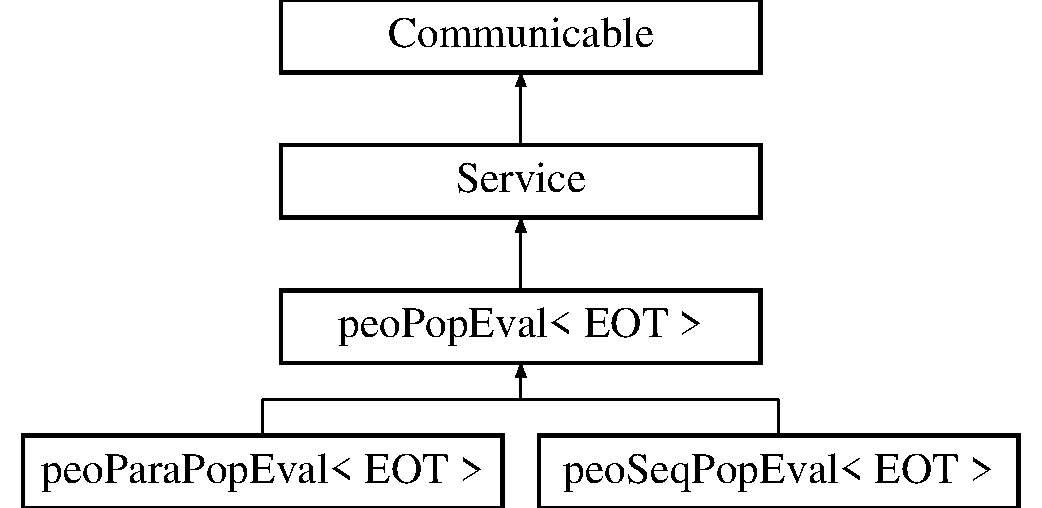
\includegraphics[height=4cm]{classpeoPopEval}
\end{center}
\end{figure}
\subsection*{Public Member Functions}
\begin{CompactItemize}
\item 
\hypertarget{classpeoPopEval_2f208067a5e39c3b26c1234050a41e8f}{
virtual void \hyperlink{classpeoPopEval_2f208067a5e39c3b26c1234050a41e8f}{operator()} (eo\-Pop$<$ EOT $>$ \&\_\-\_\-pop)=0}
\label{classpeoPopEval_2f208067a5e39c3b26c1234050a41e8f}

\begin{CompactList}\small\item\em Interface function providing the signature for constructing an evaluation functor. \item\end{CompactList}\end{CompactItemize}


\subsection{Detailed Description}
\subsubsection*{template$<$class EOT$>$ class peo\-Pop\-Eval$<$ EOT $>$}

The {\bf \hyperlink{classpeoPopEval}{peo\-Pop\-Eval}} class provides the interface for constructing Paradis\-EO specific evaluation functors. 

The derived classes may be used as wrappers for {\bf EO}-derived evaluation functors. In order to have an example, please refer to the implementation of the {\bf \hyperlink{classpeoSeqPopEval}{peo\-Seq\-Pop\-Eval}} and {\bf \hyperlink{classpeoParaPopEval}{peo\-Para\-Pop\-Eval}} classes. 



Definition at line 34 of file peo\-Pop\-Eval.h.

The documentation for this class was generated from the following file:\begin{CompactItemize}
\item 
peo\-Pop\-Eval.h\end{CompactItemize}

\hypertarget{classpeoSeqPopEval}{
\section{peo\-Seq\-Pop\-Eval$<$ EOT $>$ Class Template Reference}
\label{classpeoSeqPopEval}\index{peoSeqPopEval@{peoSeqPopEval}}
}
The \hyperlink{classpeoSeqPopEval}{peo\-Seq\-Pop\-Eval} class acts only as a Paradis\-EO specific sequential evaluation functor - a wrapper for incorporating an {\bf eo\-Eval\-Func$<$ EOT $>$}-derived class as evaluation functor.  


{\tt \#include $<$peo\-Seq\-Pop\-Eval.h$>$}

Inheritance diagram for peo\-Seq\-Pop\-Eval$<$ EOT $>$::\begin{figure}[H]
\begin{center}
\leavevmode
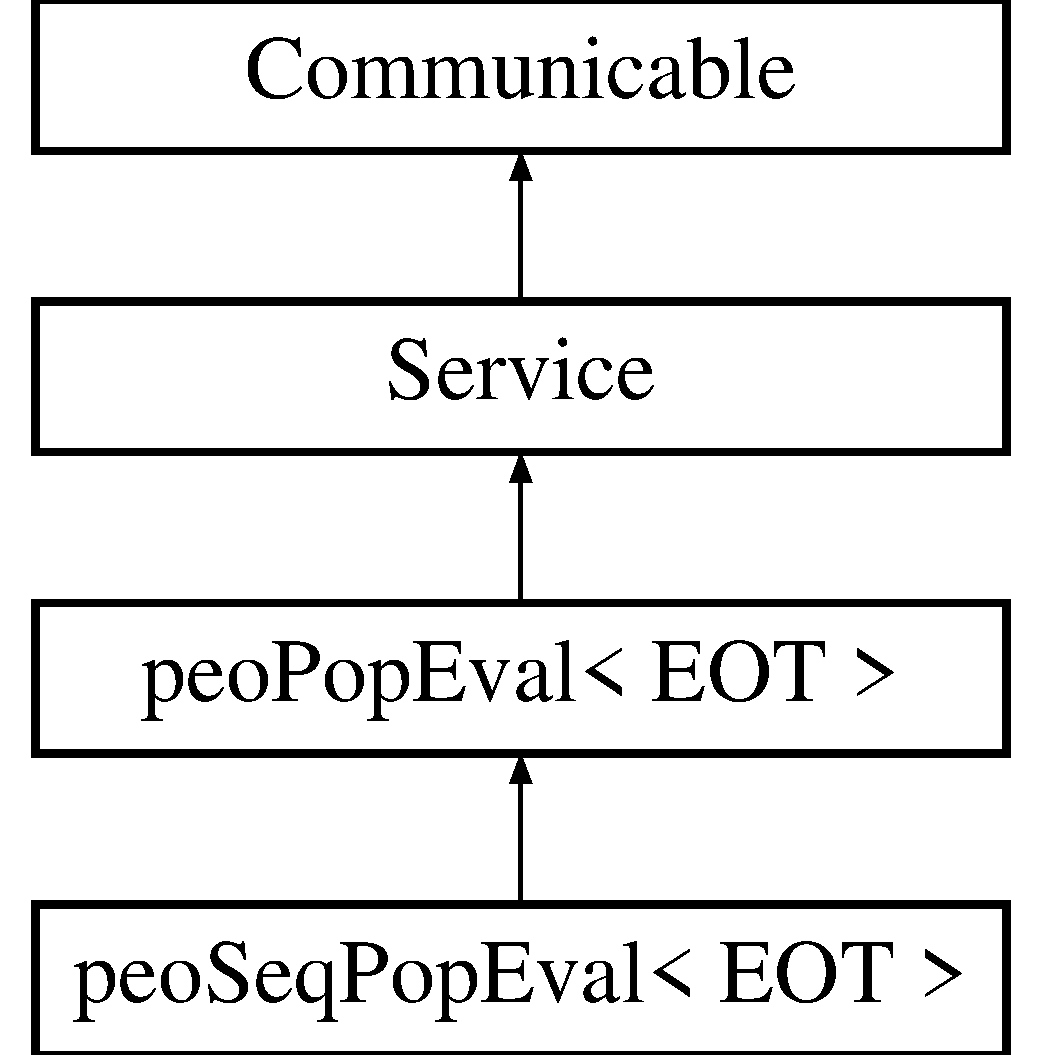
\includegraphics[height=4cm]{classpeoSeqPopEval}
\end{center}
\end{figure}
\subsection*{Public Member Functions}
\begin{CompactItemize}
\item 
\hyperlink{classpeoSeqPopEval_a41f91ab4b2aeb325ff75feb66d4e003}{peo\-Seq\-Pop\-Eval} (eo\-Eval\-Func$<$ EOT $>$ \&\_\-\_\-eval)
\begin{CompactList}\small\item\em Constructor function - it only sets an internal reference to point to the specified evaluation object. \item\end{CompactList}\item 
void \hyperlink{classpeoSeqPopEval_b2c88b9a3ad9091949acf741844eb02f}{operator()} (eo\-Pop$<$ EOT $>$ \&\_\-\_\-pop)
\begin{CompactList}\small\item\em Operator for evaluating all the individuals of a given population - in a sequential iterative manner. \item\end{CompactList}\end{CompactItemize}
\subsection*{Private Attributes}
\begin{CompactItemize}
\item 
\hypertarget{classpeoSeqPopEval_5465f31386c6b96bc8f7fb9393a28a2f}{
eo\-Eval\-Func$<$ EOT $>$ \& \hyperlink{classpeoSeqPopEval_5465f31386c6b96bc8f7fb9393a28a2f}{eval}}
\label{classpeoSeqPopEval_5465f31386c6b96bc8f7fb9393a28a2f}

\end{CompactItemize}


\subsection{Detailed Description}
\subsubsection*{template$<$class EOT$>$ class peo\-Seq\-Pop\-Eval$<$ EOT $>$}

The \hyperlink{classpeoSeqPopEval}{peo\-Seq\-Pop\-Eval} class acts only as a Paradis\-EO specific sequential evaluation functor - a wrapper for incorporating an {\bf eo\-Eval\-Func$<$ EOT $>$}-derived class as evaluation functor. 

The specified EO evaluation object is applyied in an iterative manner to each individual of a specified population. 



Definition at line 21 of file peo\-Seq\-Pop\-Eval.h.

\subsection{Constructor \& Destructor Documentation}
\hypertarget{classpeoSeqPopEval_a41f91ab4b2aeb325ff75feb66d4e003}{
\index{peoSeqPopEval@{peo\-Seq\-Pop\-Eval}!peoSeqPopEval@{peoSeqPopEval}}
\index{peoSeqPopEval@{peoSeqPopEval}!peoSeqPopEval@{peo\-Seq\-Pop\-Eval}}
\subsubsection[peoSeqPopEval]{\setlength{\rightskip}{0pt plus 5cm}template$<$class EOT$>$ \hyperlink{classpeoSeqPopEval}{peo\-Seq\-Pop\-Eval}$<$ EOT $>$::\hyperlink{classpeoSeqPopEval}{peo\-Seq\-Pop\-Eval} (eo\-Eval\-Func$<$ EOT $>$ \& {\em \_\-\_\-eval})}}
\label{classpeoSeqPopEval_a41f91ab4b2aeb325ff75feb66d4e003}


Constructor function - it only sets an internal reference to point to the specified evaluation object. 

\begin{Desc}
\item[Parameters:]
\begin{description}
\item[{\em eo\-Eval\-Func$<$}]EOT $>$\& \_\-\_\-eval - evaluation object to be applied for each individual of a specified population \end{description}
\end{Desc}


Definition at line 41 of file peo\-Seq\-Pop\-Eval.h.

\subsection{Member Function Documentation}
\hypertarget{classpeoSeqPopEval_b2c88b9a3ad9091949acf741844eb02f}{
\index{peoSeqPopEval@{peo\-Seq\-Pop\-Eval}!operator()@{operator()}}
\index{operator()@{operator()}!peoSeqPopEval@{peo\-Seq\-Pop\-Eval}}
\subsubsection[operator()]{\setlength{\rightskip}{0pt plus 5cm}template$<$class EOT$>$ void \hyperlink{classpeoSeqPopEval}{peo\-Seq\-Pop\-Eval}$<$ EOT $>$::operator() (eo\-Pop$<$ EOT $>$ \& {\em \_\-\_\-pop})\hspace{0.3cm}{\tt  \mbox{[}virtual\mbox{]}}}}
\label{classpeoSeqPopEval_b2c88b9a3ad9091949acf741844eb02f}


Operator for evaluating all the individuals of a given population - in a sequential iterative manner. 

\begin{Desc}
\item[Parameters:]
\begin{description}
\item[{\em eo\-Pop$<$}]EOT $>$\& \_\-\_\-pop - population to be evaluated. \end{description}
\end{Desc}


Implements \hyperlink{classpeoPopEval_2f208067a5e39c3b26c1234050a41e8f}{peo\-Pop\-Eval$<$ EOT $>$}.

Definition at line 46 of file peo\-Seq\-Pop\-Eval.h.

References peo\-Seq\-Pop\-Eval$<$ EOT $>$::eval.

The documentation for this class was generated from the following file:\begin{CompactItemize}
\item 
peo\-Seq\-Pop\-Eval.h\end{CompactItemize}

\hypertarget{classpeoSeqTransform}{
\section{peo\-Seq\-Transform$<$ EOT $>$ Class Template Reference}
\label{classpeoSeqTransform}\index{peoSeqTransform@{peoSeqTransform}}
}
The \hyperlink{classpeoSeqTransform}{peo\-Seq\-Transform} represent a wrapper for offering the possibility of using \doxyref{EO} derived transform operators along with the Paradis\-EO evolutionary algorithms.  


{\tt \#include $<$peo\-Seq\-Transform.h$>$}

Inheritance diagram for peo\-Seq\-Transform$<$ EOT $>$::\begin{figure}[H]
\begin{center}
\leavevmode
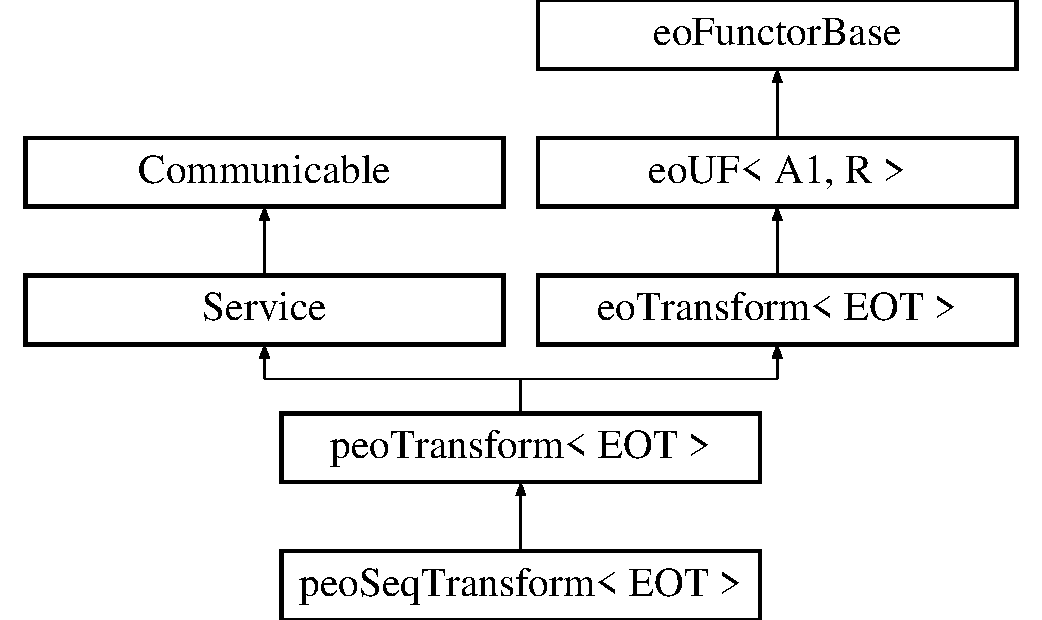
\includegraphics[height=5cm]{classpeoSeqTransform}
\end{center}
\end{figure}
\subsection*{Public Member Functions}
\begin{CompactItemize}
\item 
\hyperlink{classpeoSeqTransform_3b8e4ed19d9458938eb669d83a53c626}{peo\-Seq\-Transform} (\bf{eo\-Transform}$<$ EOT $>$ \&\_\-\_\-trans)
\begin{CompactList}\small\item\em Constructor function - sets an internal reference towards the specified EO-derived transform object. \item\end{CompactList}\item 
void \hyperlink{classpeoSeqTransform_1ba63536abb6c4e1c369e0b7e066872e}{operator()} (\bf{eo\-Pop}$<$ EOT $>$ \&\_\-\_\-pop)
\begin{CompactList}\small\item\em Operator for applying the specified transform operators on each individual of the given population. \item\end{CompactList}\item 
\hypertarget{classpeoSeqTransform_c4bf2724e9f6055f12bd169fad893be3}{
virtual void \hyperlink{classpeoSeqTransform_c4bf2724e9f6055f12bd169fad893be3}{pack\-Data} ()}
\label{classpeoSeqTransform_c4bf2724e9f6055f12bd169fad893be3}

\begin{CompactList}\small\item\em Interface function for providing a link with the parallel architecture of the Paradis\-EO framework. \item\end{CompactList}\item 
\hypertarget{classpeoSeqTransform_24e6cf15ef230ed538031b522ddd4ae6}{
virtual void \hyperlink{classpeoSeqTransform_24e6cf15ef230ed538031b522ddd4ae6}{unpack\-Data} ()}
\label{classpeoSeqTransform_24e6cf15ef230ed538031b522ddd4ae6}

\begin{CompactList}\small\item\em Interface function for providing a link with the parallel architecture of the Paradis\-EO framework. \item\end{CompactList}\item 
\hypertarget{classpeoSeqTransform_0294a2f9d6b44ec74d22eaceccdffc2b}{
virtual void \hyperlink{classpeoSeqTransform_0294a2f9d6b44ec74d22eaceccdffc2b}{execute} ()}
\label{classpeoSeqTransform_0294a2f9d6b44ec74d22eaceccdffc2b}

\begin{CompactList}\small\item\em Interface function for providing a link with the parallel architecture of the Paradis\-EO framework. \item\end{CompactList}\item 
\hypertarget{classpeoSeqTransform_4861c61f9e46d83964ea8a156a9a3ee0}{
virtual void \hyperlink{classpeoSeqTransform_4861c61f9e46d83964ea8a156a9a3ee0}{pack\-Result} ()}
\label{classpeoSeqTransform_4861c61f9e46d83964ea8a156a9a3ee0}

\begin{CompactList}\small\item\em Interface function for providing a link with the parallel architecture of the Paradis\-EO framework. \item\end{CompactList}\item 
\hypertarget{classpeoSeqTransform_5dd029fc011eb2a810ca1140025129b1}{
virtual void \hyperlink{classpeoSeqTransform_5dd029fc011eb2a810ca1140025129b1}{unpack\-Result} ()}
\label{classpeoSeqTransform_5dd029fc011eb2a810ca1140025129b1}

\begin{CompactList}\small\item\em Interface function for providing a link with the parallel architecture of the Paradis\-EO framework. \item\end{CompactList}\end{CompactItemize}
\subsection*{Private Attributes}
\begin{CompactItemize}
\item 
\hypertarget{classpeoSeqTransform_ad3e16c59dd6c46dfc1baf7b88af30cf}{
\bf{eo\-Transform}$<$ EOT $>$ \& \hyperlink{classpeoSeqTransform_ad3e16c59dd6c46dfc1baf7b88af30cf}{trans}}
\label{classpeoSeqTransform_ad3e16c59dd6c46dfc1baf7b88af30cf}

\end{CompactItemize}


\subsection{Detailed Description}
\subsubsection*{template$<$class EOT$>$ class peo\-Seq\-Transform$<$ EOT $>$}

The \hyperlink{classpeoSeqTransform}{peo\-Seq\-Transform} represent a wrapper for offering the possibility of using \doxyref{EO} derived transform operators along with the Paradis\-EO evolutionary algorithms. 

A minimal set of interface functions is also provided for creating the link with the parallel architecture of the Paradis\-EO framework. 



Definition at line 48 of file peo\-Seq\-Transform.h.

\subsection{Constructor \& Destructor Documentation}
\hypertarget{classpeoSeqTransform_3b8e4ed19d9458938eb669d83a53c626}{
\index{peoSeqTransform@{peo\-Seq\-Transform}!peoSeqTransform@{peoSeqTransform}}
\index{peoSeqTransform@{peoSeqTransform}!peoSeqTransform@{peo\-Seq\-Transform}}
\subsubsection[peoSeqTransform]{\setlength{\rightskip}{0pt plus 5cm}template$<$class EOT$>$ \hyperlink{classpeoSeqTransform}{peo\-Seq\-Transform}$<$ EOT $>$::\hyperlink{classpeoSeqTransform}{peo\-Seq\-Transform} (\bf{eo\-Transform}$<$ EOT $>$ \& {\em \_\-\_\-trans})}}
\label{classpeoSeqTransform_3b8e4ed19d9458938eb669d83a53c626}


Constructor function - sets an internal reference towards the specified EO-derived transform object. 

\begin{Desc}
\item[Parameters:]
\begin{description}
\item[{\em eo\-Transform$<$}]EOT $>$\& \_\-\_\-trans - EO-derived transform object including crossover and mutation operators. \end{description}
\end{Desc}


Definition at line 83 of file peo\-Seq\-Transform.h.

\subsection{Member Function Documentation}
\hypertarget{classpeoSeqTransform_1ba63536abb6c4e1c369e0b7e066872e}{
\index{peoSeqTransform@{peo\-Seq\-Transform}!operator()@{operator()}}
\index{operator()@{operator()}!peoSeqTransform@{peo\-Seq\-Transform}}
\subsubsection[operator()]{\setlength{\rightskip}{0pt plus 5cm}template$<$class EOT$>$ void \hyperlink{classpeoSeqTransform}{peo\-Seq\-Transform}$<$ EOT $>$::operator() (\bf{eo\-Pop}$<$ EOT $>$ \& {\em \_\-\_\-pop})}}
\label{classpeoSeqTransform_1ba63536abb6c4e1c369e0b7e066872e}


Operator for applying the specified transform operators on each individual of the given population. 

\begin{Desc}
\item[Parameters:]
\begin{description}
\item[{\em eo\-Pop$<$}]EOT $>$\& \_\-\_\-pop - population to be transformed by applying the crossover and mutation operators. \end{description}
\end{Desc}


Definition at line 88 of file peo\-Seq\-Transform.h.

References peo\-Seq\-Transform$<$ EOT $>$::trans.

The documentation for this class was generated from the following file:\begin{CompactItemize}
\item 
peo\-Seq\-Transform.h\end{CompactItemize}

\hypertarget{classpeoSyncIslandMig}{
\section{peo\-Sync\-Island\-Mig$<$ TYPESELECT, TYPEREPLACE $>$ Class Template Reference}
\label{classpeoSyncIslandMig}\index{peoSyncIslandMig@{peoSyncIslandMig}}
}
Specific class for a synchronous migration.  


{\tt \#include $<$peo\-Sync\-Island\-Mig.h$>$}

Inheritance diagram for peo\-Sync\-Island\-Mig$<$ TYPESELECT, TYPEREPLACE $>$::\begin{figure}[H]
\begin{center}
\leavevmode
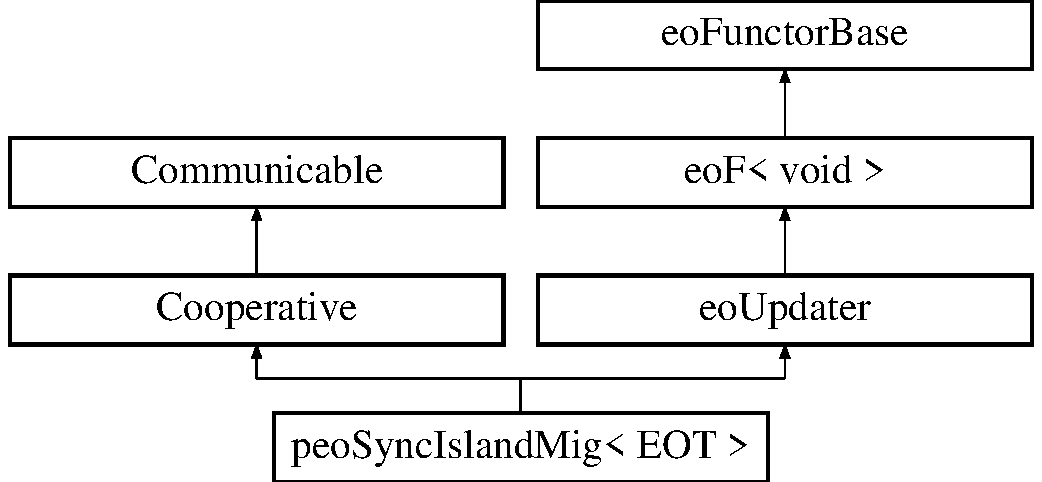
\includegraphics[height=3.44615cm]{classpeoSyncIslandMig}
\end{center}
\end{figure}
\subsection*{Public Member Functions}
\begin{CompactItemize}
\item 
\hyperlink{classpeoSyncIslandMig_24f4d1ea8bb63c09b9d6cd8476014082}{peo\-Sync\-Island\-Mig} (unsigned \_\-\_\-frequency, \hyperlink{classselector}{selector}$<$ TYPESELECT $>$ \&\_\-\_\-select, \hyperlink{classreplacement}{replacement}$<$ TYPEREPLACE $>$ \&\_\-\_\-replace, \hyperlink{classTopology}{Topology} \&\_\-\_\-topology)
\item 
\hypertarget{classpeoSyncIslandMig_0fd5b3b4e467ee33ae0186c0ae9d58ef}{
void \hyperlink{classpeoSyncIslandMig_0fd5b3b4e467ee33ae0186c0ae9d58ef}{operator()} ()}
\label{classpeoSyncIslandMig_0fd5b3b4e467ee33ae0186c0ae9d58ef}

\begin{CompactList}\small\item\em operator \item\end{CompactList}\item 
\hypertarget{classpeoSyncIslandMig_2daadf9928b8075ea469ca3cc49ddc88}{
void \hyperlink{classpeoSyncIslandMig_2daadf9928b8075ea469ca3cc49ddc88}{pack} ()}
\label{classpeoSyncIslandMig_2daadf9928b8075ea469ca3cc49ddc88}

\begin{CompactList}\small\item\em \doxyref{Function} realizing packages. \item\end{CompactList}\item 
\hypertarget{classpeoSyncIslandMig_25bc1a03cc49e17dda34b6647df1f9c5}{
void \hyperlink{classpeoSyncIslandMig_25bc1a03cc49e17dda34b6647df1f9c5}{unpack} ()}
\label{classpeoSyncIslandMig_25bc1a03cc49e17dda34b6647df1f9c5}

\begin{CompactList}\small\item\em \doxyref{Function} reconstituting packages. \item\end{CompactList}\item 
\hypertarget{classpeoSyncIslandMig_956f56110bccff8c8fae4b05aa804d32}{
void \hyperlink{classpeoSyncIslandMig_956f56110bccff8c8fae4b05aa804d32}{pack\-Synchronize\-Req} ()}
\label{classpeoSyncIslandMig_956f56110bccff8c8fae4b05aa804d32}

\begin{CompactList}\small\item\em \doxyref{Function} pack\-Synchronize\-Req. \item\end{CompactList}\item 
\hypertarget{classpeoSyncIslandMig_5f403428cea887b07caf27ab265ebe03}{
void \hyperlink{classpeoSyncIslandMig_5f403428cea887b07caf27ab265ebe03}{notify\-Sending} ()}
\label{classpeoSyncIslandMig_5f403428cea887b07caf27ab265ebe03}

\begin{CompactList}\small\item\em \doxyref{Function} notify\-Sending. \item\end{CompactList}\item 
\hypertarget{classpeoSyncIslandMig_75aacd3f7ffbc302c69addc342f45b8f}{
void \hyperlink{classpeoSyncIslandMig_75aacd3f7ffbc302c69addc342f45b8f}{notify\-Receiving} ()}
\label{classpeoSyncIslandMig_75aacd3f7ffbc302c69addc342f45b8f}

\begin{CompactList}\small\item\em \doxyref{Function} notify\-Receiving. \item\end{CompactList}\item 
\hypertarget{classpeoSyncIslandMig_92fef53496f935fe450589f90aec7d72}{
void \hyperlink{classpeoSyncIslandMig_92fef53496f935fe450589f90aec7d72}{notify\-Sending\-Sync\-Req} ()}
\label{classpeoSyncIslandMig_92fef53496f935fe450589f90aec7d72}

\begin{CompactList}\small\item\em notify\-Sending\-Sync\-Req \item\end{CompactList}\item 
\hypertarget{classpeoSyncIslandMig_0abd0c5872195cea0cab4988f9a4ea4e}{
void \hyperlink{classpeoSyncIslandMig_0abd0c5872195cea0cab4988f9a4ea4e}{notify\-Synchronized} ()}
\label{classpeoSyncIslandMig_0abd0c5872195cea0cab4988f9a4ea4e}

\begin{CompactList}\small\item\em notify\-Synchronized \item\end{CompactList}\end{CompactItemize}
\subsection*{Private Member Functions}
\begin{CompactItemize}
\item 
\hypertarget{classpeoSyncIslandMig_3ab202cb311f67fdc827078b3bdfddf4}{
void \hyperlink{classpeoSyncIslandMig_3ab202cb311f67fdc827078b3bdfddf4}{emigrate} ()}
\label{classpeoSyncIslandMig_3ab202cb311f67fdc827078b3bdfddf4}

\item 
\hypertarget{classpeoSyncIslandMig_baed2215bf06f96aacf06b5abff79f28}{
void \hyperlink{classpeoSyncIslandMig_baed2215bf06f96aacf06b5abff79f28}{immigrate} ()}
\label{classpeoSyncIslandMig_baed2215bf06f96aacf06b5abff79f28}

\end{CompactItemize}
\subsection*{Private Attributes}
\begin{CompactItemize}
\item 
\hyperlink{classeoSyncContinue}{eo\-Sync\-Continue} \hyperlink{classpeoSyncIslandMig_a64e7c9da149773c5d264d128a1ea37a}{cont}
\item 
\hypertarget{classpeoSyncIslandMig_a399c2533598dc8018eb2ab2edabd6b9}{
\hyperlink{classselector}{selector}$<$ TYPESELECT $>$ \& \hyperlink{classpeoSyncIslandMig_a399c2533598dc8018eb2ab2edabd6b9}{select}}
\label{classpeoSyncIslandMig_a399c2533598dc8018eb2ab2edabd6b9}

\item 
\hypertarget{classpeoSyncIslandMig_34b69e0a2fa12ef0f6101c7d04ebc3ef}{
\hyperlink{classreplacement}{replacement}$<$ TYPEREPLACE $>$ \& \hyperlink{classpeoSyncIslandMig_34b69e0a2fa12ef0f6101c7d04ebc3ef}{replace}}
\label{classpeoSyncIslandMig_34b69e0a2fa12ef0f6101c7d04ebc3ef}

\item 
\hypertarget{classpeoSyncIslandMig_7376532c3a8bcab88a02601611db9f2f}{
\hyperlink{classTopology}{Topology} \& \hyperlink{classpeoSyncIslandMig_7376532c3a8bcab88a02601611db9f2f}{topology}}
\label{classpeoSyncIslandMig_7376532c3a8bcab88a02601611db9f2f}

\item 
\hypertarget{classpeoSyncIslandMig_4c734df065099cfd5693d35fae38ad29}{
std::queue$<$ TYPEREPLACE $>$ \hyperlink{classpeoSyncIslandMig_4c734df065099cfd5693d35fae38ad29}{imm}}
\label{classpeoSyncIslandMig_4c734df065099cfd5693d35fae38ad29}

\item 
\hypertarget{classpeoSyncIslandMig_b96f8caff26498798eb0e4c114ee5d9a}{
std::queue$<$ TYPESELECT $>$ \hyperlink{classpeoSyncIslandMig_b96f8caff26498798eb0e4c114ee5d9a}{em}}
\label{classpeoSyncIslandMig_b96f8caff26498798eb0e4c114ee5d9a}

\item 
\hypertarget{classpeoSyncIslandMig_ad56e3475d8ea7a83007c2e32c7da6a8}{
std::queue$<$ \hyperlink{classCooperative}{Cooperative} $\ast$ $>$ \hyperlink{classpeoSyncIslandMig_ad56e3475d8ea7a83007c2e32c7da6a8}{coop\_\-em}}
\label{classpeoSyncIslandMig_ad56e3475d8ea7a83007c2e32c7da6a8}

\item 
\hypertarget{classpeoSyncIslandMig_9431b7e1d629f238cd5f990d02926480}{
sem\_\-t \hyperlink{classpeoSyncIslandMig_9431b7e1d629f238cd5f990d02926480}{sync}}
\label{classpeoSyncIslandMig_9431b7e1d629f238cd5f990d02926480}

\item 
\hypertarget{classpeoSyncIslandMig_253dfbfebfadad0b4f49e60bb811b1db}{
bool \hyperlink{classpeoSyncIslandMig_253dfbfebfadad0b4f49e60bb811b1db}{explicit\-Passive}}
\label{classpeoSyncIslandMig_253dfbfebfadad0b4f49e60bb811b1db}

\item 
\hypertarget{classpeoSyncIslandMig_e5d64ff9718b746d2307379fb061ad96}{
bool \hyperlink{classpeoSyncIslandMig_e5d64ff9718b746d2307379fb061ad96}{standby\-Migration}}
\label{classpeoSyncIslandMig_e5d64ff9718b746d2307379fb061ad96}

\item 
\hypertarget{classpeoSyncIslandMig_6274e5185b6b7579dea71da3138d9d23}{
std::vector$<$ \hyperlink{classCooperative}{Cooperative} $\ast$ $>$ \hyperlink{classpeoSyncIslandMig_6274e5185b6b7579dea71da3138d9d23}{in}}
\label{classpeoSyncIslandMig_6274e5185b6b7579dea71da3138d9d23}

\item 
\hypertarget{classpeoSyncIslandMig_daae2fea2f447d35927e18a8f008a45d}{
std::vector$<$ \hyperlink{classCooperative}{Cooperative} $\ast$ $>$ \hyperlink{classpeoSyncIslandMig_daae2fea2f447d35927e18a8f008a45d}{out}}
\label{classpeoSyncIslandMig_daae2fea2f447d35927e18a8f008a45d}

\item 
\hypertarget{classpeoSyncIslandMig_2760dde833d7141ca86affb4df0fb163}{
std::vector$<$ \hyperlink{classCooperative}{Cooperative} $\ast$ $>$ \hyperlink{classpeoSyncIslandMig_2760dde833d7141ca86affb4df0fb163}{all}}
\label{classpeoSyncIslandMig_2760dde833d7141ca86affb4df0fb163}

\item 
\hypertarget{classpeoSyncIslandMig_cdd55a0ab14d659a2a68674a05ed8a1d}{
unsigned \hyperlink{classpeoSyncIslandMig_cdd55a0ab14d659a2a68674a05ed8a1d}{nb\-Migrations}}
\label{classpeoSyncIslandMig_cdd55a0ab14d659a2a68674a05ed8a1d}

\end{CompactItemize}


\subsection{Detailed Description}
\subsubsection*{template$<$class TYPESELECT, class TYPEREPLACE$>$ class peo\-Sync\-Island\-Mig$<$ TYPESELECT, TYPEREPLACE $>$}

Specific class for a synchronous migration. 

\begin{Desc}
\item[See also:]\hyperlink{classCooperative}{Cooperative} \doxyref{eo\-Updater} \end{Desc}
\begin{Desc}
\item[Version:]2.0 \end{Desc}
\begin{Desc}
\item[Date:]january 2008 \end{Desc}




Definition at line 71 of file peo\-Sync\-Island\-Mig.h.

\subsection{Constructor \& Destructor Documentation}
\hypertarget{classpeoSyncIslandMig_24f4d1ea8bb63c09b9d6cd8476014082}{
\index{peoSyncIslandMig@{peo\-Sync\-Island\-Mig}!peoSyncIslandMig@{peoSyncIslandMig}}
\index{peoSyncIslandMig@{peoSyncIslandMig}!peoSyncIslandMig@{peo\-Sync\-Island\-Mig}}
\subsubsection[peoSyncIslandMig]{\setlength{\rightskip}{0pt plus 5cm}template$<$class TYPESELECT, class TYPEREPLACE$>$ \hyperlink{classpeoSyncIslandMig}{peo\-Sync\-Island\-Mig}$<$ TYPESELECT, TYPEREPLACE $>$::\hyperlink{classpeoSyncIslandMig}{peo\-Sync\-Island\-Mig} (unsigned {\em \_\-\_\-frequency}, \hyperlink{classselector}{selector}$<$ TYPESELECT $>$ \& {\em \_\-\_\-select}, \hyperlink{classreplacement}{replacement}$<$ TYPEREPLACE $>$ \& {\em \_\-\_\-replace}, \hyperlink{classTopology}{Topology} \& {\em \_\-\_\-topology})}}
\label{classpeoSyncIslandMig_24f4d1ea8bb63c09b9d6cd8476014082}


\begin{Desc}
\item[Parameters:]
\begin{description}
\item[{\em unsigned}]\_\-\_\-frequency \item[{\em selector}]$<$TYPESELECT$>$ \& \_\-\_\-select \item[{\em replacement}]$<$TYPEREPLACE$>$ \& \_\-\_\-replace \item[{\em Topology\&}]\_\-\_\-topology \end{description}
\end{Desc}


Definition at line 139 of file peo\-Sync\-Island\-Mig.h.

References Topology::add(), and peo\-Sync\-Island\-Mig$<$ TYPESELECT, TYPEREPLACE $>$::sync.

\subsection{Member Data Documentation}
\hypertarget{classpeoSyncIslandMig_a64e7c9da149773c5d264d128a1ea37a}{
\index{peoSyncIslandMig@{peo\-Sync\-Island\-Mig}!cont@{cont}}
\index{cont@{cont}!peoSyncIslandMig@{peo\-Sync\-Island\-Mig}}
\subsubsection[cont]{\setlength{\rightskip}{0pt plus 5cm}template$<$class TYPESELECT, class TYPEREPLACE$>$ \hyperlink{classeoSyncContinue}{eo\-Sync\-Continue} \hyperlink{classpeoSyncIslandMig}{peo\-Sync\-Island\-Mig}$<$ TYPESELECT, TYPEREPLACE $>$::\hyperlink{classpeoSyncIslandMig_a64e7c9da149773c5d264d128a1ea37a}{cont}\hspace{0.3cm}{\tt  \mbox{[}private\mbox{]}}}}
\label{classpeoSyncIslandMig_a64e7c9da149773c5d264d128a1ea37a}


\begin{Desc}
\item[Parameters:]
\begin{description}
\item[{\em \hyperlink{classeoSyncContinue}{eo\-Sync\-Continue}}]cont \item[{\em selector}]$<$TYPESELECT$>$ \& select \item[{\em replacement}]$<$TYPEREPLACE$>$ \& replace \item[{\em Topology\&}]topology \item[{\em std}]:: queue$<$ TYPEREPLACE $>$ imm \item[{\em std}]:: queue$<$ TYPESELECT $>$ em \item[{\em std}]:: queue$<$ Cooperative$\ast$ $>$ coop\_\-em \item[{\em sem\_\-t}]sync \item[{\em bool}]explicit\-Passive \item[{\em bool}]standby\-Migration \item[{\em std}]:: vector$<$ Cooperative$\ast$ $>$ in, out, all \item[{\em unsigned}]nb\-Migrations \end{description}
\end{Desc}


Definition at line 124 of file peo\-Sync\-Island\-Mig.h.

Referenced by peo\-Sync\-Island\-Mig$<$ TYPESELECT, TYPEREPLACE $>$::operator()().

The documentation for this class was generated from the following file:\begin{CompactItemize}
\item 
peo\-Sync\-Island\-Mig.h\end{CompactItemize}

\hypertarget{classpeoSyncMultiStart}{
\section{peo\-Sync\-Multi\-Start$<$ EOT $>$ Class Template Reference}
\label{classpeoSyncMultiStart}\index{peoSyncMultiStart@{peoSyncMultiStart}}
}
The \hyperlink{classpeoSyncMultiStart}{peo\-Sync\-Multi\-Start} class provides the basis for implementing the synchronous multi-start model, for launching several solution-based algorithms in parallel on a specified initial population.  


{\tt \#include $<$peo\-Sync\-Multi\-Start.h$>$}

Inheritance diagram for peo\-Sync\-Multi\-Start$<$ EOT $>$::\begin{figure}[H]
\begin{center}
\leavevmode
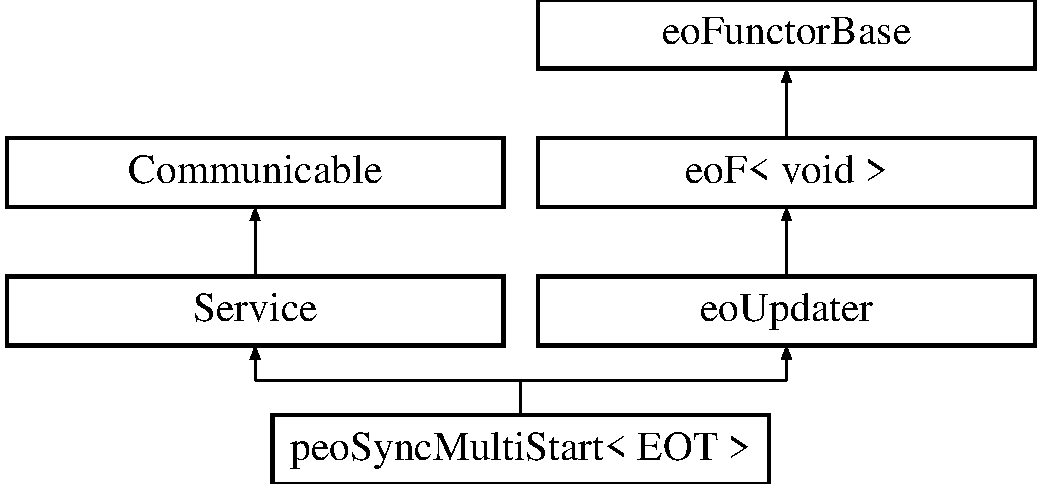
\includegraphics[height=4cm]{classpeoSyncMultiStart}
\end{center}
\end{figure}
\subsection*{Public Member Functions}
\begin{CompactItemize}
\item 
\hyperlink{classpeoSyncMultiStart_d29f94aad3c1f443bfffc8b6aee0704c}{peo\-Sync\-Multi\-Start} (\bf{eo\-Continue}$<$ EOT $>$ \&\_\-\_\-cont, \bf{eo\-Select}$<$ EOT $>$ \&\_\-\_\-select, \bf{eo\-Replacement}$<$ EOT $>$ \&\_\-\_\-replace, \bf{mo\-Algo}$<$ EOT $>$ \&\_\-\_\-ls, \bf{eo\-Pop}$<$ EOT $>$ \&\_\-\_\-pop)
\begin{CompactList}\small\item\em Constructor function - several simple parameters are required for defining the characteristics of the multi-start model. \item\end{CompactList}\item 
void \hyperlink{classpeoSyncMultiStart_76385b33fe514f91cb83f0fbecbeb3c2}{operator()} ()
\begin{CompactList}\small\item\em Operator which synchronously executes the specified algorithm on the individuals selected from the initial population. \item\end{CompactList}\item 
void \hyperlink{classpeoSyncMultiStart_8becfab1922b64708dca5a53e2932a5a}{pack\-Data} ()
\begin{CompactList}\small\item\em Auxiliary function for transferring data between the process requesting the synchronous execution of the specified algorithm and the process which actually executes the algorithm. \item\end{CompactList}\item 
void \hyperlink{classpeoSyncMultiStart_2903a441b77cded266b5fb651e17a5b5}{unpack\-Data} ()
\begin{CompactList}\small\item\em Auxiliary function for transferring data between the process requesting the synchronous execution of the specified algorithm and the process which actually executes the algorithm. \item\end{CompactList}\item 
void \hyperlink{classpeoSyncMultiStart_a4d1c2943c290de540800087b54dc49b}{execute} ()
\begin{CompactList}\small\item\em Auxiliary function for actually executing the specified algorithm on one assigned individual. \item\end{CompactList}\item 
void \hyperlink{classpeoSyncMultiStart_6c48eb0dae741cff7203b65e226f9616}{pack\-Result} ()
\begin{CompactList}\small\item\em Auxiliary function for transferring data between the process requesting the synchronous execution of the specified algorithm and the process which actually executes the algorithm. \item\end{CompactList}\item 
void \hyperlink{classpeoSyncMultiStart_c3cbd1f10a89d1915c5ccf82a2c34a1d}{unpack\-Result} ()
\begin{CompactList}\small\item\em Auxiliary function for transferring data between the process requesting the synchronous execution of the specified algorithm and the process which actually executes the algorithm. \item\end{CompactList}\item 
void \hyperlink{classpeoSyncMultiStart_32ec0d01d3fd8a9932abd68f4781fc94}{notify\-Sending\-Data} ()
\begin{CompactList}\small\item\em Auxiliary function for notifications between the process requesting the synchronous multi-start execution and the processes that performs the actual execution phase. \item\end{CompactList}\item 
void \hyperlink{classpeoSyncMultiStart_fc90282cc4e93cdea8f82fd52dd78fb0}{notify\-Sending\-All\-Resource\-Requests} ()
\begin{CompactList}\small\item\em Auxiliary function for notifications between the process requesting the synchronous multi-start execution and the processes that performs the actual execution phase. \item\end{CompactList}\end{CompactItemize}
\subsection*{Private Attributes}
\begin{CompactItemize}
\item 
\hypertarget{classpeoSyncMultiStart_43f4fa9b125baef6fc8b968dfd16f437}{
\bf{eo\-Continue}$<$ EOT $>$ \& \hyperlink{classpeoSyncMultiStart_43f4fa9b125baef6fc8b968dfd16f437}{cont}}
\label{classpeoSyncMultiStart_43f4fa9b125baef6fc8b968dfd16f437}

\item 
\hypertarget{classpeoSyncMultiStart_8fc9a3d046023ddd077defec3c23ab3b}{
\bf{eo\-Select}$<$ EOT $>$ \& \hyperlink{classpeoSyncMultiStart_8fc9a3d046023ddd077defec3c23ab3b}{select}}
\label{classpeoSyncMultiStart_8fc9a3d046023ddd077defec3c23ab3b}

\item 
\hypertarget{classpeoSyncMultiStart_a375ccea98e9bf2a0854dac27df4522f}{
\bf{eo\-Replacement}$<$ EOT $>$ \& \hyperlink{classpeoSyncMultiStart_a375ccea98e9bf2a0854dac27df4522f}{replace}}
\label{classpeoSyncMultiStart_a375ccea98e9bf2a0854dac27df4522f}

\item 
\hypertarget{classpeoSyncMultiStart_4d317966de767dcc87eee0286ea7f95d}{
\bf{mo\-Algo}$<$ EOT $>$ \& \hyperlink{classpeoSyncMultiStart_4d317966de767dcc87eee0286ea7f95d}{ls}}
\label{classpeoSyncMultiStart_4d317966de767dcc87eee0286ea7f95d}

\item 
\hypertarget{classpeoSyncMultiStart_391178bd6b8a97a08ab4e345f070e967}{
\bf{eo\-Pop}$<$ EOT $>$ \& \hyperlink{classpeoSyncMultiStart_391178bd6b8a97a08ab4e345f070e967}{pop}}
\label{classpeoSyncMultiStart_391178bd6b8a97a08ab4e345f070e967}

\item 
\hypertarget{classpeoSyncMultiStart_dbcc1a069ec72ecd8d40c392640d84b3}{
\bf{eo\-Pop}$<$ EOT $>$ \hyperlink{classpeoSyncMultiStart_dbcc1a069ec72ecd8d40c392640d84b3}{sel}}
\label{classpeoSyncMultiStart_dbcc1a069ec72ecd8d40c392640d84b3}

\item 
\hypertarget{classpeoSyncMultiStart_ca10f6d258105e3c4f0d1660db5b7679}{
\bf{eo\-Pop}$<$ EOT $>$ \hyperlink{classpeoSyncMultiStart_ca10f6d258105e3c4f0d1660db5b7679}{impr\_\-sel}}
\label{classpeoSyncMultiStart_ca10f6d258105e3c4f0d1660db5b7679}

\item 
\hypertarget{classpeoSyncMultiStart_2c2ebe46470d1425f0409897deab435b}{
EOT \hyperlink{classpeoSyncMultiStart_2c2ebe46470d1425f0409897deab435b}{sol}}
\label{classpeoSyncMultiStart_2c2ebe46470d1425f0409897deab435b}

\item 
\hypertarget{classpeoSyncMultiStart_64191ef79b7b589964ac9c3e23ae6718}{
unsigned \hyperlink{classpeoSyncMultiStart_64191ef79b7b589964ac9c3e23ae6718}{idx}}
\label{classpeoSyncMultiStart_64191ef79b7b589964ac9c3e23ae6718}

\item 
\hypertarget{classpeoSyncMultiStart_773eb9097550d9444f25ca8f48997a30}{
unsigned \hyperlink{classpeoSyncMultiStart_773eb9097550d9444f25ca8f48997a30}{num\_\-term}}
\label{classpeoSyncMultiStart_773eb9097550d9444f25ca8f48997a30}

\end{CompactItemize}


\subsection{Detailed Description}
\subsubsection*{template$<$class EOT$>$ class peo\-Sync\-Multi\-Start$<$ EOT $>$}

The \hyperlink{classpeoSyncMultiStart}{peo\-Sync\-Multi\-Start} class provides the basis for implementing the synchronous multi-start model, for launching several solution-based algorithms in parallel on a specified initial population. 

As a simple example, several hill climbing algorithms may be synchronously launched on the specified population, each algorithm acting upon one individual only, the final result being integrated back in the population. A \hyperlink{classpeoSyncMultiStart}{peo\-Sync\-Multi\-Start} object can be specified as checkpoint object for a classic Paradis\-EO evolutionary algorithm thus allowing for simple hybridization schemes which combine the evolutionary approach with a local search approach, for example, executed at the end of each generation. 



Definition at line 36 of file peo\-Sync\-Multi\-Start.h.

\subsection{Constructor \& Destructor Documentation}
\hypertarget{classpeoSyncMultiStart_d29f94aad3c1f443bfffc8b6aee0704c}{
\index{peoSyncMultiStart@{peo\-Sync\-Multi\-Start}!peoSyncMultiStart@{peoSyncMultiStart}}
\index{peoSyncMultiStart@{peoSyncMultiStart}!peoSyncMultiStart@{peo\-Sync\-Multi\-Start}}
\subsubsection[peoSyncMultiStart]{\setlength{\rightskip}{0pt plus 5cm}template$<$class EOT$>$ \hyperlink{classpeoSyncMultiStart}{peo\-Sync\-Multi\-Start}$<$ EOT $>$::\hyperlink{classpeoSyncMultiStart}{peo\-Sync\-Multi\-Start} (\bf{eo\-Continue}$<$ EOT $>$ \& {\em \_\-\_\-cont}, \bf{eo\-Select}$<$ EOT $>$ \& {\em \_\-\_\-select}, \bf{eo\-Replacement}$<$ EOT $>$ \& {\em \_\-\_\-replace}, \bf{mo\-Algo}$<$ EOT $>$ \& {\em \_\-\_\-ls}, \bf{eo\-Pop}$<$ EOT $>$ \& {\em \_\-\_\-pop})}}
\label{classpeoSyncMultiStart_d29f94aad3c1f443bfffc8b6aee0704c}


Constructor function - several simple parameters are required for defining the characteristics of the multi-start model. 

\begin{Desc}
\item[Parameters:]
\begin{description}
\item[{\em eo\-Continue$<$}]EOT $>$\& \_\-\_\-cont - defined for including further functionality - no semantics associated at this time; \item[{\em eo\-Select$<$}]EOT $>$\& \_\-\_\-select - selection strategy for obtaining a subset of the initial population on which to apply the specified algorithm; \item[{\em eo\-Replacement$<$}]EOT $>$\& \_\-\_\-replace - replacement strategy for integrating the resulting individuals in the initial population; \item[{\em mo\-Algo$<$}]EOT $>$\& \_\-\_\-ls - algorithm to be applied on each of the selected individuals - a {\bf mo\-Algo$<$ EOT $>$}-derived object must be specified; \item[{\em eo\-Pop$<$}]EOT $>$\& \_\-\_\-pop - the initial population from which the individuals are selected for applying the specified algorithm. \end{description}
\end{Desc}


Definition at line 106 of file peo\-Sync\-Multi\-Start.h.

\subsection{Member Function Documentation}
\hypertarget{classpeoSyncMultiStart_76385b33fe514f91cb83f0fbecbeb3c2}{
\index{peoSyncMultiStart@{peo\-Sync\-Multi\-Start}!operator()@{operator()}}
\index{operator()@{operator()}!peoSyncMultiStart@{peo\-Sync\-Multi\-Start}}
\subsubsection[operator()]{\setlength{\rightskip}{0pt plus 5cm}template$<$class EOT$>$ void \hyperlink{classpeoSyncMultiStart}{peo\-Sync\-Multi\-Start}$<$ EOT $>$::operator() ()\hspace{0.3cm}{\tt  \mbox{[}virtual\mbox{]}}}}
\label{classpeoSyncMultiStart_76385b33fe514f91cb83f0fbecbeb3c2}


Operator which synchronously executes the specified algorithm on the individuals selected from the initial population. 

There is no need to explicitly call the operator - automatically called as checkpoint operator. 

Implements \bf{eo\-F$<$ void $>$}.

Definition at line 161 of file peo\-Sync\-Multi\-Start.h.

References peo\-Sync\-Multi\-Start$<$ EOT $>$::idx, peo\-Sync\-Multi\-Start$<$ EOT $>$::impr\_\-sel, peo\-Sync\-Multi\-Start$<$ EOT $>$::num\_\-term, peo\-Sync\-Multi\-Start$<$ EOT $>$::pop, Service::request\-Resource\-Request(), peo\-Sync\-Multi\-Start$<$ EOT $>$::sel, peo\-Sync\-Multi\-Start$<$ EOT $>$::select, and Communicable::stop().\hypertarget{classpeoSyncMultiStart_8becfab1922b64708dca5a53e2932a5a}{
\index{peoSyncMultiStart@{peo\-Sync\-Multi\-Start}!packData@{packData}}
\index{packData@{packData}!peoSyncMultiStart@{peo\-Sync\-Multi\-Start}}
\subsubsection[packData]{\setlength{\rightskip}{0pt plus 5cm}template$<$class EOT$>$ void \hyperlink{classpeoSyncMultiStart}{peo\-Sync\-Multi\-Start}$<$ EOT $>$::pack\-Data ()\hspace{0.3cm}{\tt  \mbox{[}virtual\mbox{]}}}}
\label{classpeoSyncMultiStart_8becfab1922b64708dca5a53e2932a5a}


Auxiliary function for transferring data between the process requesting the synchronous execution of the specified algorithm and the process which actually executes the algorithm. 

There is no need to explicitly call the function. 

Reimplemented from \hyperlink{classService_aea4b8f7f8fb88e83862ee4bfd9ab207}{Service}.

Definition at line 120 of file peo\-Sync\-Multi\-Start.h.

References peo\-Sync\-Multi\-Start$<$ EOT $>$::idx, and peo\-Sync\-Multi\-Start$<$ EOT $>$::sel.\hypertarget{classpeoSyncMultiStart_2903a441b77cded266b5fb651e17a5b5}{
\index{peoSyncMultiStart@{peo\-Sync\-Multi\-Start}!unpackData@{unpackData}}
\index{unpackData@{unpackData}!peoSyncMultiStart@{peo\-Sync\-Multi\-Start}}
\subsubsection[unpackData]{\setlength{\rightskip}{0pt plus 5cm}template$<$class EOT$>$ void \hyperlink{classpeoSyncMultiStart}{peo\-Sync\-Multi\-Start}$<$ EOT $>$::unpack\-Data ()\hspace{0.3cm}{\tt  \mbox{[}virtual\mbox{]}}}}
\label{classpeoSyncMultiStart_2903a441b77cded266b5fb651e17a5b5}


Auxiliary function for transferring data between the process requesting the synchronous execution of the specified algorithm and the process which actually executes the algorithm. 

There is no need to explicitly call the function. 

Reimplemented from \hyperlink{classService_3bd87b444710813d30fd754d4d0b4df3}{Service}.

Definition at line 126 of file peo\-Sync\-Multi\-Start.h.

References peo\-Sync\-Multi\-Start$<$ EOT $>$::sol.\hypertarget{classpeoSyncMultiStart_a4d1c2943c290de540800087b54dc49b}{
\index{peoSyncMultiStart@{peo\-Sync\-Multi\-Start}!execute@{execute}}
\index{execute@{execute}!peoSyncMultiStart@{peo\-Sync\-Multi\-Start}}
\subsubsection[execute]{\setlength{\rightskip}{0pt plus 5cm}template$<$class EOT$>$ void \hyperlink{classpeoSyncMultiStart}{peo\-Sync\-Multi\-Start}$<$ EOT $>$::execute ()\hspace{0.3cm}{\tt  \mbox{[}virtual\mbox{]}}}}
\label{classpeoSyncMultiStart_a4d1c2943c290de540800087b54dc49b}


Auxiliary function for actually executing the specified algorithm on one assigned individual. 

There is no need to explicitly call the function. 

Reimplemented from \hyperlink{classService_e4f2894e6121e60f38d41cfbd7447ae4}{Service}.

Definition at line 132 of file peo\-Sync\-Multi\-Start.h.

References peo\-Sync\-Multi\-Start$<$ EOT $>$::ls, and peo\-Sync\-Multi\-Start$<$ EOT $>$::sol.\hypertarget{classpeoSyncMultiStart_6c48eb0dae741cff7203b65e226f9616}{
\index{peoSyncMultiStart@{peo\-Sync\-Multi\-Start}!packResult@{packResult}}
\index{packResult@{packResult}!peoSyncMultiStart@{peo\-Sync\-Multi\-Start}}
\subsubsection[packResult]{\setlength{\rightskip}{0pt plus 5cm}template$<$class EOT$>$ void \hyperlink{classpeoSyncMultiStart}{peo\-Sync\-Multi\-Start}$<$ EOT $>$::pack\-Result ()\hspace{0.3cm}{\tt  \mbox{[}virtual\mbox{]}}}}
\label{classpeoSyncMultiStart_6c48eb0dae741cff7203b65e226f9616}


Auxiliary function for transferring data between the process requesting the synchronous execution of the specified algorithm and the process which actually executes the algorithm. 

There is no need to explicitly call the function. 

Reimplemented from \hyperlink{classService_e5e4f90b2315e15c2a2913bd370f4cf5}{Service}.

Definition at line 138 of file peo\-Sync\-Multi\-Start.h.

References peo\-Sync\-Multi\-Start$<$ EOT $>$::sol.\hypertarget{classpeoSyncMultiStart_c3cbd1f10a89d1915c5ccf82a2c34a1d}{
\index{peoSyncMultiStart@{peo\-Sync\-Multi\-Start}!unpackResult@{unpackResult}}
\index{unpackResult@{unpackResult}!peoSyncMultiStart@{peo\-Sync\-Multi\-Start}}
\subsubsection[unpackResult]{\setlength{\rightskip}{0pt plus 5cm}template$<$class EOT$>$ void \hyperlink{classpeoSyncMultiStart}{peo\-Sync\-Multi\-Start}$<$ EOT $>$::unpack\-Result ()\hspace{0.3cm}{\tt  \mbox{[}virtual\mbox{]}}}}
\label{classpeoSyncMultiStart_c3cbd1f10a89d1915c5ccf82a2c34a1d}


Auxiliary function for transferring data between the process requesting the synchronous execution of the specified algorithm and the process which actually executes the algorithm. 

There is no need to explicitly call the function. 

Reimplemented from \hyperlink{classService_45c06344edbfa482b91f68e2035a6099}{Service}.

Definition at line 144 of file peo\-Sync\-Multi\-Start.h.

References Service::get\-Owner(), peo\-Sync\-Multi\-Start$<$ EOT $>$::impr\_\-sel, peo\-Sync\-Multi\-Start$<$ EOT $>$::num\_\-term, peo\-Sync\-Multi\-Start$<$ EOT $>$::pop, peo\-Sync\-Multi\-Start$<$ EOT $>$::replace, Communicable::resume(), peo\-Sync\-Multi\-Start$<$ EOT $>$::sel, Thread::set\-Active(), and peo\-Sync\-Multi\-Start$<$ EOT $>$::sol.\hypertarget{classpeoSyncMultiStart_32ec0d01d3fd8a9932abd68f4781fc94}{
\index{peoSyncMultiStart@{peo\-Sync\-Multi\-Start}!notifySendingData@{notifySendingData}}
\index{notifySendingData@{notifySendingData}!peoSyncMultiStart@{peo\-Sync\-Multi\-Start}}
\subsubsection[notifySendingData]{\setlength{\rightskip}{0pt plus 5cm}template$<$class EOT$>$ void \hyperlink{classpeoSyncMultiStart}{peo\-Sync\-Multi\-Start}$<$ EOT $>$::notify\-Sending\-Data ()\hspace{0.3cm}{\tt  \mbox{[}virtual\mbox{]}}}}
\label{classpeoSyncMultiStart_32ec0d01d3fd8a9932abd68f4781fc94}


Auxiliary function for notifications between the process requesting the synchronous multi-start execution and the processes that performs the actual execution phase. 

There is no need to explicitly call the function. 

Reimplemented from \hyperlink{classService_81ad4d6ebb50045b8977e2ab74826f30}{Service}.

Definition at line 172 of file peo\-Sync\-Multi\-Start.h.\hypertarget{classpeoSyncMultiStart_fc90282cc4e93cdea8f82fd52dd78fb0}{
\index{peoSyncMultiStart@{peo\-Sync\-Multi\-Start}!notifySendingAllResourceRequests@{notifySendingAllResourceRequests}}
\index{notifySendingAllResourceRequests@{notifySendingAllResourceRequests}!peoSyncMultiStart@{peo\-Sync\-Multi\-Start}}
\subsubsection[notifySendingAllResourceRequests]{\setlength{\rightskip}{0pt plus 5cm}template$<$class EOT$>$ void \hyperlink{classpeoSyncMultiStart}{peo\-Sync\-Multi\-Start}$<$ EOT $>$::notify\-Sending\-All\-Resource\-Requests ()\hspace{0.3cm}{\tt  \mbox{[}virtual\mbox{]}}}}
\label{classpeoSyncMultiStart_fc90282cc4e93cdea8f82fd52dd78fb0}


Auxiliary function for notifications between the process requesting the synchronous multi-start execution and the processes that performs the actual execution phase. 

There is no need to explicitly call the function. 

Reimplemented from \hyperlink{classService_f94cc8a5c2665d4574041737e61e9ffc}{Service}.

Definition at line 177 of file peo\-Sync\-Multi\-Start.h.

References Service::get\-Owner(), and Thread::set\-Passive().

The documentation for this class was generated from the following file:\begin{CompactItemize}
\item 
peo\-Sync\-Multi\-Start.h\end{CompactItemize}

\hypertarget{classpeoTransform}{
\section{peo\-Transform$<$ EOT $>$ Class Template Reference}
\label{classpeoTransform}\index{peoTransform@{peoTransform}}
}
The \hyperlink{classpeoTransform}{peo\-Transform} class acts only as an interface for creating transform operators - for an example please refer to the {\bf \hyperlink{classpeoSeqTransform}{peo\-Seq\-Transform}} and the {\bf \hyperlink{classpeoParaSGATransform}{peo\-Para\-SGATransform}} classes.  


{\tt \#include $<$peo\-Transform.h$>$}

Inheritance diagram for peo\-Transform$<$ EOT $>$::\begin{figure}[H]
\begin{center}
\leavevmode
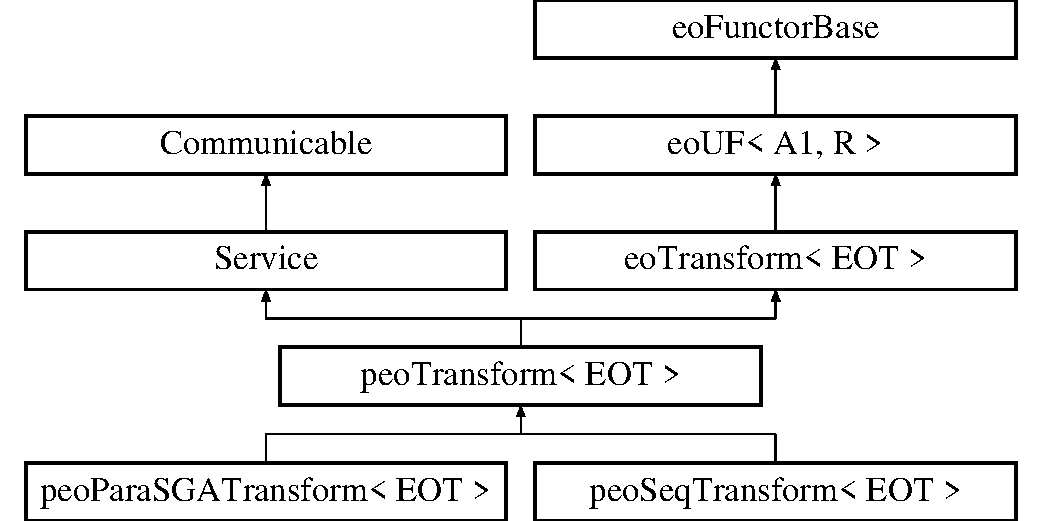
\includegraphics[height=4cm]{classpeoTransform}
\end{center}
\end{figure}


\subsection{Detailed Description}
\subsubsection*{template$<$class EOT$>$ class peo\-Transform$<$ EOT $>$}

The \hyperlink{classpeoTransform}{peo\-Transform} class acts only as an interface for creating transform operators - for an example please refer to the {\bf \hyperlink{classpeoSeqTransform}{peo\-Seq\-Transform}} and the {\bf \hyperlink{classpeoParaSGATransform}{peo\-Para\-SGATransform}} classes. 



Definition at line 20 of file peo\-Transform.h.

The documentation for this class was generated from the following file:\begin{CompactItemize}
\item 
peo\-Transform.h\end{CompactItemize}

\hypertarget{classReactiveThread}{
\section{Reactive\-Thread Class Reference}
\label{classReactiveThread}\index{ReactiveThread@{ReactiveThread}}
}
Inheritance diagram for Reactive\-Thread::\begin{figure}[H]
\begin{center}
\leavevmode
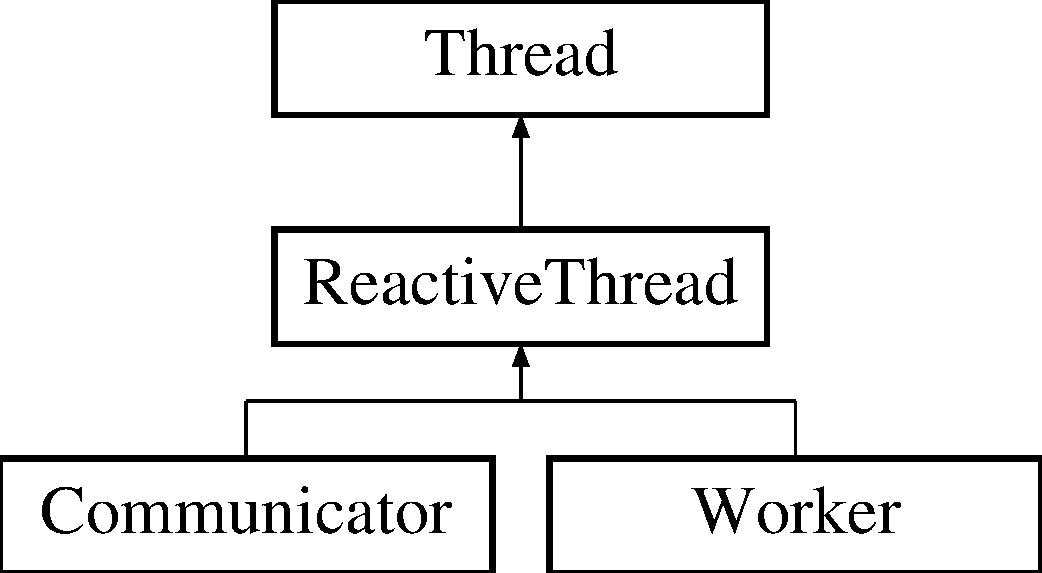
\includegraphics[height=3cm]{classReactiveThread}
\end{center}
\end{figure}
\subsection*{Public Member Functions}
\begin{CompactItemize}
\item 
\hypertarget{classReactiveThread_77381649429941c99a3e3d568113d6cf}{
\hyperlink{classReactiveThread_77381649429941c99a3e3d568113d6cf}{Reactive\-Thread} ()}
\label{classReactiveThread_77381649429941c99a3e3d568113d6cf}

\item 
\hypertarget{classReactiveThread_8263c2a32d8c99a49a05f1a7717d4262}{
void \hyperlink{classReactiveThread_8263c2a32d8c99a49a05f1a7717d4262}{sleep} ()}
\label{classReactiveThread_8263c2a32d8c99a49a05f1a7717d4262}

\item 
\hypertarget{classReactiveThread_a724a54575de10f09cc03ab7aa4e59ce}{
void \hyperlink{classReactiveThread_a724a54575de10f09cc03ab7aa4e59ce}{wake\-Up} ()}
\label{classReactiveThread_a724a54575de10f09cc03ab7aa4e59ce}

\end{CompactItemize}
\subsection*{Private Attributes}
\begin{CompactItemize}
\item 
\hypertarget{classReactiveThread_915e5a42dc8cb1bcf6738d5fe883a4e7}{
sem\_\-t \hyperlink{classReactiveThread_915e5a42dc8cb1bcf6738d5fe883a4e7}{sem}}
\label{classReactiveThread_915e5a42dc8cb1bcf6738d5fe883a4e7}

\end{CompactItemize}


\subsection{Detailed Description}




Definition at line 44 of file reac\_\-thread.h.

The documentation for this class was generated from the following files:\begin{CompactItemize}
\item 
reac\_\-thread.h\item 
reac\_\-thread.cpp\end{CompactItemize}

\hypertarget{classRingTopology}{
\section{Ring\-Topology Class Reference}
\label{classRingTopology}\index{RingTopology@{RingTopology}}
}
Inheritance diagram for Ring\-Topology::\begin{figure}[H]
\begin{center}
\leavevmode
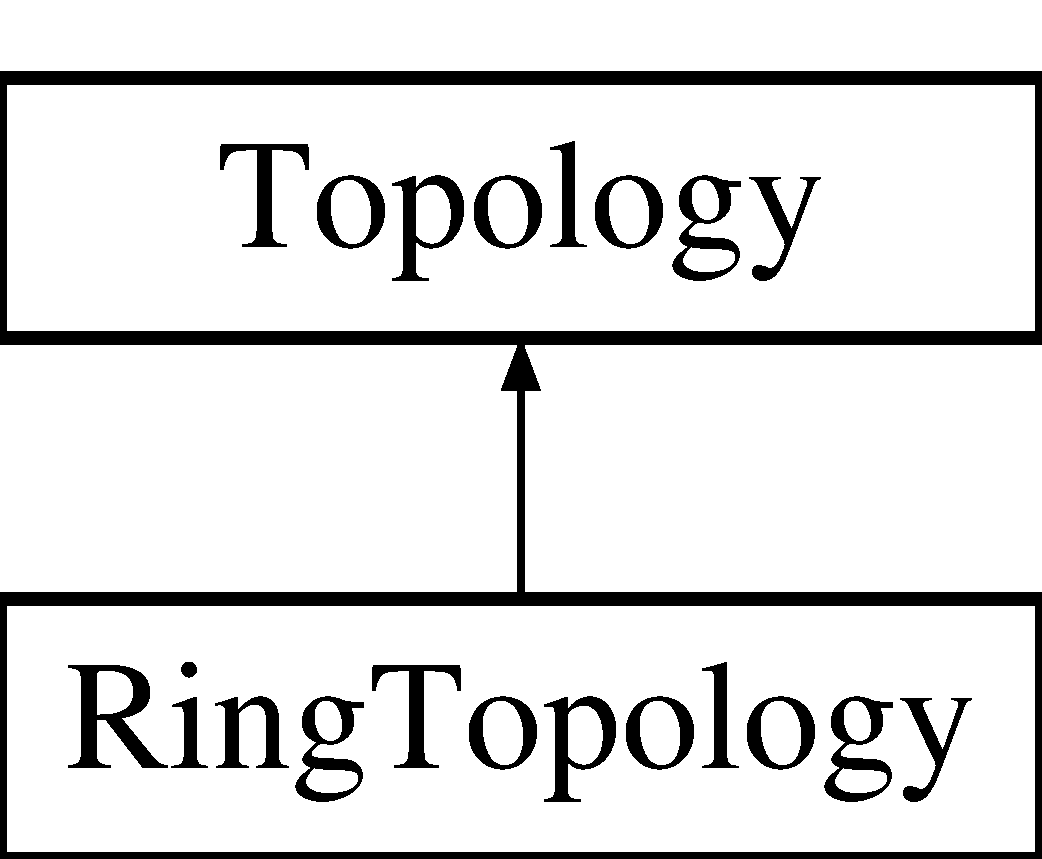
\includegraphics[height=2cm]{classRingTopology}
\end{center}
\end{figure}
\subsection*{Public Member Functions}
\begin{CompactItemize}
\item 
\hypertarget{classRingTopology_292a7746993788f96042f2f628cfcbc5}{
void \hyperlink{classRingTopology_292a7746993788f96042f2f628cfcbc5}{set\-Neighbors} (\hyperlink{classCooperative}{Cooperative} $\ast$\_\-\_\-mig, std::vector$<$ \hyperlink{classCooperative}{Cooperative} $\ast$ $>$ \&\_\-\_\-from, std::vector$<$ \hyperlink{classCooperative}{Cooperative} $\ast$ $>$ \&\_\-\_\-to)}
\label{classRingTopology_292a7746993788f96042f2f628cfcbc5}

\end{CompactItemize}


\subsection{Detailed Description}




Definition at line 42 of file ring\_\-topo.h.

The documentation for this class was generated from the following files:\begin{CompactItemize}
\item 
ring\_\-topo.h\item 
ring\_\-topo.cpp\end{CompactItemize}

\hypertarget{classRunner}{
\section{Runner Class Reference}
\label{classRunner}\index{Runner@{Runner}}
}
Inheritance diagram for Runner::\begin{figure}[H]
\begin{center}
\leavevmode
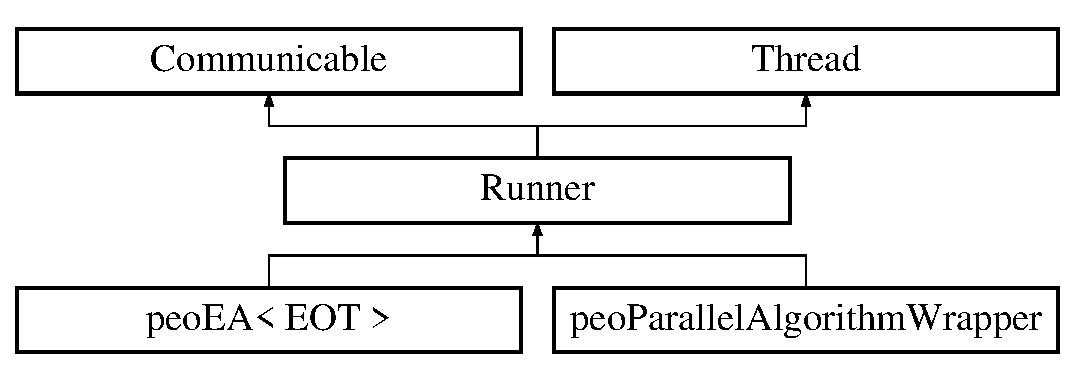
\includegraphics[height=3cm]{classRunner}
\end{center}
\end{figure}
\subsection*{Public Member Functions}
\begin{CompactItemize}
\item 
\hypertarget{classRunner_7acb8258c21da9daa62f9a177a2e5acd}{
\hyperlink{classRunner_7acb8258c21da9daa62f9a177a2e5acd}{Runner} ()}
\label{classRunner_7acb8258c21da9daa62f9a177a2e5acd}

\item 
\hypertarget{classRunner_7dc4419051fcc5cc9dadd54ecc9cd47d}{
void \hyperlink{classRunner_7dc4419051fcc5cc9dadd54ecc9cd47d}{start} ()}
\label{classRunner_7dc4419051fcc5cc9dadd54ecc9cd47d}

\item 
\hypertarget{classRunner_5bc239db2be753b77369fa9a038769fd}{
void \hyperlink{classRunner_5bc239db2be753b77369fa9a038769fd}{wait\-Starting} ()}
\label{classRunner_5bc239db2be753b77369fa9a038769fd}

\item 
\hypertarget{classRunner_40adbfb7d6944189b4fff60b02e669ca}{
bool \hyperlink{classRunner_40adbfb7d6944189b4fff60b02e669ca}{is\-Local} ()}
\label{classRunner_40adbfb7d6944189b4fff60b02e669ca}

\item 
\hypertarget{classRunner_0f133e75c28fb8264549814f80608e68}{
void \hyperlink{classRunner_0f133e75c28fb8264549814f80608e68}{terminate} ()}
\label{classRunner_0f133e75c28fb8264549814f80608e68}

\item 
\hypertarget{classRunner_5026c74eec184e3a15cb3c0ec4200a57}{
RUNNER\_\-ID \hyperlink{classRunner_5026c74eec184e3a15cb3c0ec4200a57}{get\-ID} ()}
\label{classRunner_5026c74eec184e3a15cb3c0ec4200a57}

\item 
\hypertarget{classRunner_2ad6d199d684d6f34347fc202ffe2fa3}{
void \hyperlink{classRunner_2ad6d199d684d6f34347fc202ffe2fa3}{pack\-Termination} ()}
\label{classRunner_2ad6d199d684d6f34347fc202ffe2fa3}

\item 
\hypertarget{classRunner_3591be473e0fcee1105fb57319b529aa}{
void \hyperlink{classRunner_3591be473e0fcee1105fb57319b529aa}{notify\-Sending\-Termination} ()}
\label{classRunner_3591be473e0fcee1105fb57319b529aa}

\end{CompactItemize}
\subsection*{Private Attributes}
\begin{CompactItemize}
\item 
\hypertarget{classRunner_4b0827d5df2df632db4ab71dd55e81b2}{
sem\_\-t \hyperlink{classRunner_4b0827d5df2df632db4ab71dd55e81b2}{sem\_\-start}}
\label{classRunner_4b0827d5df2df632db4ab71dd55e81b2}

\item 
\hypertarget{classRunner_1989c1f8e0b0b54ad2e60a341007e59d}{
unsigned \hyperlink{classRunner_1989c1f8e0b0b54ad2e60a341007e59d}{id}}
\label{classRunner_1989c1f8e0b0b54ad2e60a341007e59d}

\end{CompactItemize}


\subsection{Detailed Description}




Definition at line 47 of file runner.h.

The documentation for this class was generated from the following files:\begin{CompactItemize}
\item 
runner.h\item 
core/runner.cpp\item 
rmc/mpi/runner.cpp\end{CompactItemize}

\hypertarget{structSEND__REQUEST}{
\section{SEND\_\-REQUEST Struct Reference}
\label{structSEND__REQUEST}\index{SEND_REQUEST@{SEND\_\-REQUEST}}
}
\subsection*{Public Attributes}
\begin{CompactItemize}
\item 
\hypertarget{structSEND__REQUEST_1ad8f7233fa3ff13262e783a9153920f}{
\hyperlink{classCommunicable}{Communicable} $\ast$ \hyperlink{structSEND__REQUEST_1ad8f7233fa3ff13262e783a9153920f}{comm}}
\label{structSEND__REQUEST_1ad8f7233fa3ff13262e783a9153920f}

\item 
\hypertarget{structSEND__REQUEST_93e2a6a71d2a91aa2b7bdd050ee59b4d}{
int \hyperlink{structSEND__REQUEST_93e2a6a71d2a91aa2b7bdd050ee59b4d}{to}}
\label{structSEND__REQUEST_93e2a6a71d2a91aa2b7bdd050ee59b4d}

\item 
\hypertarget{structSEND__REQUEST_3126b3ef9d6533d3086760e413a7f23f}{
int \hyperlink{structSEND__REQUEST_3126b3ef9d6533d3086760e413a7f23f}{tag}}
\label{structSEND__REQUEST_3126b3ef9d6533d3086760e413a7f23f}

\end{CompactItemize}


\subsection{Detailed Description}




Definition at line 52 of file send.cpp.

The documentation for this struct was generated from the following file:\begin{CompactItemize}
\item 
send.cpp\end{CompactItemize}

\hypertarget{classService}{
\section{Service Class Reference}
\label{classService}\index{Service@{Service}}
}
Inheritance diagram for Service::\begin{figure}[H]
\begin{center}
\leavevmode
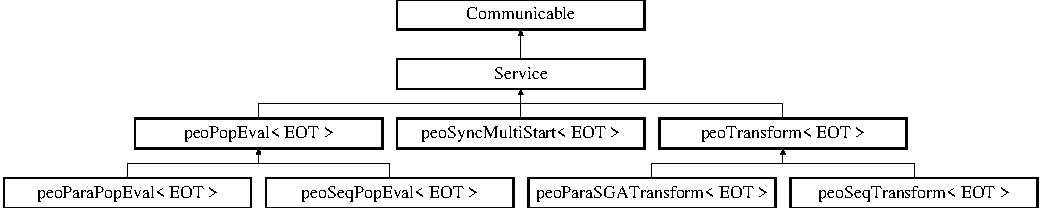
\includegraphics[height=2.8cm]{classService}
\end{center}
\end{figure}
\subsection*{Public Member Functions}
\begin{CompactItemize}
\item 
\hypertarget{classService_33b149b98498c0e7e401b0f0839d7f0d}{
void \hyperlink{classService_33b149b98498c0e7e401b0f0839d7f0d}{set\-Owner} (\hyperlink{classThread}{Thread} \&\_\-\_\-owner)}
\label{classService_33b149b98498c0e7e401b0f0839d7f0d}

\item 
\hypertarget{classService_0dae00309c51a7b7069788142aed799f}{
\hyperlink{classThread}{Thread} $\ast$ \hyperlink{classService_0dae00309c51a7b7069788142aed799f}{get\-Owner} ()}
\label{classService_0dae00309c51a7b7069788142aed799f}

\item 
\hypertarget{classService_7e2ae35a9070a05dcd46488df649896d}{
void \hyperlink{classService_7e2ae35a9070a05dcd46488df649896d}{request\-Resource\-Request} (unsigned \_\-\_\-how\_\-many=1)}
\label{classService_7e2ae35a9070a05dcd46488df649896d}

\item 
\hypertarget{classService_c4289f98d1cd9ed53e850efbb6a947bd}{
void \hyperlink{classService_c4289f98d1cd9ed53e850efbb6a947bd}{pack\-Resource\-Request} ()}
\label{classService_c4289f98d1cd9ed53e850efbb6a947bd}

\item 
\hypertarget{classService_aea4b8f7f8fb88e83862ee4bfd9ab207}{
virtual void \hyperlink{classService_aea4b8f7f8fb88e83862ee4bfd9ab207}{pack\-Data} ()}
\label{classService_aea4b8f7f8fb88e83862ee4bfd9ab207}

\item 
\hypertarget{classService_3bd87b444710813d30fd754d4d0b4df3}{
virtual void \hyperlink{classService_3bd87b444710813d30fd754d4d0b4df3}{unpack\-Data} ()}
\label{classService_3bd87b444710813d30fd754d4d0b4df3}

\item 
\hypertarget{classService_e4f2894e6121e60f38d41cfbd7447ae4}{
virtual void \hyperlink{classService_e4f2894e6121e60f38d41cfbd7447ae4}{execute} ()}
\label{classService_e4f2894e6121e60f38d41cfbd7447ae4}

\item 
\hypertarget{classService_e5e4f90b2315e15c2a2913bd370f4cf5}{
virtual void \hyperlink{classService_e5e4f90b2315e15c2a2913bd370f4cf5}{pack\-Result} ()}
\label{classService_e5e4f90b2315e15c2a2913bd370f4cf5}

\item 
\hypertarget{classService_45c06344edbfa482b91f68e2035a6099}{
virtual void \hyperlink{classService_45c06344edbfa482b91f68e2035a6099}{unpack\-Result} ()}
\label{classService_45c06344edbfa482b91f68e2035a6099}

\item 
\hypertarget{classService_81ad4d6ebb50045b8977e2ab74826f30}{
virtual void \hyperlink{classService_81ad4d6ebb50045b8977e2ab74826f30}{notify\-Sending\-Data} ()}
\label{classService_81ad4d6ebb50045b8977e2ab74826f30}

\item 
\hypertarget{classService_94e2012e76aaae3aa8199250f558d503}{
virtual void \hyperlink{classService_94e2012e76aaae3aa8199250f558d503}{notify\-Sending\-Resource\-Request} ()}
\label{classService_94e2012e76aaae3aa8199250f558d503}

\item 
\hypertarget{classService_f94cc8a5c2665d4574041737e61e9ffc}{
virtual void \hyperlink{classService_f94cc8a5c2665d4574041737e61e9ffc}{notify\-Sending\-All\-Resource\-Requests} ()}
\label{classService_f94cc8a5c2665d4574041737e61e9ffc}

\end{CompactItemize}
\subsection*{Private Attributes}
\begin{CompactItemize}
\item 
\hypertarget{classService_8b615c65c876f342fe8209eb7e36d7b2}{
\hyperlink{classThread}{Thread} $\ast$ \hyperlink{classService_8b615c65c876f342fe8209eb7e36d7b2}{owner}}
\label{classService_8b615c65c876f342fe8209eb7e36d7b2}

\item 
\hypertarget{classService_a5b2ad9520bb3710b54348b99acebd58}{
unsigned \hyperlink{classService_a5b2ad9520bb3710b54348b99acebd58}{num\_\-sent\_\-rr}}
\label{classService_a5b2ad9520bb3710b54348b99acebd58}

\end{CompactItemize}


\subsection{Detailed Description}




Definition at line 17 of file service.h.

The documentation for this class was generated from the following files:\begin{CompactItemize}
\item 
service.h\item 
core/service.cpp\item 
rmc/mpi/service.cpp\end{CompactItemize}

\hypertarget{classThread}{
\section{Thread Class Reference}
\label{classThread}\index{Thread@{Thread}}
}
Inheritance diagram for Thread::\begin{figure}[H]
\begin{center}
\leavevmode
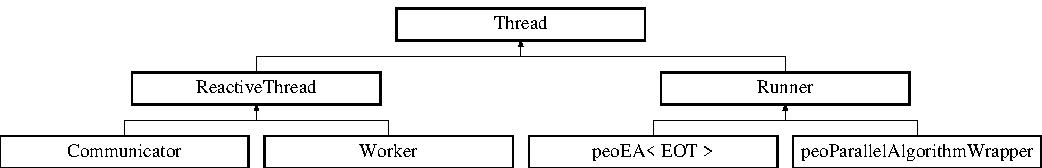
\includegraphics[height=3cm]{classThread}
\end{center}
\end{figure}
\subsection*{Public Member Functions}
\begin{CompactItemize}
\item 
\hypertarget{classThread_95c703fb8f2f27cb64f475a8c940864a}{
\hyperlink{classThread_95c703fb8f2f27cb64f475a8c940864a}{Thread} ()}
\label{classThread_95c703fb8f2f27cb64f475a8c940864a}

\item 
\hypertarget{classThread_37d9edd3a1a776cbc27dedff949c9726}{
virtual \hyperlink{classThread_37d9edd3a1a776cbc27dedff949c9726}{$\sim$Thread} ()}
\label{classThread_37d9edd3a1a776cbc27dedff949c9726}

\item 
\hypertarget{classThread_e197c46f8f62ecce6d2a7fe95bdc5b38}{
void \hyperlink{classThread_e197c46f8f62ecce6d2a7fe95bdc5b38}{set\-Active} ()}
\label{classThread_e197c46f8f62ecce6d2a7fe95bdc5b38}

\item 
\hypertarget{classThread_20632ffe9ddfa2a478afb0c84dc1096b}{
void \hyperlink{classThread_20632ffe9ddfa2a478afb0c84dc1096b}{set\-Passive} ()}
\label{classThread_20632ffe9ddfa2a478afb0c84dc1096b}

\end{CompactItemize}
\subsection*{Private Attributes}
\begin{CompactItemize}
\item 
\hypertarget{classThread_1b155d63bca3096ac4a1d039aea83c7c}{
bool \hyperlink{classThread_1b155d63bca3096ac4a1d039aea83c7c}{act}}
\label{classThread_1b155d63bca3096ac4a1d039aea83c7c}

\end{CompactItemize}


\subsection{Detailed Description}




Definition at line 31 of file thread.h.

The documentation for this class was generated from the following files:\begin{CompactItemize}
\item 
thread.h\item 
thread.cpp\end{CompactItemize}

\hypertarget{classTopology}{
\section{Topology Class Reference}
\label{classTopology}\index{Topology@{Topology}}
}
Inheritance diagram for Topology::\begin{figure}[H]
\begin{center}
\leavevmode
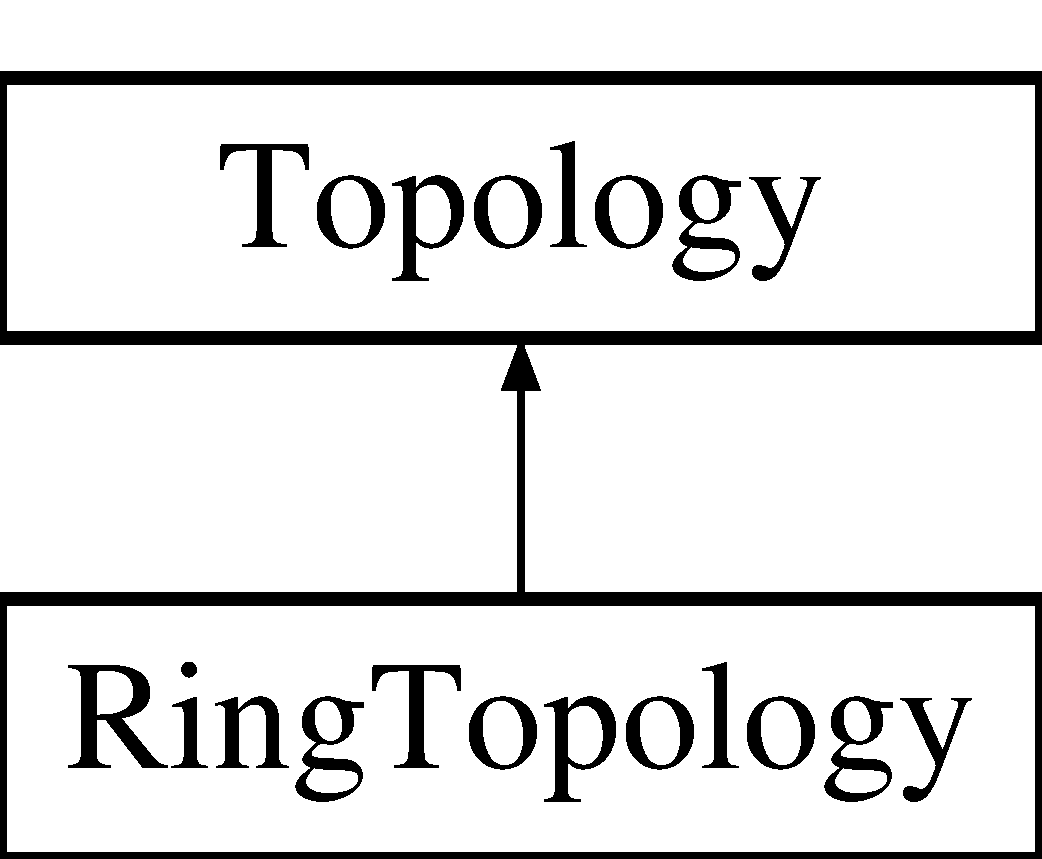
\includegraphics[height=2cm]{classTopology}
\end{center}
\end{figure}
\subsection*{Public Member Functions}
\begin{CompactItemize}
\item 
\hypertarget{classTopology_3e447669757c8311c7f6f8edc705abf2}{
virtual \hyperlink{classTopology_3e447669757c8311c7f6f8edc705abf2}{$\sim$Topology} ()}
\label{classTopology_3e447669757c8311c7f6f8edc705abf2}

\item 
\hypertarget{classTopology_62bc46d8c20fdc71dad9e7c7a0d7aded}{
void \hyperlink{classTopology_62bc46d8c20fdc71dad9e7c7a0d7aded}{add} (\hyperlink{classCooperative}{Cooperative} \&\_\-\_\-mig)}
\label{classTopology_62bc46d8c20fdc71dad9e7c7a0d7aded}

\end{CompactItemize}
\subsection*{Protected Attributes}
\begin{CompactItemize}
\item 
\hypertarget{classTopology_247a2faa8568b678f0b7b11e62c7812c}{
std::vector$<$ \hyperlink{classCooperative}{Cooperative} $\ast$ $>$ \hyperlink{classTopology_247a2faa8568b678f0b7b11e62c7812c}{mig}}
\label{classTopology_247a2faa8568b678f0b7b11e62c7812c}

\end{CompactItemize}


\subsection{Detailed Description}




Definition at line 16 of file topology.h.

The documentation for this class was generated from the following files:\begin{CompactItemize}
\item 
topology.h\item 
topology.cpp\end{CompactItemize}

\hypertarget{classWorker}{
\section{Worker Class Reference}
\label{classWorker}\index{Worker@{Worker}}
}
Inheritance diagram for Worker::\begin{figure}[H]
\begin{center}
\leavevmode
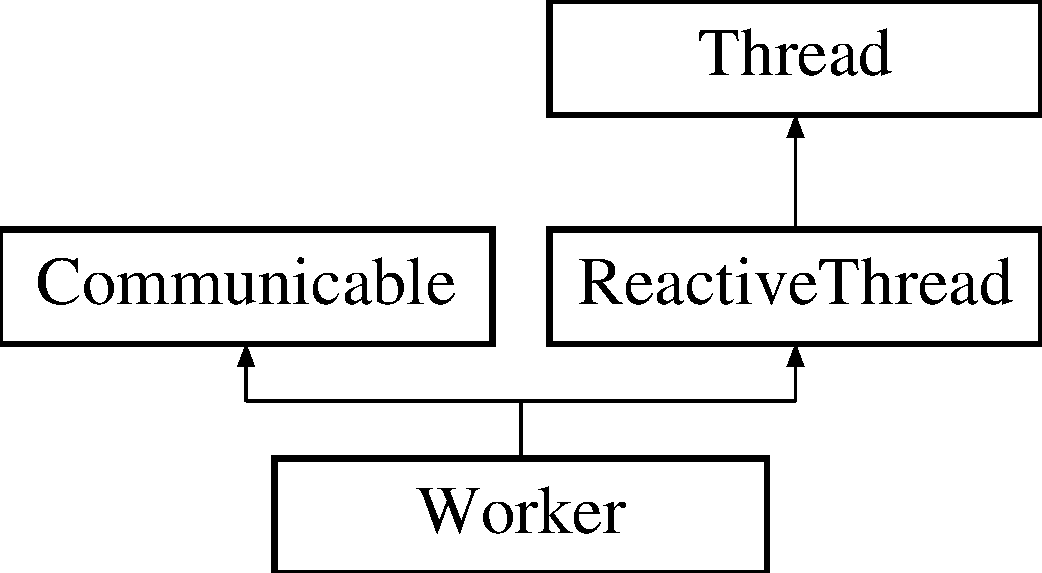
\includegraphics[height=3cm]{classWorker}
\end{center}
\end{figure}
\subsection*{Public Member Functions}
\begin{CompactItemize}
\item 
\hypertarget{classWorker_3754817df06ffe220f7f0d903c78ccac}{
\hyperlink{classWorker_3754817df06ffe220f7f0d903c78ccac}{Worker} ()}
\label{classWorker_3754817df06ffe220f7f0d903c78ccac}

\item 
\hypertarget{classWorker_abcbbace05c6113f1959c494b3577291}{
void \hyperlink{classWorker_abcbbace05c6113f1959c494b3577291}{start} ()}
\label{classWorker_abcbbace05c6113f1959c494b3577291}

\item 
\hypertarget{classWorker_83780920118e6c2b67d9477bdf8be248}{
void \hyperlink{classWorker_83780920118e6c2b67d9477bdf8be248}{pack\-Result} ()}
\label{classWorker_83780920118e6c2b67d9477bdf8be248}

\item 
\hypertarget{classWorker_bff2bdcd64fe5400156cc78704c64953}{
void \hyperlink{classWorker_bff2bdcd64fe5400156cc78704c64953}{unpack\-Data} ()}
\label{classWorker_bff2bdcd64fe5400156cc78704c64953}

\item 
\hypertarget{classWorker_60d2e8eba85b9ef403d94be54c391640}{
void \hyperlink{classWorker_60d2e8eba85b9ef403d94be54c391640}{pack\-Task\-Done} ()}
\label{classWorker_60d2e8eba85b9ef403d94be54c391640}

\item 
\hypertarget{classWorker_e2f487014766a73c5788bdcfd58ad863}{
void \hyperlink{classWorker_e2f487014766a73c5788bdcfd58ad863}{notify\-Sending\-Result} ()}
\label{classWorker_e2f487014766a73c5788bdcfd58ad863}

\item 
\hypertarget{classWorker_13efd6a8e275745329a4a8e23a0eb0bb}{
void \hyperlink{classWorker_13efd6a8e275745329a4a8e23a0eb0bb}{notify\-Sending\-Task\-Done} ()}
\label{classWorker_13efd6a8e275745329a4a8e23a0eb0bb}

\item 
\hypertarget{classWorker_5dab4ea663546b5a49d9398d7a624d27}{
void \hyperlink{classWorker_5dab4ea663546b5a49d9398d7a624d27}{set\-Source} (int \_\-\_\-rank)}
\label{classWorker_5dab4ea663546b5a49d9398d7a624d27}

\end{CompactItemize}
\subsection*{Private Attributes}
\begin{CompactItemize}
\item 
\hypertarget{classWorker_b5ffcb995e12fa71b9551e91729d6972}{
WORKER\_\-ID \hyperlink{classWorker_b5ffcb995e12fa71b9551e91729d6972}{id}}
\label{classWorker_b5ffcb995e12fa71b9551e91729d6972}

\item 
\hypertarget{classWorker_d7dc76e301fd2bcf5d3a2088a59f1378}{
SERVICE\_\-ID \hyperlink{classWorker_d7dc76e301fd2bcf5d3a2088a59f1378}{serv\_\-id}}
\label{classWorker_d7dc76e301fd2bcf5d3a2088a59f1378}

\item 
\hypertarget{classWorker_454e1764ed165af733cc44a73e395692}{
\hyperlink{classService}{Service} $\ast$ \hyperlink{classWorker_454e1764ed165af733cc44a73e395692}{serv}}
\label{classWorker_454e1764ed165af733cc44a73e395692}

\item 
\hypertarget{classWorker_895c3ebc198018ea3391c09bc802d2f6}{
int \hyperlink{classWorker_895c3ebc198018ea3391c09bc802d2f6}{src}}
\label{classWorker_895c3ebc198018ea3391c09bc802d2f6}

\item 
\hypertarget{classWorker_7ba5a18b2918cf9e704536b763be37f7}{
bool \hyperlink{classWorker_7ba5a18b2918cf9e704536b763be37f7}{toto}}
\label{classWorker_7ba5a18b2918cf9e704536b763be37f7}

\end{CompactItemize}


\subsection{Detailed Description}




Definition at line 33 of file worker.h.

The documentation for this class was generated from the following files:\begin{CompactItemize}
\item 
worker.h\item 
worker.cpp\end{CompactItemize}

\printindex
\end{document}
